\documentclass[a4paper,10pt,oneside,openany,fleqno]{article}
%%%%%%%%%%%%%%%%%%%%%%%%%%%%%%%%%%%%%%%%%%%%%%%%%%%%%%%%%%%%
\usepackage{pgf-PeriodicTable}
\usepgfPTlibrary{colorschemes}%
%%%%%%%%%%%%%%%%%%%%%%%%%%%%%%%%%%%%%%%%%%%%%%%%%%%%%%%%%%%%
% Definitions for pgf-PeriodicTable Manual
% Hugo Gomes @ 10/02/2025 v2.1.5
% Hugo Gomes @ 08/09/2024 v2.1.4
% Hugo Gomes @ 07/08/2024 v2.1.3
% Hugo Gomes @ 01/08/2024 v2.1.2
% Hugo Gomes @ 07/07/2024 v2.1.1
% Hugo Gomes @ 03/04/2024 v2.1.0a
% Hugo Gomes @ 14/02/2024 v2.1.0
% Hugo Gomes @ 29/05/2023 v2.0.1
% Hugo Gomes @ 20/02/2023 v2.0.0
% Hugo Gomes @ 08/11/2022 v1.0.1
% Hugo Gomes @ 10/10/2022 v1.0.0
\def\pgfPTversion{2.1.5}%
\def\pgfPTnewinversion#1{new in v#1}%
\def\pgfPTchangedinversion#1{changed in v#1}%
%%%%%%%%%%%%%%%%%%%%%%%%%%%%%%%%%%%%%%%%%%%%%%%%%%%%%%%%%%%%
\usepackage[ansinew]{inputenc}
\usepackage{verdana}
%
\addtolength{\textwidth}{3.5cm}
\addtolength{\textheight}{2.5cm}
\addtolength{\topmargin}{-1.25cm}
\setlength{\parindent}{0pt}
\setlength{\oddsidemargin}{0pt}
\setcounter{secnumdepth}{1}%
\setcounter{tocdepth}{4}
%
%%%%%%%%%%%%%%%%%%%%%%%%%%%%%%%%%%%%%%%%%%%%%%%%%%%%%%%%%%%%
\pgfdeclarelayer{back}%
\pgfsetlayers{back,main}%
%%%%%%%%%%%%%%%%%%%%%%%%%%%%%%%%%%%%%%%%%%%%%%%%%%%%%%%%%%%%
\usetikzlibrary{shadows}%
%%%%%%%%%%%%%%%%%%%%%%%%%%%%%%%%%%%%%%%%%%%%%%%%%%%%%%%%%%%%
\usepackage{makeidx}
\makeindex%
% ------------------------------------------------------------------------------------------------------------------------------------
% BUILD SEQUENCE:
% 1) pdflatex.exe "pgf-PeriodicTableManual.tex"
% 2) makeindex.exe -s "pgf-PeriodicTableManual.ist" "pgf-PeriodicTableManual.idx"
% 3) pdflatex.exe "pgf-PeriodicTableManual.tex"
% ------------------------------------------------------------------------------------------------------------------------------------
\usepackage[skins]{tcolorbox}
\tcbuselibrary{breakable}
\usepackage[english]{babel}
\usepackage{pifont}
\usepackage[pdfstartview={ },colorlinks=true, linkcolor=black!50!green, citecolor=gray, urlcolor=teal, hyperindex, plainpages=false,bookmarksopenlevel=1,bookmarksopen=true]{hyperref}%
\hypersetup{%Start options on pdf
pdftitle = {Manual for pgf-PeriodicTable (v\pgfPTversion)},%
pdfsubject = {Periodic Table of Elements},%
pdfkeywords = {Draw the Periodic Table of Elements in a simple way via pgf/TikZ environment. It's possible to draw a full or partial Periodic Table of Elements},%
pdfauthor = {\textcopyright Hugo Gomes},%
pdfproducer = {pdfeTeX-1.\the\pdftexversion\pdftexrevision},
}%End options on pdf
\usepackage{fancyhdr}
\usepackage{lastpage}
\renewcommand{\headrulewidth}{0.4pt}%
\renewcommand{\footrulewidth}{0.4pt}%
\addtolength{\headheight}{25pt}%
\fancypagestyle{pgfPTManual}{%
\fancyhf{} % clear all header and footer fields
\fancyhead[R]{\usefont{T1}{vna}{m}{n}\nouppercase{\leftmark}}%
\fancyhead[L]{\color{blue!70!black}pgf-PeriodicTable \pgfPTversion}%
\fancyfoot[R]{\usefont{T1}{vna}{m}{n}\textbf{\thepage\ of \pageref{LastPage}}}%
\fancyfoot[L]{\ }}%
\fancypagestyle{plain}{%
\addtolength{\textwidth}{3.5cm}%
\fancyhf{} % clear all header and footer fields
\fancyhead[R]{\usefont{T1}{vna}{m}{n}\nouppercase{\leftmark}}%
\fancyhead[L]{\color{blue!70!black}pgf-PeriodicTable \pgfPTversion}%
\fancyfoot[R]{\usefont{T1}{vna}{m}{n}\textbf{\thepage\ of \pageref{LastPage}}}%
\fancyfoot[L]{\ }}%
\usepackage{amsfonts}
\usepackage{amssymb}
\usepackage{amsmath}
\usepackage{tabularx}
\usepackage{calc}
%%%%%%%%%%%%%%%%%%%%%%%%%%%%%%%%%%%%%%%%%%%%%%%%%%%%%%%%%%%%
\makeatletter%
\renewenvironment{theindex}%
               {\if@twocolumn%
                  \@restonecolfalse%
                \else%
                  \@restonecoltrue%
                \fi%
%             \twocolumn[\section*{\indexname}]%
                \twocolumn[\section{\indexname}]%
                \@mkboth{\MakeUppercase\indexname}%
                        {\MakeUppercase\indexname}%
                \thispagestyle{plain}\parindent\z@%
                \parskip\z@ \@plus .3\p@\relax%
                \columnseprule \z@%
                \columnsep 35\p@%
                \let\item\@idxitem}%
               {\if@restonecol\onecolumn\else\clearpage\fi}%
%%%%%%%%%%%%%%%%%%%%%%%%%%%%%%%%%%%%%%%%%%%%%%%%%%%%%%%%%%%%
\def\pack{\large\texttt{\color{blue!70!black}pgf-PeriodicTable}\normalsize}%
\def\txttt#1{\large\texttt{#1}\normalsize}%
\def\txttikz{{\fontfamily{cmr}\selectfont Ti\emph{k}Z}}%
\def\ie{\textit{i.e.\/}}%
\def\eg{\textit{e.g.\/}}%
\def\myldots{\tikz{\fill (0,0) circle(.6pt);\fill (2.4pt,0) circle(.6pt);\fill (4.8pt,0) circle(.6pt);}}%
\def\cyan#1{\textcolor{cyan!50!black}{#1}}%
\def\dcyan#1{\textcolor{cyan!30!black}{#1}}%
\def\gray#1{\textcolor{black!50}{#1}}%
\def\blue#1{\textcolor{blue!50!black}{#1}}%
\def\lblue#1{\textcolor{blue!70!black}{#1}}%
\def\green#1{\textcolor{green!50!black}{#1}}%
\def\red#1{\textcolor{red!50!black}{#1}}%
\def\orange#1{\textcolor{orange!80!black}{#1}}%
\def\bs#1{\textcolor{blue!50!black}{\textbackslash#1}}%
\def\lb{\textcolor{blue!50!black}{\{}}%
\def\rb{\textcolor{blue!50!black}{\}}}%
\def\lp{\textcolor{blue!50!black}{[}}%
\def\rp{\textcolor{blue!50!black}{]}}%
\def\fnt#1#2{\begingroup\fontfamily{#1}\selectfont#1\ -- #2\endgroup}%
\def\pgfPTM@quote{\tikz{\pgfmathparse{height("l")}\edef\@lht{\pgfmathresult}\draw[line width=.75pt,line cap=round] (0,0) (0,\@lht-.65pt) -- ++(0,-1.65pt);}}
\def\sq#1{\pgfPTM@quote\makebox[.875pt][s]{}\textcolor{green!50!black}{#1}\makebox[.875pt][s]{}\pgfPTM@quote}%
%%%%%%%%%%%%%%%%%%%%%%%%%%%%%%%%%%%%%%%%%%%%%%%%%%%%%%%%%%%%
\def\pgfPTMcolorDemo#1#2{\setbox0=\hbox{\makebox[23pt][s]{}#2}\vbox to 8pt{\hsize=\wd0\tikz{\draw[#1!50!black,fill=#1,rounded corners=2pt] (0,0) rectangle (20pt,8pt);\node[font=\small,right,inner sep=0pt] at (23pt,2.75pt) {#2};}}}%
\def\pgfPTMselectfont{\string\selectfont}%
\def\pgfPTMtiny{\string\tiny}%
\def\pgfPTMscriptsize{\string\scriptsize}%
\def\pgfPTMfootnotesize{\string\footnotesize}%
\def\pgfPTMsmall{\string\small}%
\def\pgfPTMlarge{\string\large}%
\def\pgfPTMLarge{\string\Large}%
\def\pgfPTMLARGE{\string\LARGE}%
\def\pgfPTMhuge{\string\huge}%
\def\pgfPTMHuge{\string\Huge}%
\def\pgfPTMitshape{\string\itshape}%
\def\pgfPTMbfseries{\string\bfseries}%
%%%%%%%%%%%%%%%%%%%%%%%%%%%%%%%%%%%%%%%%%%%%%%%%%%%%%%%%%%%%
\def\pgfPTMzerodepth#1{{\setbox0=\hbox{#1}\dp0=0pt\box0\relax}}%
\def\pgfPTMparbox#1{{\setbox0=\vbox{\parshape=2 0pt \linewidth 10pt \the\dimexpr \linewidth-10pt\relax{#1}}\usebox0\relax}}%
\def\pgfPTMline{\tikz{\fill[black!10,rounded corners=2pt] (0,0) rectangle (\linewidth,-4pt);}}%
%%%%%%%%%%%%%%%%%%%%%%%%%%%%%%%%%%%%%%%%%%%%%%%%%%%%%%%%%%%%
\newdimen\pgfPTMspace\pgfPTMspace=0pt%
% \pgfPTmacro{macro name}[options list]
\def\pgfPTMmacro#1[#2]{\ignorespaces%
\edef\pgfPTM@optionslist{#2}%
\ifx\pgfPTM@optionslist\@empty\relax\textcolor{blue!50!black}{\textbackslash #1}%
\else%
\textcolor{blue!50!black}{\textbackslash #1[}\textcolor{red!50!black}{\detokenize\expandafter{\pgfPTM@optionslist}}\textcolor{blue!50!black}{]}%
\fi%
}%
%%%%%%%%%%%%%%%%%%%%%%%%%%%%%%%%%%%%%%%%%%%%%%%%%%%%%%%%%%%%
% \pgfPTmacrobox[alignment]{macro name}[options list]
\def\pgfPTMmacrobox{\@ifnextchar[\pgfPTM@macrobox{\pgfPTM@macrobox[c]}}%
\def\pgfPTM@macrobox[#1]#2[#3]{\ignorespaces%
\edef\pgfPTM@optionslist{#3}%
\edef\pgfPTM@align{#1}\edef\pgfPTM@align@c{c}%
\ifx\pgfPTM@align\pgfPTM@align@c\relax\def\pgfPTM@alignment{flush center}\else\def\pgfPTM@alignment{left}\fi%
\ifx\pgfPTM@optionslist\@empty\relax%
\tikz{\node[text width=\linewidth-8pt,inner xsep=4pt,align=\pgfPTM@alignment,fill=black!10,rounded corners=2pt] %
{\textcolor{blue!50!black}{\textbackslash #2}};}%
\else%
\tikz{\node[text width=\linewidth-8pt,inner xsep=4pt,align=\pgfPTM@alignment,fill=black!10,rounded corners=2pt] %
{\textcolor{blue!50!black}{\textbackslash #2[}\textcolor{red!50!black}{\detokenize\expandafter{\pgfPTM@optionslist}}\textcolor{blue!50!black}{]}};}%
\fi%
}%
%%%%%%%%%%%%%%%%%%%%%%%%%%%%%%%%%%%%%%%%%%%%%%%%%%%%%%%%%%%%
\definecolor{cItemList}{rgb}{0.55,0.78,0.25}
\newenvironment{itemlist}{%
\begin{list}{\hfill$\boldsymbol{\checkmark}$}{\setlength{\parsep}{0pt}\setlength{\topsep}{4pt}\setlength{\leftmargin}{6mm}\setlength{\labelwidth}{1em}\setlength{\labelsep}{1pt}}}{\end{list}}
\tcolorboxenvironment{itemlist}{breakable,blanker,before skip=2pt,after skip=4pt,
                                                borderline west={2.8pt}{.75pt}{cItemList!75!black},
                                                borderline west={2.8pt}{3.55pt}{cItemList!75!black!50!white},
                                                borderline west={2.8pt}{6.35pt}{cItemList!25!white}}%
\newenvironment{itembar}{\footnotesize%
\begin{list}{\hfill$\boldsymbol{\checkmark}$}{\setlength{\parsep}{0pt}\setlength{\topsep}{4pt}\setlength{\leftmargin}{6mm}\setlength{\labelwidth}{1em}\setlength{\labelsep}{1pt}}}{\end{list}}
\tcolorboxenvironment{itembar}{breakable,blanker,before skip=6pt,after skip=6pt,
                                                borderline west={2.8pt}{.75pt}{blue!75!black},
                                                borderline west={2.8pt}{3.55pt}{blue!75!black!50!white},
                                                borderline west={2.8pt}{6.35pt}{blue!25!white}}%
\newtcbox{\use}{enhanced,nobeforeafter,tcbox raise base,boxrule=0.4pt,top=0mm,bottom=0mm,%
  right=0mm,left=15mm,arc=1pt,boxsep=2pt,%
  colframe=cyan!50!black,coltext=cyan!25!black,colback=cyan!10!white,fontupper=\scriptsize,%
  overlay={\begin{tcbclipinterior}\fill[cyan!50!white] (frame.south west)%
    rectangle node[text=white,font=\scriptsize\bfseries,anchor=mid] {USAGE:} ([xshift=15mm]frame.north west);\end{tcbclipinterior}}}
\newtcbox{\uselib}{enhanced,nobeforeafter,tcbox raise base,boxrule=0.4pt,top=0mm,bottom=0mm,%
  right=0mm,left=15mm,arc=1pt,boxsep=2pt,%
  colframe=cyan!50!black,coltext=cyan!25!black,colback=cyan!10!white,fontupper=\small,%
  overlay={\begin{tcbclipinterior}\fill[cyan!50!white] (frame.south west)%
    rectangle node[text=white,font=\small\bfseries,anchor=mid] {USAGE: } ([xshift=15mm]frame.north west);\end{tcbclipinterior}}}%
\newcommand\mymfbox[2][gray]{\begin{tcolorbox}
[breakable,enhanced,arc=2.5pt,outer arc=2.5pt,colback=#1!10!white,colframe=#1!50!black,boxsep=3pt,left=3pt,right=3pt,top=3pt,bottom=3pt,boxrule=1pt]
#2\end{tcolorbox}}
\def\mysmile{\tikz[scale=1.2]{\path[fill=yellow] (0,0) circle (.15cm);
                               \fill[black!90] (45:.9mm) circle (.175mm);
                               \fill[black!90] (135:.9mm) circle (.175mm);
                               \draw[line width=.15mm,black!90] (215:.9mm) arc (215:325:.9mm);}}
\newcommand\tcexemplo[2][EXEMPLO:]{\begin{tcolorbox}[breakable,enhanced,fonttitle=\bfseries,
                            colback=green!5!white,colframe=white!50!green,title=#1,after title={\hfill\mysmile},
                            ]
                            #2
                            \end{tcolorbox}}
%%%%%%%%%%%%%%%%%%%%%%%%%%%%%%%%%%%%%%%%%%%%%%%%%%%%%%%%%%%%
% \pgfPTMbuildcell(lines,columns)[entries]
\def\pgfPTMbuildcell(#1,#2)[#3]{\ignorespaces%
\tikz{\node[text width=\linewidth-8pt,inner xsep=4pt,align=left,fill=black!10,rounded corners=2pt] %
{\textcolor{blue!50!black}{\textbackslash pgfPTbuildcell(}\textcolor{red!50!black}{#1,#2}\textcolor{blue!50!black}{)}%
\textcolor{black!50}{\% #1\ rows by #2 columns}\\ \textcolor{blue!50!black}{[}%
\textcolor{red!50!black}{\detokenize\expandafter{#3}}\textcolor{blue!50!black}{]}};}%
}%
%%%%%%%%%%%%%%%%%%%%%%%%%%%%%%%%%%%%%%%%%%%%%%%%%%%%%%%%%%%%
% \pgfPTMbtn{txt}
\definecolor{btnBack}{RGB}{237,237,237}%
\definecolor{btnBorder}{RGB}{127,116,112}%
\def\pgfPTMbtn#1{\tikz[baseline=(X.base)]{\node[draw=btnBorder,fill=btnBack,rounded corners=1.5pt,inner sep=2pt,font=\small,text=black,anchor=base] (X) {\pgfPT@box@zerodepth{#1}};}}%
%%%%%%%%%%%%%%%%%%%%%%%%%%%%%%%%%%%%%%%%%%%%%%%%%%%%%%%%%%%%
% \pgfPTMbuildcellstyle{name}(lines,columns)[entries]
\def\pgfPTMbuildcellstyle#1(#2,#3)[#4]{\ignorespaces%
\tikz{\node[text width=\linewidth-8pt,inner xsep=4pt,align=left,fill=black!10,rounded corners=2pt] %
{\textcolor{blue!50!black}{\textbackslash pgfPTbuildcellstyle\{}\textcolor{red!50!black}{#1}\textcolor{blue!50!black}{\}}%
\textcolor{blue!50!black}{(}\textcolor{red!50!black}{#2,#3}\textcolor{blue!50!black}{)}%
\textcolor{black!50}{\% #2\ rows by #3 columns}\\ \textcolor{blue!50!black}{[}%
\textcolor{red!50!black}{\detokenize\expandafter{#4}}\textcolor{blue!50!black}{]}};}%
}%
%%%%%%%%%%%%%%%%%%%%%%%%%%%%%%%%%%%%%%%%%%%%%%%%%%%%%%%%%%%%
% \pgfPTMpreviewcellstyle[scale factor]{name}
\def\pgfPTMpreviewcellstyle[#1]#2{\ignorespaces%
\edef\pgfPTM@optionslist{#1}%
\ifx\pgfPTM@optionslist\@empty\relax%
\tikz{\node[text width=\linewidth-8pt,inner xsep=4pt,align=center,fill=black!10,rounded corners=2pt] %
{\textcolor{blue!50!black}{\textbackslash pgfPTpreviewcellstyle\{}\textcolor{red!50!black}{#2}\textcolor{blue!50!black}{\}}};}%
\else%
\tikz{\node[text width=\linewidth-8pt,inner xsep=4pt,align=center,fill=black!10,rounded corners=2pt] %
{\textcolor{blue!50!black}{\textbackslash pgfPTpreviewcellstyle[}\textcolor{red!50!black}{#1}\textcolor{blue!50!black}{]\{}%
\textcolor{red!50!black}{#2}\textcolor{blue!50!black}{\}}};}%
\fi%
}%
%%%%%%%%%%%%%%%%%%%%%%%%%%%%%%%%%%%%%%%%%%%%%%%%%%%%%%%%%%%%
% \pgfPTMpreviewcellstyle(line;column;what)(line_i to line_f)(column_i to column_f)
\def\pgfPTMcelldesign(#1;#2;#3)(#4 to #5)(#6 to #7){%
\makebox[\linewidth][c]{\begin{tikzpicture}
\draw[line width=1pt,fill=black!10] (0,0) rectangle ++(3,-4);
\foreach \x in {1,2}{\draw[dotted,line width=.8pt,red] (\x cm,0) node[above,xshift=-.5cm] {\x} -- ++(0,-4);}\node[red,above] at (2.5,0) {3};
\foreach \y in {1,...,4}{\draw[dotted,line width=.8pt,blue] (0,-.8*\y cm) node[left,yshift=.4cm] {\y} -- ++(3,0);}\node[blue,left] at (0,-3.6) {5};
\draw[line width=1pt,double distance=1pt,-stealth] (3.5,-2) -- ++(3,0) node[midway,above] {\green{(#1;#2;#3)}};
\draw[line width=1pt,fill=black!10] (7,0) rectangle ++(3,-4);
\foreach \x in {1,2}{\draw[dotted,line width=.8pt,red] (7cm+\x cm,0) node[above,xshift=-.5cm] {\x} -- ++(0,-4);}\node[red,above] at (9.5,0) {3};
\foreach \y in {1,...,4}{\draw[dotted,line width=.8pt,blue] (7cm,-.8*\y cm) node[left,yshift=.4cm] {\y} -- ++(3,0);}\node[blue,left] at (7,-3.6) {5};
\draw[green!50!black,fill=green!50!white,opacity=.5] (6cm+#6cm,-0.8*#4cm+.8cm) rectangle ++(#7cm-#6cm,-.8*#5cm+.8*#4cm) node[midway,opacity=1] {\green{#3}};
\end{tikzpicture}}}
%%%%%%%%%%%%%%%%%%%%%%%%%%%%%%%%%%%%%%%%%%%%%%%%%%%%%%%%%%%%
% \pgfPTMnewColorScheme[<trailing color (default=1/1/1 e.g. white)>]{name}{list}
\def\pgfPTMnewColorScheme[#1]#2#3{\ignorespaces%
\edef\pgfPTM@optionslist{#1}%
\ifx\pgfPTM@optionslist\@empty\relax%
\tikz{\node[text width=\linewidth-8pt,inner xsep=4pt,align=center,fill=black!10,rounded corners=2pt] %
{\textcolor{blue!50!black}{\textbackslash pgfPTnewColorScheme\{}\textcolor{red!50!black}{#2}\textcolor{blue!50!black}{\}\{}%
\textcolor{red!50!black}{#3}\textcolor{blue!50!black}{\}}};}%
\else%
\tikz{\node[text width=\linewidth-8pt,inner xsep=4pt,align=center,fill=black!10,rounded corners=2pt] %
{\textcolor{blue!50!black}{\textbackslash pgfPTnewColorScheme[}\textcolor{red!50!black}{#1}\textcolor{blue!50!black}{]\{}%
\textcolor{red!50!black}{#2}\textcolor{blue!50!black}{\}\{}%
\textcolor{red!50!black}{#3}\textcolor{blue!50!black}{\}}};}%
\fi%
}%
%%%%%%%%%%%%%%%%%%%%%%%%%%%%%%%%%%%%%%%%%%%%%%%%%%%%%%%%%%%%
% \pgfPTMnewZlist{name}{list}
\def\pgfPTMnewZlist#1#2{\ignorespaces%
\tikz{\node[text width=\linewidth-8pt,inner xsep=4pt,align=center,fill=black!10,rounded corners=2pt] %
{\textcolor{blue!50!black}{\textbackslash pgfPTnewZlist\{}\textcolor{red!50!black}{#1}\textcolor{blue!50!black}{\}\{}%
\textcolor{red!50!black}{#2}\textcolor{blue!50!black}{\}}};}%
}%
%%%%%%%%%%%%%%%%%%%%%%%%%%%%%%%%%%%%%%%%%%%%%%%%%%%%%%%%%%%%
% \pgfPTMsetLanguage{language flag}
\def\pgfPTMsetLanguage#1{\ignorespaces%
\tikz{\node[text width=\linewidth-8pt,inner xsep=4pt,align=center,fill=black!10,rounded corners=2pt] %
{\textcolor{blue!50!black}{\textbackslash pgfPTsetLanguage\{}\textcolor{red!50!black}{#1}\textcolor{blue!50!black}{\}}};}%
}%
%%%%%%%%%%%%%%%%%%%%%%%%%%%%%%%%%%%%%%%%%%%%%%%%%%%%%%%%%%%%%
% \pgfPTMoption[version]{level}{option}{default}{description} level=3-> subsubsection; level=4-> paragraph
\def\pgfPTMoption{\@ifnextchar[\pgfPTM@option{\pgfPTM@option[]}}%
\def\pgfPTM@option[#1]#2#3#4#5{\index{OPTIONS@\textbf{OPTIONS}!#3}\ignorespaces%
\ifnum#2=3\relax\vskip-4.75ex\vskip-18pt\ \subsubsection*{}\addcontentsline{toc}{subsubsection}{\texorpdfstring{$\rightsquigarrow$ #3}{#3}}%
\else\ifnum#2=4\relax\vskip-4.75ex\vskip-20pt\ \paragraph*{}\addcontentsline{toc}{paragraph}{\texorpdfstring{$\rightsquigarrow$ #3}{#3}}\ \\ [8pt]%
\fi\fi%
\edef\pgfPTM@version{#1}%
\begin{tikzpicture}%
\node[below right,font=\small\bfseries] (a) at (0,0) {\hypertarget{option:#3}{#3}};%
\node[below left,font=\small] (b) at (\textwidth-.3333em,0) {default: \itshape#4};%
\node[below right,text=black!80,font=\small,text width=\textwidth-.6666em] (c) at (a.south west) %
{#5\ifx\pgfPTM@version\@empty\relax\else\hfill\textit{\textcolor{blue}{(\pgfPTM@version)}}\fi};%
\begin{pgfonlayer}{back}%
\path[left color=orange!20,right color=black!20!orange!30,rounded corners=2pt] (a.north west) rectangle (c.south east);%
\end{pgfonlayer}%
\end{tikzpicture}%
}%
\def\pgfPTendoption{\\ [-6.75pt]\tikz{\path[left color=orange!20,right color=black!20!orange!30,rounded corners=2pt] (0,0) rectangle ++(\textwidth,-4.5pt);}}%
% \pgfPTMoptiontxt{description}
\def\pgfPTMoptiontxt#1{%
\begin{tikzpicture}%
\node[below right,text=black!80,font=\small,text width=\textwidth-.6666em] (a) at (0,0) {#1};%
\begin{pgfonlayer}{back}%
\path[draw=orange,left color=orange!10,right color=black!5!orange!15,rounded corners=2pt] (a.north west) rectangle (a.south east);%
\end{pgfonlayer}%
\end{tikzpicture}%
}%
%%%%%%%%%%%%%%%%%%%%%%%%%%%%%%%%%%%%%%%%%%%%%%%%%%%%%%%%%%%%%
% \pgfPTMstyle[version]{level}{style}{default}{description} level=3-> subsubsection; level=4-> paragraph
\def\pgfPTMstyle{\@ifnextchar[\pgfPTM@style{\pgfPTM@style[]}}%
\def\pgfPTM@style[#1]#2#3#4#5{\index{STYLES@\textbf{STYLES}!#3}\ignorespaces%
\ifnum#2=3\relax\vskip-4.75ex\vskip-18pt\ \subsubsection*{}\addcontentsline{toc}{subsubsection}{\texorpdfstring{\hspace{0.73003pt}\ding{252}\ #3}{#3}}%
\else\ifnum#2=4\relax\vskip-4.75ex\vskip-20pt\ \paragraph*{}\addcontentsline{toc}{paragraph}{\texorpdfstring{\hspace{0.73003pt}\ding{252}\ #3}{#3}}\ \\ [8pt]%
\fi\fi%
\edef\pgfPTM@version{#1}%
\begin{tikzpicture}%
\node[below right,font=\small\bfseries] (a) at (0,0) {\hypertarget{style:#3}{#3}};%
\node[below left,font=\small] (b) at (\textwidth-.3333em,0) {default: \itshape#4};%
\node[below right,text=black!80,font=\small,text width=\textwidth-.6666em] (c) at (a.south west) %
{#5\ifx\pgfPTM@version\@empty\relax\else\hfill\textit{\textcolor{blue}{(\pgfPTM@version)}}\fi};%
\begin{pgfonlayer}{back}%
\path[left color=cyan!20,right color=black!20!cyan!30,rounded corners=2pt] (a.north west) rectangle (c.south east);%
\end{pgfonlayer}%
\end{tikzpicture}%
}%
% \pgfPTMstyletxt[version]{level}{style}{txt}{description} level=3-> subsubsection; level=4-> paragraph
\def\pgfPTMstyletxt{\@ifnextchar[\pgfPTM@styletxt{\pgfPTM@styletxt[]}}%
\def\pgfPTM@styletxt[#1]#2#3#4#5{\index{STYLES@\textbf{STYLES}!#3}\ignorespaces%
\ifnum#2=3\relax\vskip-4.75ex\vskip-18pt\ \subsubsection*{}\addcontentsline{toc}{subsubsection}{\texorpdfstring{\hspace{0.73003pt}\ding{252}\ #3}{#3}}%
\else\ifnum#2=4\relax\vskip-4.75ex\vskip-20pt\ \paragraph*{}\addcontentsline{toc}{paragraph}{\texorpdfstring{\hspace{0.73003pt}\ding{252}\ #3}{#3}}\ \\ [8pt]%
\fi\fi%
\edef\pgfPTM@version{#1}%
\begin{tikzpicture}%
\node[below right,font=\small\bfseries] (a) at (0,0) {\hypertarget{option:#3}{#3}};%
\node[below left,font=\small] (b) at (\textwidth-.3333em,0) {\itshape#4};%
\node[below right,text=black!80,font=\small,text width=\textwidth-.6666em] (c) at (a.south west) %
{#5\ifx\pgfPTM@version\@empty\relax\else\hfill\textit{\textcolor{blue}{(\pgfPTM@version)}}\fi};%
\begin{pgfonlayer}{back}%
\path[left color=cyan!20,right color=black!20!cyan!30,rounded corners=2pt] (a.north west) rectangle (c.south east);%
\end{pgfonlayer}%
\end{tikzpicture}%
}%
\def\pgfPTendstyle{\\ [-6.75pt]\tikz{\path[left color=cyan!20,right color=black!20!cyan!30,rounded corners=2pt] (0,0) rectangle ++(\textwidth,-4.5pt);}}%
% \pgfPTMoptiontxt{description}
%%%%%%%%%%%%%%%%%%%%%%%%%%%%%%%%%%%%%%%%%%%%%%%%%%%%%%%%%%%%
% for data table
\newdimen\cellht%
\newdimen\wdbi\newdimen\wdbii\newdimen\wdbiii\newdimen\wdbiv%
\newdimen\boxinnersep\boxinnersep=16pt\relax%
%
\def\header{%
\wdbi=.125\linewidth\wdbii=.2\linewidth\wdbiii=.2\linewidth\wdbiv=.475\linewidth%

\begin{tikzpicture}[every node/.style={inner sep=0pt,font=\scriptsize\bfseries,fill=black!30,below right,text height=10pt,text depth=4pt,text=white,draw=black!30}]
\node[text width=\wdbi] (acron) at (0,0) {\ acronym};% 1
\node[text width=\wdbii] (desc) at ([xshift=-1pt]acron.north east) {\ description};% 2
\node[text width=\wdbiii] (unit) at ([xshift=-1pt]desc.north east) {\ unit};% 3
\node[text width=\wdbiv] at ([xshift=-1pt]unit.north east) {\ remarks (compiled from @date)};% 4
\end{tikzpicture}%
}%
\def\linhaimpar#1#2#3#4{%
\@linha{#1}{#2}{#3}{#4}[black!5]
}%
\def\linhapar#1#2#3#4{%
\@linha{#1}{#2}{#3}{#4}[black!10]
}%
\def\@linha#1#2#3#4[#5]{%
\wdbi=.125\linewidth\wdbii=.2\linewidth\wdbiii=.2\linewidth\wdbiv=.475\linewidth%
\advance\wdbi  by-\boxinnersep\relax%
\advance\wdbii  by-\boxinnersep\relax%
\advance\wdbiii  by-\boxinnersep\relax%
\advance\wdbiv  by-\boxinnersep\relax%
\setbox0=\vbox{\hsize=\wdbi\scriptsize#1}%
\setbox1=\vbox{\hsize=\wdbii\scriptsize#2}%
\setbox2=\vbox{\hsize=\wdbiii\scriptsize#3}%
\setbox3=\vbox{\hsize=\wdbiv\scriptsize#4}%
\cellht=\ht0\relax%
\ifdim\cellht<\ht1\relax\cellht=\ht1\relax\fi%
\ifdim\cellht<\ht2\relax\cellht=\ht2\relax\fi%
\ifdim\cellht<\ht3\relax\cellht=\ht3\relax\fi%
\setbox0=\vbox to \cellht{\hsize=\wdbi\scriptsize#1\vfill}%
\setbox1=\vbox to \cellht{\hsize=\wdbii\scriptsize#2\vfill}%
\setbox2=\vbox to \cellht{\hsize=\wdbiii\scriptsize#3\vfill}%
\setbox3=\vbox to \cellht{\hsize=\wdbiv\scriptsize#4\vfill}%
\begin{tikzpicture}[every node/.style={inner xsep=.225\boxinnersep,draw=black!75,fill=#5,below right,text height=\cellht,text depth=2pt}]
\node[text width=\wdbi+.55\boxinnersep] (acron) at (0,0) {\color{red!50!black}\usebox0};
\node[text width=\wdbii+.55\boxinnersep] (desc) at ([xshift=-1pt]acron.north east) {\usebox1};
\node[text width=\wdbiii+.55\boxinnersep] (unit) at ([xshift=-1pt]desc.north east) {\usebox2};
\node[text width=\wdbiv+.55\boxinnersep] at ([xshift=-1pt]unit.north east) {\usebox3};
\end{tikzpicture}%
}%
%%%%%%%%%%%%%%%%%%%%%%%%%%%%%%%%%%%%%%%%%%%%%%%%%%%%%%%%%%%%%%%%%%%%%%%
% LIBRARIES
%%%%%%%%%%%%%%%%%%%%%%%%%%%%%%%%%%%%%%%%%%%%%%%%%%%%%%%%%%%%%%%%%%%%%%%
\def\pgfPTlib#1#2{\begingroup\renewcommand{\hrulefill}{\leavevmode\leaders\hrule height 1pt\hfill\kern0pt}%
\renewcommand{\dotfill}{\leavevmode\cleaders\hbox to 1.0em{\hss --\hss }\hfill\kern0pt}%
\setbox0=\hbox{\ pgf-PeriodicTable Library \red{\hypertarget{lib:#1}{#1}}\ }%
\raisebox{.25\ht0}{\makebox[.1125\linewidth][s]{\color{cyan!50!black}\hrulefill}}%
\hspace{-.1125\linewidth}\raisebox{.25\ht0+1.75pt}{\makebox[.1125\linewidth][s]{\color{cyan!70!black}\hrulefill}}%
\usebox0%
\raisebox{.25\ht0}{\makebox[.8875\linewidth-\wd0][s]{\color{cyan!50!black}\hrulefill}}%
\hspace{-.8875\linewidth}\hspace{\wd0}\raisebox{.25\ht0+1.75pt}{\makebox[.8875\linewidth-\wd0][s]{\color{cyan!70!black}\hrulefill}}%
\\ [12pt]\makebox[8pt][s]{}\uselib{\bs{usepgfPTlibrary}\lb\red{#1}\rb}%
\\ [12pt]\makebox[\linewidth][s]{\color{cyan!50!black}\dotfill}%
\\ [6pt]\makebox[8pt][s]{}\begin{minipage}{\linewidth-16pt}#2\end{minipage}%
\\ [6pt]\makebox[\linewidth][s]{\color{cyan!70!black}\hrulefill}\hspace{-\linewidth}%
\raisebox{1.75pt}{\makebox[\linewidth][s]{\color{cyan!50!black}\hrulefill}}\endgroup%
}%
%%%%%%%%%%%%%%%%%%%%%%%%%%%%%%%%%%%%%%%%%%%%%%%%%%%%%%%%%%%%
\def\pgfPTMlibsubsubsection#1{%
\tikz{\node[cyan!50!black,font=\large] (ding) at (0,0) {\ding{224} };%
\node[fill=cyan!5!white,text width={\linewidth-14.68799pt-1em},below right] (txt) at ([yshift=1pt]ding.north east) {#1};%
\draw[cyan!50!black] (txt.north west) -- (txt.north east);%
\draw[cyan!50!black] (txt.south west) -- (txt.south east);%
}}%
%%%%%%%%%%%%%%%%%%%%%%%%%%%%%%%%%%%%%%%%%%%%%%%%%%%%%%%%%%%%
% \pgfPTMlibexample{codetxt}{code}
\def\pgfPTMlibexample#1#2{\ignorespaces%
\begin{tikzpicture}%
\node[below right,text width=\textwidth-.6666em,rounded corners=2pt,left color=black!10,right color=black!14] (a) at (0,0) {#1};%
\node[below right,text width=\textwidth-.6666em,text centered] (c) at (a.south west) {#2};%
\begin{pgfonlayer}{back}%
%\path[left color=black!5!cyan!12,right color=teal!12!white,draw=cyan!50!black,rounded corners=2pt] (a.north west) rectangle (c.south east);%
\path[left color=white,right color=cyan!4,draw=cyan!50!black,rounded corners=2pt] (a.north west) rectangle (c.south east);%
\end{pgfonlayer}%
\end{tikzpicture}%
}%
\makeatother%
%
\endinput%

%%%%%%%%%%%%%%%%%%%%%%%%%%%%%%%%%%%%%%%%%%%%%%%%%%%%%%%%%%%%
\title{Manual for pgf-PeriodicTable \pgfPTversion}
\author{Hugo Gomes\\
  \texttt{hugo.parelho@gmail.com}}
\date{\today}
%%%%%%%%%%%%%%%%%%%%%%%%%%%%%%%%%%%%%%%%%%%%%%%%%%%%%%%%%%%%
\begin{document}%
\usefont{T1}{verdana}{m}{n}%
\begin{titlepage}
\vspace{\stretch{1}}%
\maketitle\thispagestyle{empty}%
\vspace{-1cm}%
\makebox[\linewidth][c]{\scalebox{.6}{\pgfPT[show title=false,show legend=false]}}%
\\ [6pt]\makebox[\linewidth][c]{\bfseries\footnotesize\textsf{\pgfPTMmacro{pgfPT}[show title=false,show legend=false]}}%
\vspace{\stretch{6}}
\makebox[\linewidth][c]{\tikz{%
\node[text width=.9\linewidth+.5cm,text justified,draw=blue!10!black,rounded corners=10pt,fill=blue!5] at (0,0) {\color{blue!10!black}
\begin{abstract}
\noindent The purpose of this package is to provide the Periodic Table of Elements in a simple way. It relies on pgf/\txttikz{} to offer a full or partial periodic table with a variety of options and displaying the desired data. The data available, from all the actual 118 elements, is: atomic number, element name, chemical symbol, relative atomic mass, standard relative atomic mass, radioactivity, atomic radius (empirical), covalent radius, ionic radius, first ionization energy, electronegati\-vity (Pauling), electroaffinity, oxidation states, melting point (in Kelvin and Celsius degrees), boiling point (in Kelvin and Celsius degrees), electron distribution, electronic configuration (increasing $n$ and increasing $n+\ell$), density, specific heat capacity, thermal conductivity, lattice structure, lattice constants (a, b, c and c/a ratio), discovery year, discovery country and visible range spectral lines. It is possible to get the Periodic Table in different languages: English, French, German, Portuguese (from Portugal and from Brazil), Spanish, Italian and translations provided by user contributions -- currently in Dutch and Chinese.
\\ [6pt]
\end{abstract}
};}}
\vspace{\stretch{3}}
\end{titlepage}
\newpage%
%%%%%%%%%%%%%%%%%%%%%%%%%%%%%%%%%%%%%%%%%%%%%%%%%%%%%%%%%%%%
\pagestyle{empty}%
\pdfbookmark[1]{Table of contents}{pdfContents}%
\tableofcontents%
%%%%%%%%%%%%%%%%%%%%%%%%%%%%%%%%%%%%%%%%%%%%%%%%%%%%%%%%%%%%
\newpage\setcounter{page}{1}%
\pagestyle{pgfPTManual}%
\ \vfill%
\section{Getting started}
\subsection{Installation}
\noindent
\pack{} is placed under the terms of the \textrm{\LaTeX} Project Public License, version 1.3 or later (http://www.latex-project.org/lppl.txt). \pack{} loads and requires the \href{https://www.ctan.org/pkg/pgf}{\txttikz{}} and \href{https://ctan.org/pkg/fontenc}{fontenc} or \href{https://ctan.org/pkg/fontspec}{fontspec} (at least v2.7h -- 2020/02/03) packages.
\\ [6pt]You need to put the package files (pgf-PeriodicTable.sty \&\ \textit{friends}) in a location where \textrm{PDF\LaTeX}, \textrm{Lua\LaTeX} or \textrm{Xe\LaTeX} can find them. According to the TDS conventions this may be a subdirectory named \textit{tex/latex/pgf-PeriodicTable/} or \textit{tex/latex/misc/} in your (site specific) installation tree (insert your appropriate directory delimiter instead of /, if needed).
\subsection{Package loading and options}
If you are using \textrm{PDF\LaTeX}, \textrm{Lua\LaTeX} or \textrm{Xe\LaTeX} you can just simply include the style file without any option via the \texttt{\large\textcolor{green!40!black}{\textbackslash usepackage}} command, \texttt{\large\textcolor{green!40!black}{\textbackslash usepackage}\textcolor{purple!70!black}{\{}\textcolor{blue!70!black}{pgf-PeriodicTable}\textcolor{purple!40!black}{\}}}
\\ [6pt]It can also be loaded with a comma separated list of \textit{options} to select the desired default language, to use Devanagari or Mandarin numerals in the Atomic Number, Periods and/or Groups or to fix the interaction with the beamer class.
\subsubsection{Language Option}
There are six \textit{built-in }languages -- English, French, German, Portuguese (from Portugal and Brazil), Spanish and Italian. The default language used in the package may be selected at package loading:
\\ [3pt]\texttt{\large\textcolor{green!40!black}{\textbackslash usepackage}\textcolor{blue!70!black}{[}\textcolor{brown!60!black}{language flag}\textcolor{blue!70!black}{]}\textcolor{purple!70!black}{\{}\textcolor{blue!70!black}{pgf-PeriodicTable}\textcolor{purple!40!black}{\}}}
\\ [6pt]\textit{The \textcolor{brown!60!black}{language flags} available are:}
\vspace{2pt}\hrule\vspace{4pt}
\begin{minipage}[t]{.5\linewidth}
\begin{itemize}
\item[$\checkmark$]\textbf{en} for English (default),
\item[$\checkmark$]\textbf{fr} for French,
\item[$\checkmark$]\textbf{de} for German,
\item[$\checkmark$]\textbf{pt} for Portuguese (Portugal),
\end{itemize}\end{minipage}\begin{minipage}[t]{.5\linewidth}
\begin{itemize}
\item[$\checkmark$]\textbf{br} for Portuguese (Brazil),
\item[$\checkmark$]\textbf{es} for Spanish and
\item[$\checkmark$]\textbf{it} for Italian.
\end{itemize}\end{minipage}
\vspace{4pt}\hrule\vspace{12pt}
A \textit{user language} can also be chosen as default language loading the package with the following option syntax:
\\ [3pt]\texttt{\large\textcolor{green!40!black}{\textbackslash usepackage}\textcolor{blue!70!black}{[}\textcolor{brown!60!black}{userlang=<ISO 639-1 CODE>}\textcolor{blue!70!black}{]}\textcolor{purple!70!black}{\{}\textcolor{blue!70!black}{pgf-PeriodicTable}\textcolor{purple!40!black}{\}}}
\\ [6pt]\textit{The \textcolor{brown!60!black}{user language ISO CODES} available are:}
\vspace{2pt}\hrule\vspace{4pt}
\begin{minipage}[t]{.5\linewidth}
\begin{itemize}
\item[$\checkmark$]\textbf{nl} for Dutch,
\end{itemize}\end{minipage}\begin{minipage}[t]{.5\linewidth}
\begin{itemize}
\item[$\checkmark$]\textbf{zh} for Chinese (simplified).
\end{itemize}\end{minipage}
\vspace{4pt}\hrule\vspace{12pt}
\tikz{\node[text width=\linewidth-6mm,draw=green!70,rounded corners=2pt,fill=black!10!green!10,inner sep=3mm] {Anyone who wishes to contribute with translations for use in this package can go to the \tikz[baseline=(b.base)]{\node[inner sep=0pt] (a) {
\includegraphics[height=10pt]{manualfiles/pgfPTgithub-mark.pdf}}; \node[right,inner sep=0pt,xshift=.1em] (b) at (a.east) {\href{https://github.com/HugoPGomes/pgf-periodictable}{pgf-periodictable}};} project page.};}
\\ [6pt]\textbf{Note that the \textit{built-in} languages are always available for the \textcolor{red!60!black}{languages} option of the \bs{pgfPT} command, but the \textit{user language} is only available if loaded with the package.}
\subsubsection{Devanagari numerals}
It is possible to get some numbers in the Periodic Table with Devanagari numerals: the atomic number and the numeration of periods and groups. To get this feature enabled the package must be loaded with the option \textit{numerals} set to \textbf{dvn}:
\\ [3pt]\texttt{\large\textcolor{green!40!black}{\textbackslash usepackage}\textcolor{blue!70!black}{[}\textcolor{brown!60!black}{numerals=dvn}%
\textcolor{blue!70!black}{]}\textcolor{purple!70!black}{\{}\textcolor{blue!70!black}{pgf-PeriodicTable}\textcolor{purple!40!black}{\}}}
\\ [6pt]\tikz{\node[text width=\linewidth-6mm,draw=orange!70,rounded corners=2pt,fill=black!10!orange!10,inner sep=3mm] {
This option requires the \textrm{Xe\LaTeX} engine to typeset the document.};}
\\ [10pt]\tikz{\node[text width=\linewidth-8pt,inner xsep=4pt,align=left,fill=black!10,rounded corners=2pt] %
{\small\textcolor{black!50}{\%\ \string\usepackage[numerals=dvn]\{pgf-PeriodicTable\}}};}%
\\ [-4pt]\pgfPTMmacrobox{pgfPT}[]%
\\ [10pt]\makebox[\linewidth][c]{\scalebox{.6}{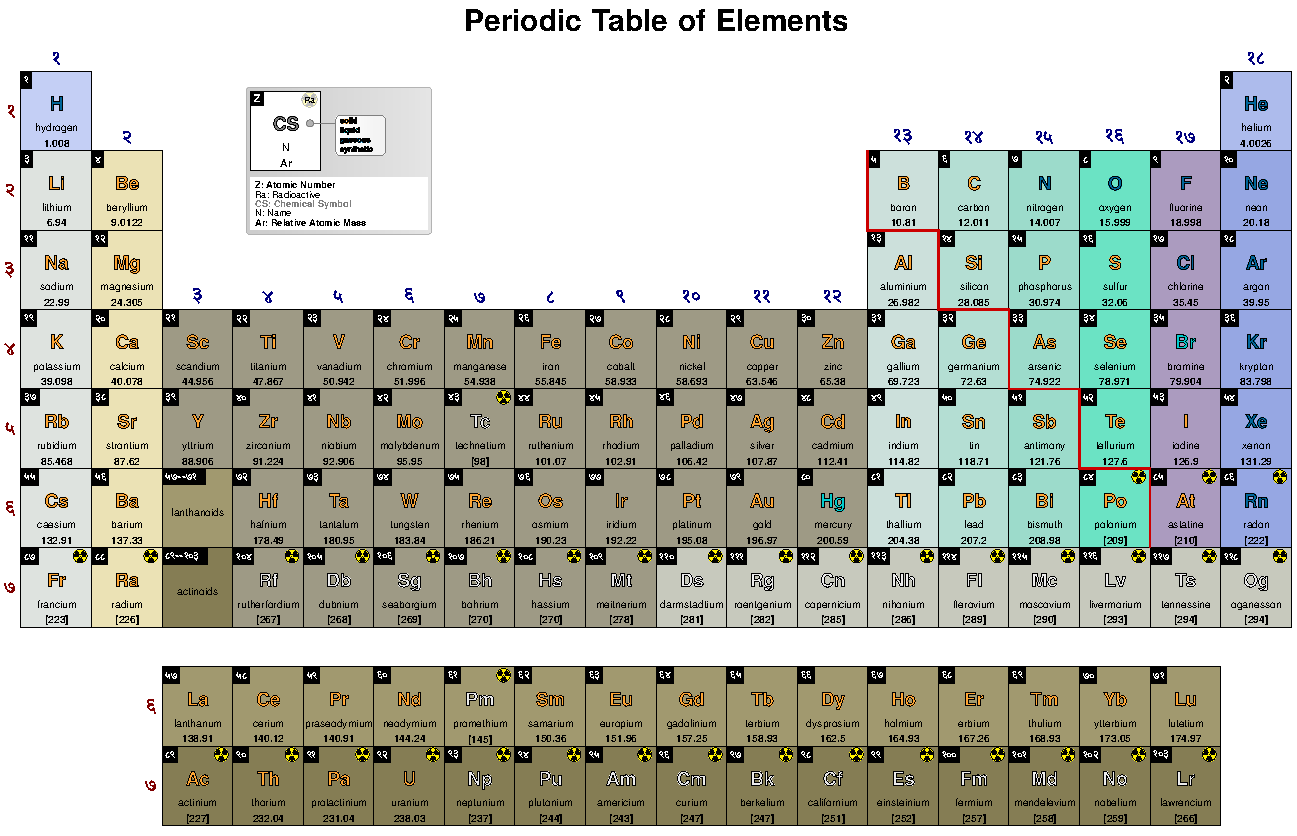
\includegraphics{manualfiles/pgfPTnumDeva.pdf}}}%
\\ [3pt]\pgfPTMline
\\ [6pt]It is also possible to load a font for the Devanagari numerals using the following command:
\index{COMMANDS@\textbf{COMMANDS}!\textbackslash pgfPTdvnfont}%
\\ [3pt]\bs{pgfPTdvnfont}\lp\red{font options}\rp\lb\red{font name}\rb
\\ [3pt]The default font is \textit{Eczar}.
\vfill
\subsubsection{Mandarin numerals}
To get some numbers of the Periodic Table with Mandarin numerals (the atomic number and the numeration of periods and groups) the package must be loaded with the above option \textit{numerals} set to \textbf{zh}:
\\ [3pt]\texttt{\large\textcolor{green!40!black}{\textbackslash usepackage}\textcolor{blue!70!black}{[}\textcolor{brown!60!black}{numerals=zh}%
\textcolor{blue!70!black}{]}\textcolor{purple!70!black}{\{}\textcolor{blue!70!black}{pgf-PeriodicTable}\textcolor{purple!40!black}{\}}}
\\ [6pt]\tikz{\node[text width=\linewidth-6mm,draw=orange!70,rounded corners=2pt,fill=black!10!orange!10,inner sep=3mm] {
This option works with the \textrm{Xe\LaTeX} and \textrm{Lua\LaTeX} engines to typeset the document and requires the \texttt{\large zhnumber} package, which is automatically loaded.};}
\newpage%\\ [10pt]
\tikz{\node[text width=\linewidth-8pt,inner xsep=4pt,align=left,fill=black!10,rounded corners=2pt] %
{\small\textcolor{black!50}{\%\ \string\usepackage[numerals=zh]\{pgf-PeriodicTable\}}};}%
\\ [-4pt]\pgfPTMmacrobox{pgfPT}[]%
\\ [10pt]\makebox[\linewidth][c]{\scalebox{.6}{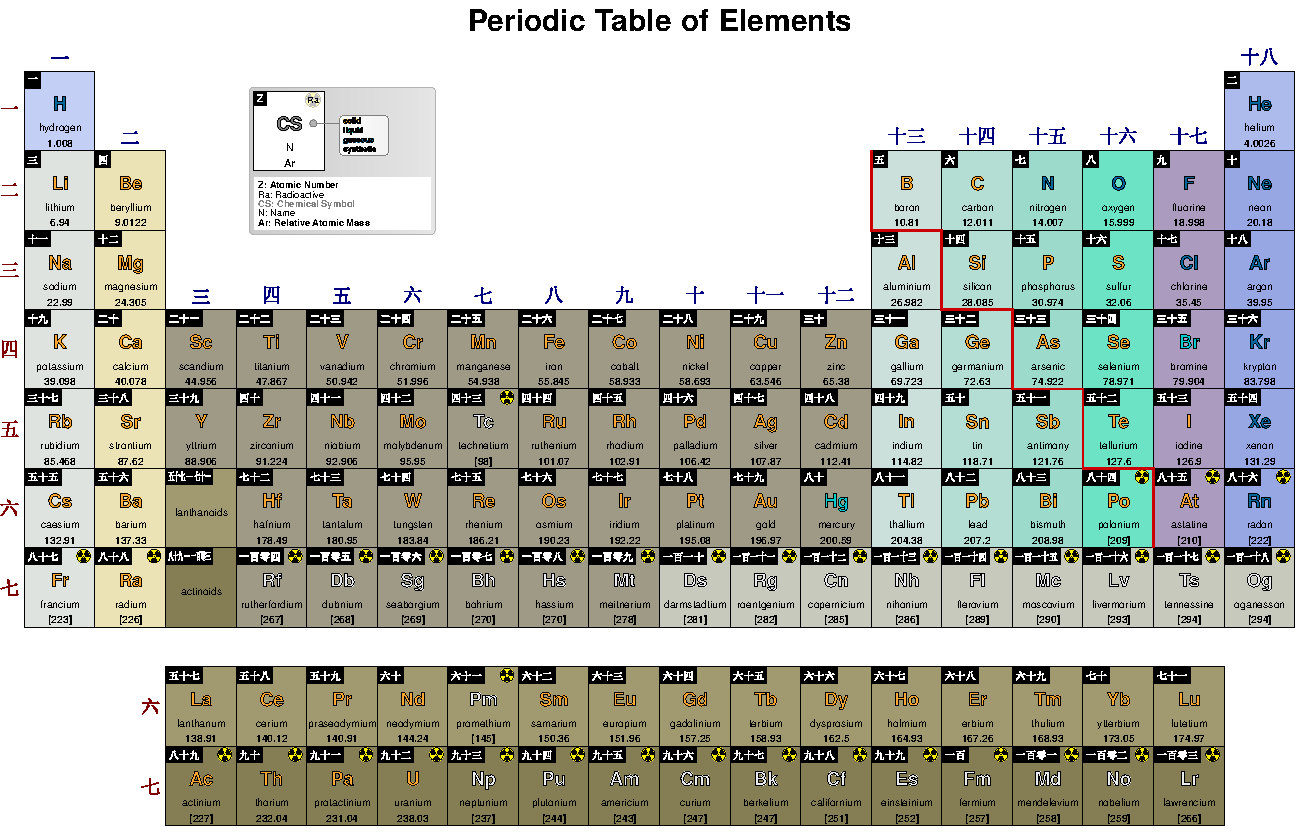
\includegraphics{manualfiles/pgfPTnumMand1.pdf}}}%
\\ [3pt]\pgfPTMline
\\ [6pt]As with the Devanagari numerals, the following command loads the specified font for the Mandarin numerals:
\index{COMMANDS@\textbf{COMMANDS}!\textbackslash pgfPTzhnumberfont}%\pgfPTzhnumberfont
\\ [3pt]\bs{pgfPTzhnumberfont}\lp\red{font options}\rp\lb\red{font name}\rb
\\ [3pt]\textit{For backwards compatibility (up to v2.1.4) the previous \bs{pgfPTzhfont} command now points to \bs{pgfPTzhnumberfont}, so older documents do not need any changes}.
\\ [3pt]The default font is \textit{BabelStone Han} (since v2.1.5) loaded with the \textit{AutoFakeBold=4} option. For details on installing this font, see the \hyperlink{subsec::zhLang}{Chinese (zh) subsection} below.
\\ [6pt]It is also possible to enable or disable the numbers shown in Mandarin with the command:
\\ [3pt]\bs{pgfPTzhnumber}\lp\red{<true|false>}\rp\lb\red{comma separated list}\rb
\\ [3pt] The list can have \red{Z} for the atomic number, \red{per} for the period numbers and \red{gr} for the group numbers. At package loading, with this option, they are set to \red{true}.
\index{COMMANDS@\textbf{COMMANDS}!\textbackslash pgfPTzhnumber}%
\\ [10pt]\tikz{\node[text width=\linewidth-8pt,inner xsep=4pt,align=left,fill=black!10,rounded corners=2pt] %
{\small\textcolor{black!50}{\%\ \string\usepackage[numerals=zh]\{pgf-PeriodicTable\}}};}%
\\ [-4pt]\tikz{\node[text width=\linewidth-8pt,inner xsep=4pt,align=center,fill=black!10,rounded corners=2pt] %
{\bs{pgfPTzhnumber}\lp\red{false}\rp\lb\red{Z}\rb};}%
\\ [-4pt]\pgfPTMmacrobox{pgfPT}[Z list={1,...,36}]%
\\ [10pt]\makebox[\linewidth][c]{\scalebox{.6}{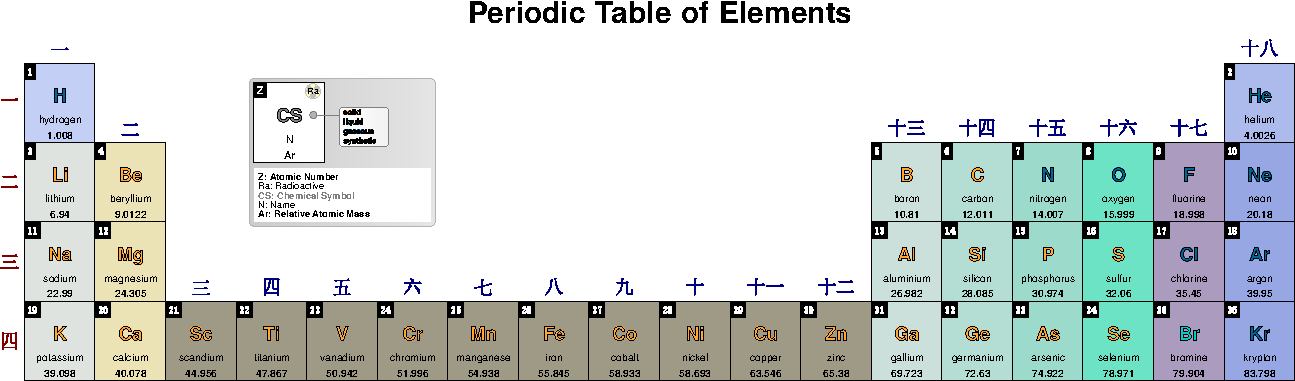
\includegraphics{manualfiles/pgfPTnumMand2.pdf}}}%
\\ [3pt]\pgfPTMline
\newpage%
\subsection{User languages}
\textit{User languages} are provided by user translations. They are only available if passed as an option when loading the package. In addition to the \textit{built-in} languages, the chosen language is the only one available and becomes the default language for the Periodic Table.
\bigskip
\subsubsection{Dutch (nl)}
The Dutch language is loaded by:
\\ [3pt]\texttt{\large\textcolor{green!40!black}{\textbackslash usepackage}\textcolor{blue!70!black}{[}\textcolor{brown!60!black}{userlang=nl}%
\textcolor{blue!70!black}{]}\textcolor{purple!70!black}{\{}\textcolor{blue!70!black}{pgf-PeriodicTable}\textcolor{purple!40!black}{\}}}
\\ [10pt]\tikz{\node[text width=\linewidth-8pt,inner xsep=4pt,align=left,fill=black!10,rounded corners=2pt] %
{\small\textcolor{black!50}{\%\ \string\usepackage[userlang=nl]\{pgf-PeriodicTable\}}};}%
\\ [-4pt]\pgfPTMmacrobox{pgfPT}[]%
\\ [10pt]\makebox[\linewidth][c]{\scalebox{.6}{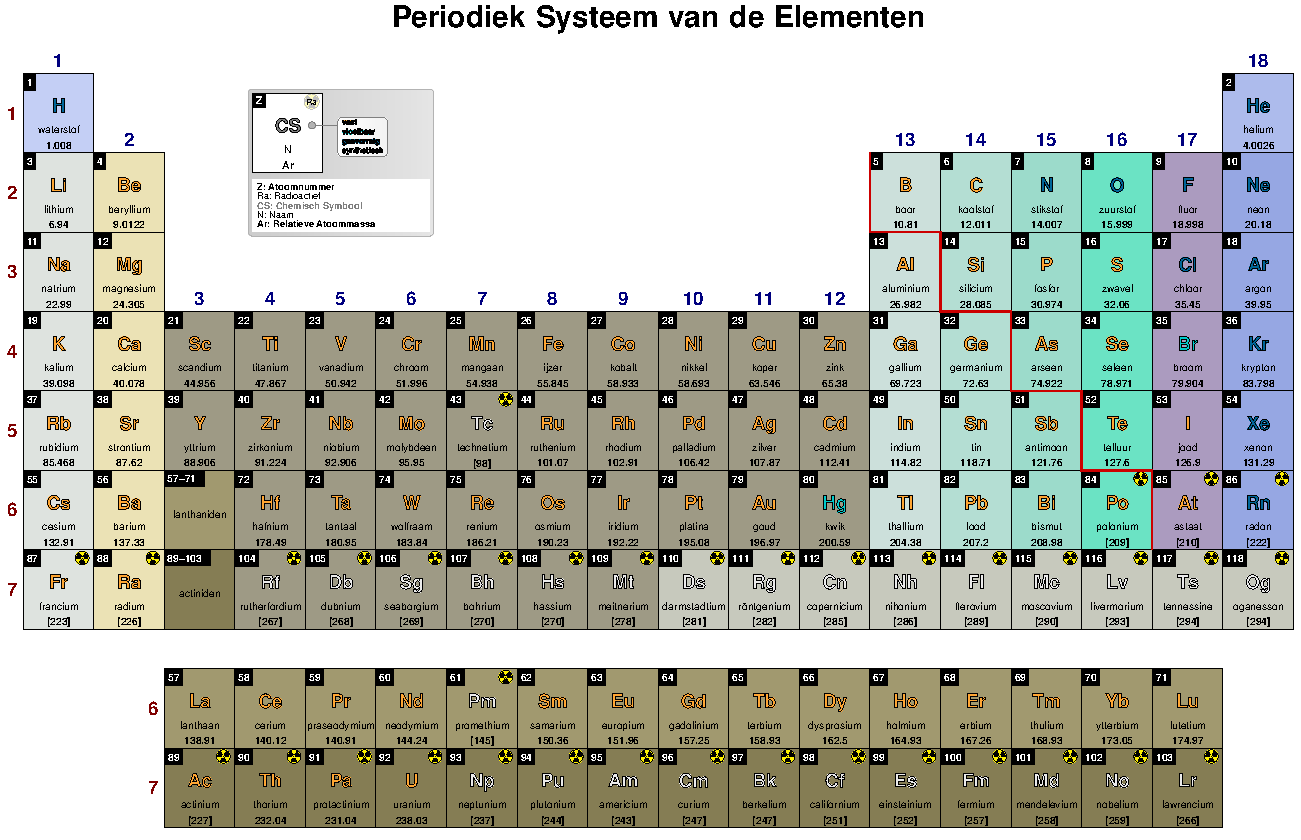
\includegraphics{manualfiles/pgfPT_nl.pdf}}}%
\\ [3pt]\pgfPTMline
\bigskip
\subsubsection{Chinese (zh)}
\hypertarget{subsec::zhLang}{The Chinese language} is loaded by:
\\ [3pt]\texttt{\large\textcolor{green!40!black}{\textbackslash usepackage}\textcolor{blue!70!black}{[}\textcolor{brown!60!black}{userlang=zh}%
\textcolor{blue!70!black}{]}\textcolor{purple!70!black}{\{}\textcolor{blue!70!black}{pgf-PeriodicTable}\textcolor{purple!40!black}{\}}}
\\ [6pt]\tikz{\node[text width=\linewidth-6mm,draw=orange!70,rounded corners=2pt,fill=black!10!orange!10,inner sep=3mm] {%
The default font is \textit{BabelStone Han} \textbf{which is not available in TeX Live}.
\\ It can be downloaded for free from the BabelStone website:
\\ [3pt]\hfil\href{https://www.babelstone.co.uk/Fonts/Han.html}{https://www.babelstone.co.uk/Fonts/Han.html}\hfil};}
\\ [6pt]The use of a font which is not included in the TeX Live software distribution, nor in common Operating Systems, circumvents the missing Ideographs for the most recent elements -- from rutherfordium to oganesson. The BabelStone Han has all of them as can be seen in the following table:
\begin{center}\small
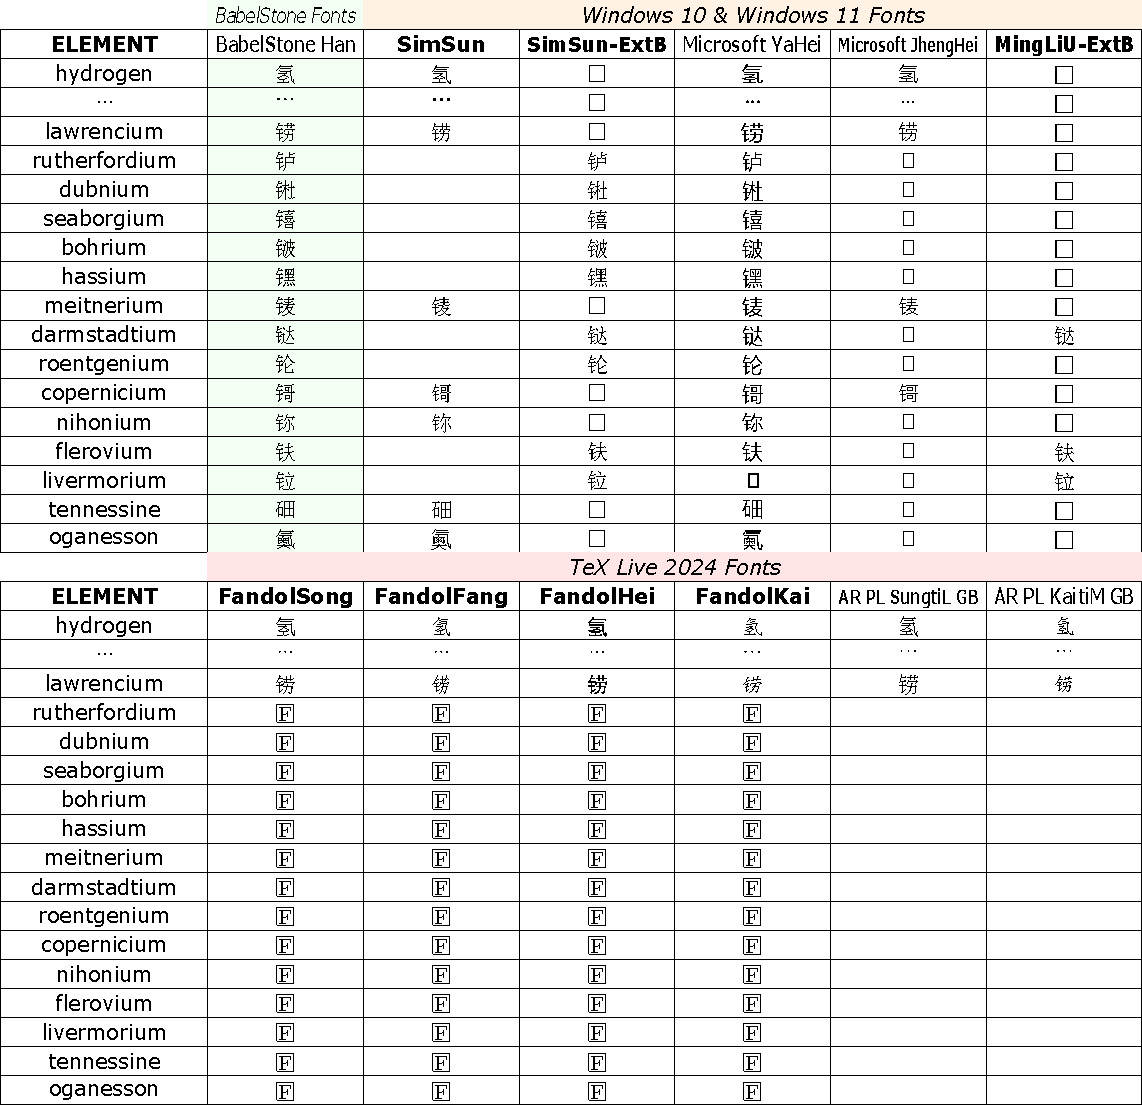
\includegraphics[width=\linewidth]{manualfiles/pgfPT_zh_fonts.pdf}
\\ [3pt]Glyphs available in \textsf{BabelStone Han} font and in some Windows and TeX Live fonts.
\end{center}
\vfill%
To use the BabelStone Han it is necessary to \href{https://www.babelstone.co.uk/Fonts/Download/BabelStoneHan.zip}{download it}, unzip it and install the extracted font file:
\begin{itemize}\small
\item for Windows users, just right click on \textsf{BabelStoneHan.ttf} and choose \textsf{install for all users}. This can also be done in Windows Settings $\rightarrow$ Personalization $\rightarrow$ Fonts.
\item for Linux users, open the Linux Terminal and type \textsf{sudo apt install fonts-BabelStoneHan.ttf}
\item for macOS users, just copy or drag the font file (\textsf{BabelStoneHan.ttf}) into \textsf{/Library/Fonts} or \mbox{double-click} on \textsf{BabelStoneHan.ttf} to open the preview window. Click on \textsf{Install font} button at the bottom of the preview window.
\end{itemize}\medskip
Make sure the \textsf{BabelStone Han} font is \textit{visible} to the \textrm{Xe\LaTeX} or \textrm{Lua\LaTeX} engines.
\\ [9pt]If you do not want to install this font on your operating system, you can place it in the \textsf{truetype} fonts folder in the TeX Live distribution and \textit{Update filename database} in the TeX Live manager. After that, the font will be known only by the filename \textsf{BabelStoneHan.ttf} instead of its name, \textsf{BabelStone Han}.

\newpage%
\tikz{\node[text width=\linewidth-8pt,inner xsep=4pt,align=left,fill=black!10,rounded corners=2pt] %
{\small\textcolor{black!50}{\%\ \string\usepackage[userlang=zh]\{pgf-PeriodicTable\}}};}%
\\ [-4pt]\pgfPTMmacrobox{pgfPT}[]%
\\ [10pt]\makebox[\linewidth][c]{\scalebox{.6}{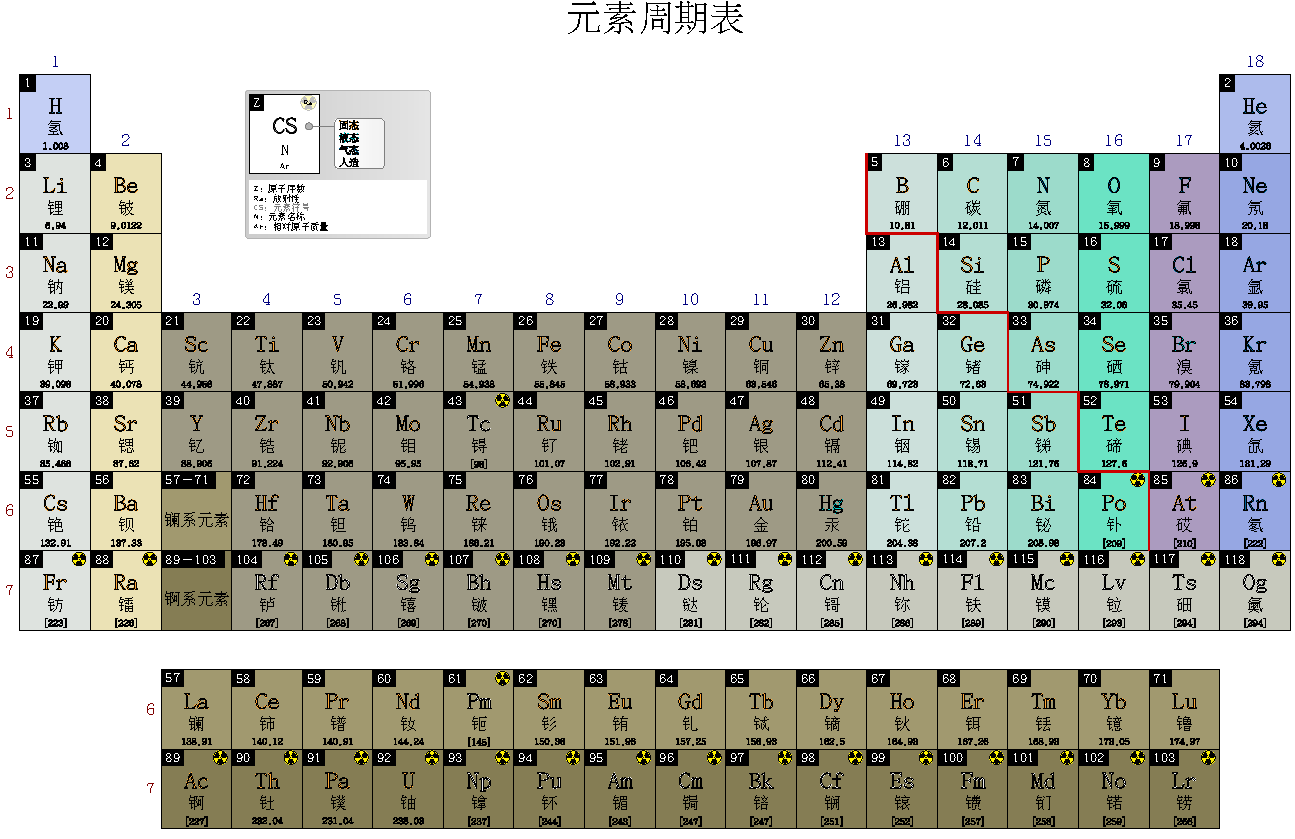
\includegraphics{manualfiles/pgfPT_zh_1.pdf}}}%
\\ [3pt]\pgfPTMline
\vfill
To get the Periodic Table with the atomic number and the period/group numbers in mandarin numerals load the package with the correponding options:
\\ [10pt]\tikz{\node[text width=\linewidth-8pt,inner xsep=4pt,align=left,fill=black!10,rounded corners=2pt] %
{\small\textcolor{black!50}{\%\ \string\usepackage[userlang=zh,numerals=zh]\{pgf-PeriodicTable\}}};}%
\\ [-4pt]\pgfPTMmacrobox{pgfPT}[]%
\\ [10pt]\makebox[\linewidth][c]{\scalebox{.6}{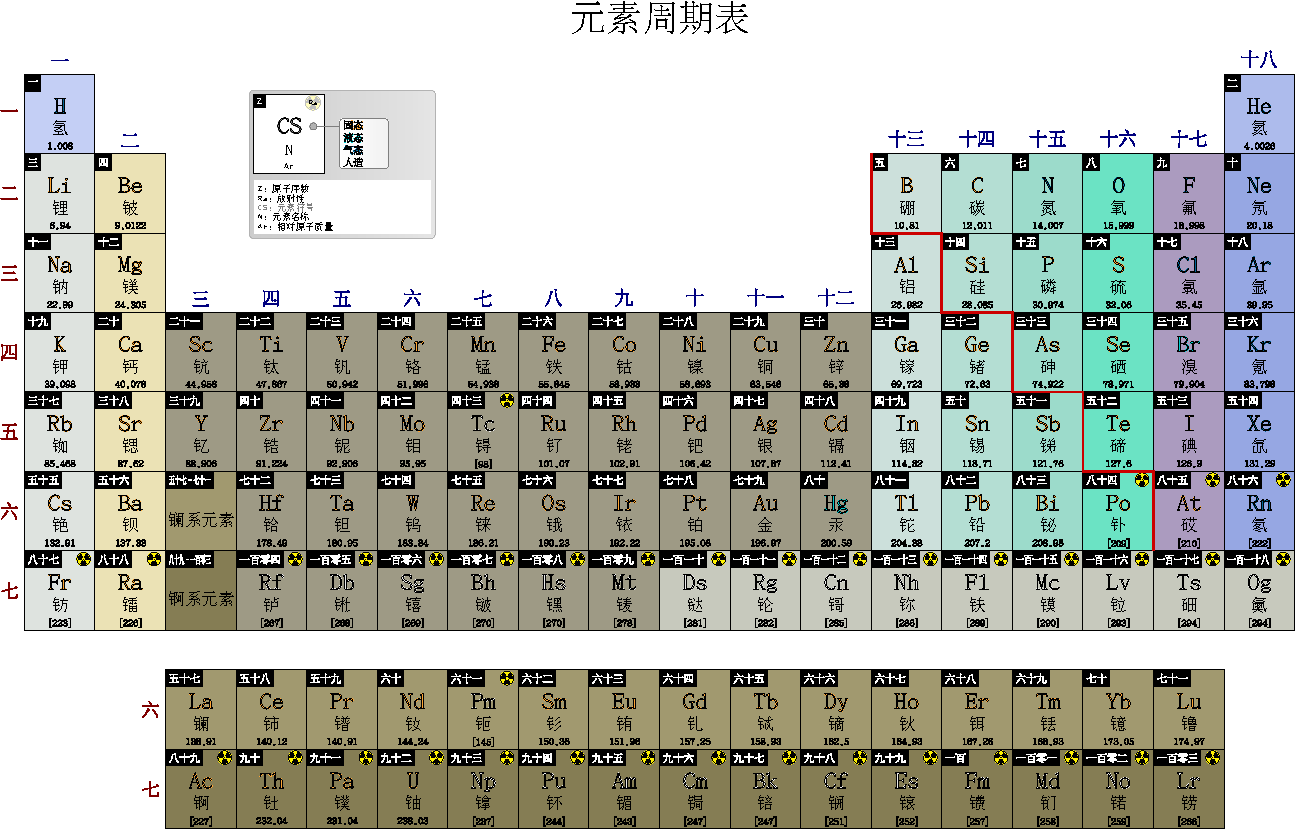
\includegraphics{manualfiles/pgfPT_zh_2.pdf}}}%
\\ [3pt]\pgfPTMline
\newpage%
When the Chinese language is loaded four extra commands are defined:
\begin{itemize}
\item\bs{pgfPTzhFontFeatures}\index{COMMANDS@\textbf{COMMANDS}!\textbackslash pgfPTzhFontFeatures} can be used to set font features for the loaded Chinese font (set by the \red{font} option). For more details see the \textsf{fontspec} package documentation.
\item\bs{pgfPTzhtextfontSS}\index{COMMANDS@\textbf{COMMANDS}!\textbackslash pgfPTzhtextfontSS} is used to set the font for the elements meitnerium, copernicium, nihonium, tennessine and oganesson (Z=109, 112. 113, 117 and 118).
\item\bs{pgfPTzhtextfontSSB}\index{COMMANDS@\textbf{COMMANDS}!\textbackslash pgfPTzhtextfontSSB} is used to set the font for the elements rutherfordium, dubnium, seaborgium, bohrium, hassium,darmstadtium, roentgenium and flerovium (Z=104, 105, 106, 107, 108, 110, 111 and 114).
\item\bs{pgfPTzhtextfontLv}\index{COMMANDS@\textbf{COMMANDS}!\textbackslash pgfPTzhtextfontLv} is used to set the livermorium (Z=116) font.
\end{itemize}
The defaults for some features of the Periodic Table are also changed:
\begin{itemize}
\item[--]the \red{name font} is switched from \texttt{\large\textbackslash tiny} to \texttt{\large\textbackslash footnotesize}.
\item[--]the \red{CS font} is switched from \texttt{\large\textbackslash small\textbackslash bfseries} to \texttt{\large\textbackslash large}.
\item[--]the \red{title font} is switched from \texttt{\large\textbackslash Large\textbackslash bfseries} to \texttt{\large\textbackslash LARGE}.
\item[--]when not using the Chinese numerals (loaded with the option \textcolor{brown!60!black}{numerals=zh}) the \red{Z font} is switched from \texttt{\large\textbackslash tiny\textbackslash bfseries} to \texttt{\large\textbackslash scriptsize}, as well the \red{Z padding} is changed from \texttt{\large 0.25ex} to \texttt{\large 0ex}.
\end{itemize}
\tikz{\node[text width=\linewidth-8pt,inner xsep=4pt,align=left,fill=black!10,rounded corners=2pt] %
{\small\textcolor{black!50}{\%\ \string\usepackage[userlang=zh]\{pgf-PeriodicTable\}}};}%
\\ [-4pt]\tikz{\node[text width=\linewidth-8pt,inner xsep=4pt,align=left,fill=black!10,rounded corners=2pt,text=black!50] %
{\bs{pgfPTzhtextfontSS}\lb\red{SimSun}\rb\% font for Z=\{109,112.113,117,118\}
\\ \makebox[8em][s]{}\% meitnerium, copernicium, nihonium, tennessine, oganesson
\\ \bs{pgfPTzhtextfontSSB}\lb\red{SimSun-ExtB}\rb\% font for
\\ \makebox[8em][s]{}\% Z=\{104,105,106,107,108,110,111,114\}
\\ \makebox[8em][s]{}\% rutherfordium, dubnium, seaborgium, bohrium, hassium,
\\ \makebox[8em][s]{}\% darmstadtium, roentgenium, flerovium
\\ \bs{pgfPTzhtextfontLv}\lb\red{SimSun-ExtB}\rb\% font for Z=116
\\ \makebox[8em][s]{}\% livermorium
};}%
\\ [-4pt]\pgfPTMmacrobox[l]{pgfPT}[font=SimSun]%
\\ [10pt]\makebox[\linewidth][c]{\scalebox{.6}{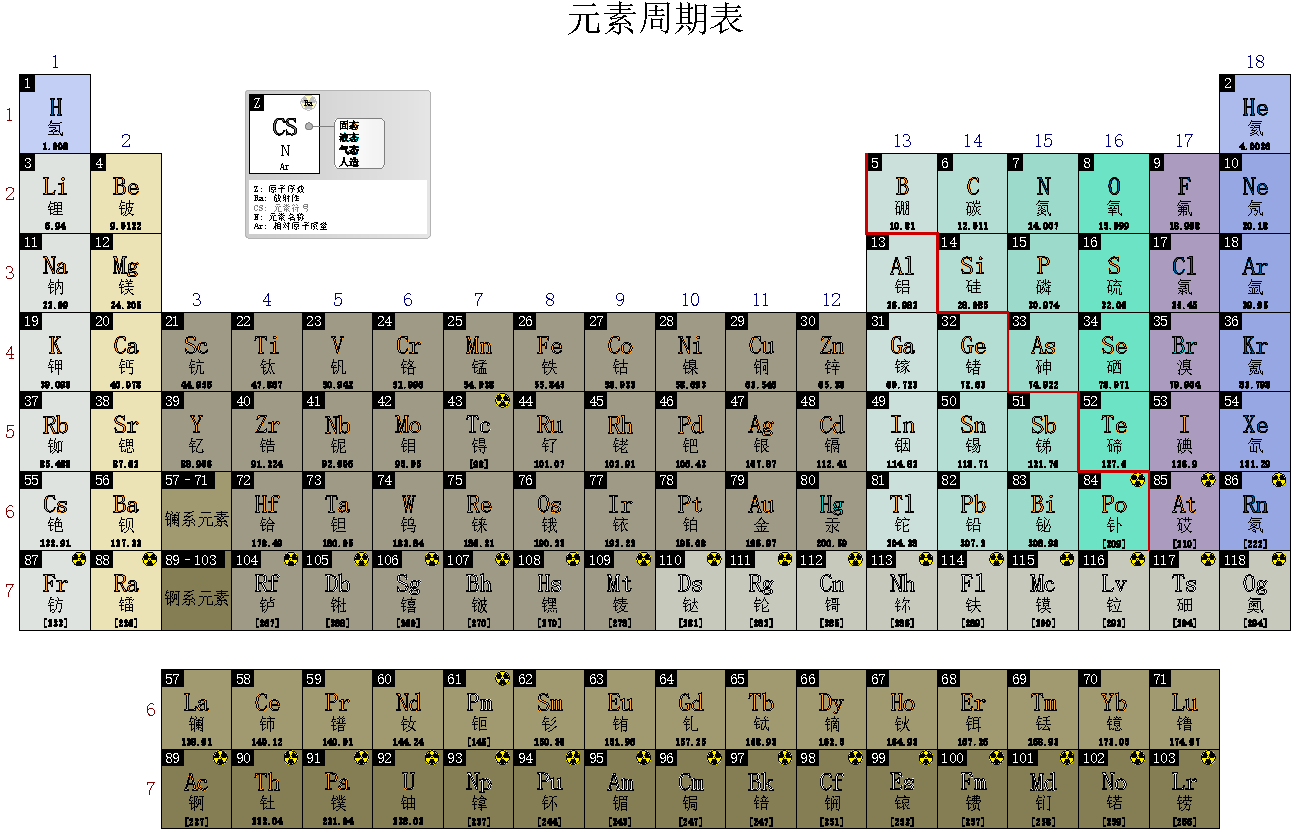
\includegraphics{manualfiles/pgfPT_zh_3.pdf}}}%
\\ [3pt]\pgfPTMline
\newpage%
\subsection{Interaction with other packages}
\subsubsection{fontspec}
To correctly set the font in each cell contents the command \bs{fontspec} must be used. For example if you want to use \textit{Arial} for the \red{name font}, it must be set using \red{name font=\bs{fontspec}\lb Arial\rb\bs{selectfont}}.\\ All other font selection commands, \eg, \bs{large}, \mbox{\bs{itshape}}, are used as usual. For example if you want to use \textit{Arial}\hfil\ in\hfil\ \textit{large}\hfil\ size\hfil\ and\hfil\ \textit{bold}\hfil\ weight\hfil\ for\hfil\ the \red{name font}, then you type
\\ \makebox[\linewidth][s]{\red{name font=\bs{large}\bs{bfseries}\bs{fontspec}\lb Arial\rb\bs{selectfont}}\hfil\ or\hfil\  \red{name font=\bs{fontspec}\lb Arial\rb}}
\\ \bs{large}\bs{bfseries}\bs{selectfont}.
\subsubsection{ragged2e}
Using \texttt{\large\textcolor{green!40!black}{\textbackslash usepackage}\textcolor{blue!70!black}{[}\textcolor{brown!60!black}{document}%
\textcolor{blue!70!black}{]}\textcolor{purple!70!black}{\{}\textcolor{blue!70!black}{ragged2e}\textcolor{purple!40!black}{\}}} and \texttt{\large\textcolor{green!40!black}{\textbackslash usepackage}%
\textcolor{purple!70!black}{\{}\textcolor{blue!70!black}{pgf-PeriodicTable}\textcolor{purple!40!black}{\}}} together, the Periodic Table will be completely fractured and out of the page.
\\ [6pt]\textit{Solution}:
\vspace{4pt}\hrule\vspace{4pt}Use a local group: \{\bs{justifying}\bs{pgfPT}\}\vspace{4pt}\hrule%
\subsubsection{beamer}
\textrm{\large beamer}, \pack{} and \textrm{PDF\LaTeX} in combination have an issue: the \texttt{\large\textbackslash textsc} fails to produce the correct small caps. The error given is:
\smallskip\hrule\begin{verbatim}
Font shape `T1/cmss/m/sc' undefined
(Font) using `T1/cmss/m/n' instead on input line ...
\end{verbatim}\hrule
\smallskip\hrule\smallskip\bigskip
To avoid this, the \pack{} package can be loaded with one of the following options:
\begin{description}
\item[\red{beamer}] which loads the \textrm{\large lmodern} package, setting small caps compatibility with beamer via `lmodern' package.
\\ \tikz{\node[text width=\linewidth-8pt,inner xsep=4pt,align=left,fill=black!10,rounded corners=2pt] %
{\small\textcolor{black!50}{\%\ \string\usepackage[beamer]\{pgf-PeriodicTable\}}};}%
\item[\red{beamer*}] which sets small caps compatibility with beamer via T1 \textrm{\large cmr} fonts.
\\ \tikz{\node[text width=\linewidth-8pt,inner xsep=4pt,align=left,fill=black!10,rounded corners=2pt] %
{\small\textcolor{black!50}{\%\ \string\usepackage[beamer*]\{pgf-PeriodicTable\}}};}%
\item[\red{beamer**}] which sets small caps compatibility with beamer via T1 \textrm{\large cmr} fonts and loads the \textrm{\large silence} package to suppress small caps font substitution warnings.
\\ \tikz{\node[text width=\linewidth-8pt,inner xsep=4pt,align=left,fill=black!10,rounded corners=2pt] %
{\small\textcolor{black!50}{\%\ \string\usepackage[beamer**]\{pgf-PeriodicTable\}}};}%
\end{description}
\newpage
\section{The data}
The data available in \pack{} was mainly compiled with selected and filtered data from Wikipedia, taken from November 2021 to July 2022.
\\ [12pt]\header
\\ [-1pt]\linhaimpar{Ar}{Relative Atomic Mass}{}{(Wikidata @09/jan/2022)}%
\\ [-1pt]\linhapar{Arstar}{Standard Relative\newline Atomic Mass}{}{ STANDARD ATOMIC WEIGHTS 2021, %
Commission on Isotopic Abundances and Atomic Weights,\newline\bfseries\textsf{\textcopyright} CIAAW, 2007--2022%
\newline(\href{https://ciaaw.org/impressum.htm}{https://ciaaw.org/impressum.htm})}%
\\ [-1pt]\linhaimpar{radio}{Radioactivity}{}{(gperiodic-3.0.3, Dec 26 2018)}%
\\ [-1pt]\linhapar{R}{Atomic Radius}{$\mathsf{pm}$}{Calculated (Wikidata @04/jul/2022)}%
\\ [-1pt]\linhaimpar{Rcov}{Covalent Radius}{$\mathsf{pm}$}{Single bond, Wikidata @04/jul/2022)}%
\\ [-1pt]\linhapar{Rion}{Ionic Radius}{$\mathsf{pm}$}{(Wikidata @04/jul/2022)}%
\\ [-1pt]\linhaimpar{Ei}{First Ionization Energy}{$\mathsf{kJ\cdot mol^{-1}}$}{(Wikidata @04/jul/2022)}%
\\ [-1pt]\linhapar{eneg}{Electronegativity\newline (Pauling)}{}{(Wikidata @04/jul/2022)}%
\\ [-1pt]\linhaimpar{eaff}{Electroaffinity}{$\mathsf{kJ\cdot mol^{-1}}$}{(Wikidata @04/jul/2022)}%
\\ [-1pt]\linhapar{O}{Oxidation States}{}{(Wikidata @09/jan/2022)}%
\\ [-1pt]\linhaimpar{Tmelt}{Melting Point}{$\mathsf{K}$}{at standard pressure (Wikidata @21/dez/2021)}%
\\ [-1pt]\linhapar{TmeltC}{Melting Point}{$\mathsf{^oC}$}{at standard pressure (Wikidata @21/dez/2021)}%
\\ [-1pt]\linhaimpar{Tboil}{Boiling Point}{$\mathsf{K}$}{at standard pressure (Wikidata @21/dez/2021)}%
\\ [-1pt]\linhapar{TboilC}{Boiling Point}{$\mathsf{^oC}$}{at standard pressure (Wikidata @21/dez/2021)}%
\\ [-1pt]\linhaimpar{eDist}{Electron Distribution}{}{(Wikidata @01/nov/2021)}%
\\ [-1pt]\linhapar{eConfign}{Electronic Configuration (increasing n)}{}{(Wikidata @01/nov/2021)}%
\\ [-1pt]\linhaimpar{eConfignl}{Electronic Configuration (increasing $\mathsf{n+\ell}$)}{}{(Wikidata @01/nov/2021)}%
\\ [-1pt]\linhapar{d}{Density}{$\mathsf{g\cdot dm^{-3}}$ {\tiny for gases}\newline$\mathsf{g\cdot cm^{-3}}$ {\tiny all other physical states}}{physical state at $\mathsf{25^oC, 1\,atm}$ (Wikidata @01/nov/2021)}%
\\ [-1pt]\linhaimpar{Cp}{Specific heat capacity}{$\mathsf{J\cdot mol^{-1}\cdot K^{-1}}$}{at $\mathsf{25^oC}$ and $\mathsf{100\,kPa}$ (Wikidata @20/nov/2021)}%
\\ [-1pt]\linhapar{kT}{Thermal Conductivity}{$\mathsf{W\cdot m^{-1}\cdot K^{-1}}$}{at $\mathsf{25^oC}$ (Wikidata @21/nov/2021)}%
\\ [-1pt]\linhaimpar{ls}{Lattice Structure}{}{(Wikidata @20/dez/2021 and \href{http://wwwhomes.uni-bielefeld.de/achim/ele_structures.html}{University of Bielefeld})}%
\\ [-1pt]\linhapar{lsa}{Lattice constant: a}{$\mathsf{pm}$}{(University of Bielefeld @21/dez/2021)}%
\\ [-1pt]\linhaimpar{lsb}{Lattice constant: b}{$\mathsf{pm}$}{(University of Bielefeld @21/dez/2021)}%
\\ [-1pt]\linhapar{lsc}{Lattice constant: c}{$\mathsf{pm}$}{(University of Bielefeld @21/dez/2021)}%
\\ [-1pt]\linhaimpar{lsca}{Lattice c/a ratio}{}{Calculated from available data and rounded to two digits}%
\\ [-1pt]\linhapar{DiscY}{Discover Year}{}{(Wikidata @22/dez/2021)}%
\\ [-1pt]\linhaimpar{DiscC}{Discover Country}{}{(Wikidata @22/dez/2021)}%
\\ [-1pt]\linhapar{spectra}{Visible range spectral lines}{}{Elements spectrum made with \textcolor{blue!50!black}{\textbackslash pgfspectra}.\newline See the \footnotesize\href{https://ctan.org/pkg/pgf-spectra}{\textsf{pgf-spectra}}\scriptsize\ manual for more details}%
\\ [12pt]The utilization of the \textit{acronyms} will be explained in \hyperlink{secBuildCell}{Designing cells with \textbackslash pgfPTbuildcell}.
\vfill\vfill\vfill\newpage
%%%%%%%%%%%%%%%%%%%%%%%%%%%%%%%%%%%%%%%%%%%%%%%%%%%%%%%%%%%%
\label{file:commands}%
\section{The commands}
\hypertarget{sec:com}{The} commands to achieve the Periodic Table of Elements are:
\begin{itemize}
\item\pgfPTMmacro{pgfPT}[]\ or \pgfPTMmacro{pgfPT}[options list] -- draws a full or partial graphical Periodic Table controlled by the optional keys.
\item\pgfPTMmacro{pgfPTstyle}[options list] -- sets the global style for the Periodic Table.
\item\pgfPTMmacro{pgfPTresetstyle}[] -- resets the style for the Periodic Table with the default values.
\item\pgfPTMmacro{pgfPTbuildcell}[]\blue{(}\textcolor{red!50!black}{nrows,ncolumns}\blue{)}\lp\red{entries}\rp%
\ -- builds the contents of each cell in the Periodic Table.
\item\pgfPTMmacro{pgfPTresetcell}[] -- resets the cell to its default layout.%
\item\pgfPTMmacro{pgfPTbuildcellstyle}[]\lb\red{name}\rb\blue{(}\red{nrows,ncolumns}\blue{)}\lp\red{entries}\rp%
\ -- builds the contents of each cell in the Periodic Table and stores it in a named style.
%\item\pgfPTMmacro{showcellinfo}[] -- shows the information about the contents of the last unnamed builded cell. If no cells have yet been build, the default cell is shown.
%\item\pgfPTMmacro{showcellstyleinfo}[]\textcolor{blue!50!black}{(}\textcolor{red!50!black}{name}\textcolor{blue!50!black}{)} -- shows the information about the contents of the named builded cell.
\item\pgfPTMmacro{pgfPTpreviewcell}[]\ or \pgfPTMmacro{pgfPTpreviewcell}[scale factor] -- preview the last unnamed built cell with an optional scale factor. If no cells have yet been built, the default cell is shown.
\item\pgfPTMmacro{pgfPTpreviewcellstyle}[]\lb\red{name}\rb%
\ or \pgfPTMmacro{pgfPTpreviewcellstyle}[]\lp\red{scale factor}\rp\lb\red{name}\rb%
\ -- preview the named builded cell with an optional scale factor.
\item\pgfPTMmacro{pgfPTnewColorScheme}[trailing color]\lb\red{name}\rb\lb\red{color list}\rb%
\ -- makes a color scheme to fill the cells along the Periodic Table.
\item\pgfPTMmacro{pgfPTnewZlist}[]\lb\red{name}\rb%
\ -- create a user defined atomic numbers (Z) \red{named} list.
\item\pgfPTMmacro{pgfPTsetLanguage}[]\lb\red{language flag}\rb%
\ -- globally change the default language.
\end{itemize}
\vspace{-32pt}\ %
\def\tmpSection{\bs{pgfPT}}%
\subsection*{}{\normalfont\large\bfseries\raisebox{1.25pt}{$\mathbf{\blacktriangleright}$}\ Utilization of \tmpSection}%
\label{command:pgfPT}\addcontentsline{toc}{subsection}{\texorpdfstring{\tmpSection{}}{\textbackslash pgfPT}}%
\index{COMMANDS@\textbf{COMMANDS}!\textbackslash pgfPT}%
\\ [4pt]Use this command to draw the Periodic Table of Elements in the language selected at package inclusion (\texttt{\large\textcolor{green!40!black}{\textbackslash usepackage}\textcolor{blue!70!black}{[}\textcolor{brown!60!black}{language flag}\textcolor{blue!70!black}{]}\textcolor{purple!70!black}{\{}\textcolor{blue!70!black}{pgf-PeriodicTable}\textcolor{purple!40!black}{\}}}):
\\ [5pt]\pgfPTMmacrobox{pgfPT}[]%
\\ [10pt]\makebox[\linewidth][c]{\scalebox{.6}{\pgfPT}}%
\\ [0pt]\pgfPTMline%
\newpage%
This command can also be used with options -- as described in section \hyperlink{OPTIONS}{Options for \textbackslash pgfPT: creating a �Periodic Table�} -- to modify, for instance, the font of the Periodic Table or the colors of the cells:
\\ [10pt]\pgfPTMmacrobox{pgfPT}[font=pnc,back color scheme=pgfPTMNM]%
\\ [10pt]\makebox[\linewidth][c]{\scalebox{.6}{\pgfPT[font=pnc,back color scheme=pgfPTMNM]}}%
\\ [0pt]\pgfPTMline%
%%%%%%%%%%%%%%%%%%%%%%%%%%%%%%%%%%%%%%%%%%%%%%%%%%%%%%%%%%%%
\\ [-32pt]\ %
\def\tmpSection{\bs{pgfPTstyle}\lp\red{options list}\rp}%
\subsection*{}{\normalfont\large\bfseries\raisebox{1.25pt}{$\mathbf{\blacktriangleright}$}\ Utilization of \tmpSection}%
\label{command:pgfPTstyle}\addcontentsline{toc}{subsection}{\texorpdfstring{\tmpSection{}}{\textbackslash pgfPTstyle}}%
\index{COMMANDS@\textbf{COMMANDS}!\textbackslash pgfPTstyle}%
\\ [4pt]This command globally sets a style for the Periodic Table:
\\ [10pt]\pgfPTMmacrobox[l]{pgfPTstyle}[font=ptm,IUPAC=false,show title=false]%
\pgfPTstyle[font=ptm,IUPAC=false,show title=false]%
\\ [-4pt]\pgfPTMmacrobox{pgfPT}[]%
\\ [10pt]\makebox[\linewidth][c]{\scalebox{.6}{\pgfPT}}%
\\ [0pt]\pgfPTMline%
\newpage%\\ [5pt]
It is possible to locally override the \textit{global style} defined:
\\ [5pt]\pgfPTMmacrobox{pgfPT}[show title]%
\\ [10pt]\makebox[\linewidth][c]{\scalebox{.6}{\pgfPT[show title]}}%
\\ [5pt]\pgfPTMline%
%%%%%%%%%%%%%%%%%%%%%%%%%%%%%%%%%%%%%%%%%%%%%%%%%%%%%%%%%%%%
%\newpage\ \\ [-62pt]%
\\ [-32pt]\ %
\def\tmpSection{\bs{pgfPTresetstyle}}%
\subsection*{}{\normalfont\large\bfseries\raisebox{1.25pt}{$\mathbf{\blacktriangleright}$}\ Utilization of \tmpSection}%
\label{command:pgfPTresetstyle}\addcontentsline{toc}{subsection}{\texorpdfstring{\tmpSection{}}{\textbackslash pgfPTresetstyle}}%
\index{COMMANDS@\textbf{COMMANDS}!\textbackslash pgfPTresetstyle}%
\\ [4pt]This command resets the style used in the Periodic Table to default values:
\\ [10pt]\pgfPTMmacrobox[l]{pgfPTresetstyle}[]%
\pgfPTresetstyle%
\\ [-4pt]\pgfPTMmacrobox{pgfPT}[]%
\\ [10pt]\makebox[\linewidth][c]{\scalebox{.6}{\pgfPT}}%
\\ [0pt]\pgfPTMline%
%%%%%%%%%%%%%%%%%%%%%%%%%%%%%%%%%%%%%%%%%%%%%%%%%%%%%%%%%%%%
\newpage\ \\ [-62pt]
%\\ [-32pt]\ %
\def\tmpSection{\bs{pgfPTbuildcell}\blue{(}\red{nrows,ncolumns}\blue{)}\lp\red{entries}\rp}%
\subsection*{}{\color{black}\normalfont\large\bfseries\raisebox{1.25pt}{$\mathbf{\blacktriangleright}$}\ Utilization of \tmpSection}%
\label{command:pgfPTbuildcell}\addcontentsline{toc}{subsection}{\texorpdfstring{\tmpSection{}}{\textbackslash pgfPTbuildcell}}%
\index{COMMANDS@\textbf{COMMANDS}!\textbackslash pgfPTbuildcell}%
\\ [4pt]With \pgfPTMmacro{pgfPTbuildcell}[] it is possible to customize the \textit{elementar} cell of the Periodic Table. Each cell is built on the given \textit{number of rows} and \textit{number of columns}. After that, each \textit{entry} is constructed according to the structure \red{row;column;what} or \red{initial row-final row;initial column-final column;what}.
\vspace{8pt}%
\begin{itemlist}
\item The first \textit{syntax} -- \red{row;column;what} -- puts �\red{what}� in the �\red{row}� row and in the �\red{column}� column with the height of one row and the width of one column:
\\ -- for example, \red{1;1;Z} puts the atomic number \red{Z} in row \red{1} and column \red{1}, witch actually corresponds to a box anchored to the top left corner of the cell and that \textit{goes} below and to the right of that corner.
\item The second \textit{syntax} -- \mbox{\red{initial row-final row;initial column-final column;what}} -- puts �\red{what}� from �\red{initial row}� to �\red{final row}� with the height of $\textsf{\large final row}-\textsf{\large initial row}+\textsf{1}$ and from �\red{initial column}� to �\red{final column}� with the width of $\textsf{\large final column}-\textsf{\large initial column}+\textsf{1}$. It is important to keep in mind that when using this syntax the \textit{row} and \textit{column} could have any value between \textbf{1} and \textbf{number of rows} and \textbf{number of columns}, respectively.
\\ -- for example, \red{1;1-2.1;Z} puts the atomic number \red{Z} in row \red{1} with the height of one row and from column \red{1} to \textit{column} \red{2\mbox{.}1}, with the width of $\textsf{2\mbox{.}1}\times\textsf{\large column}$. Note that in this example the two \textit{syntaxes} are mixed up.
\end{itemlist}
\vspace{8pt}The \textbf{default cell} of the Periodic Table is constructed with the command:
\\ [10pt]\pgfPTMbuildcell(5,3)[(1;1-2;Z),(1;3;radio),(2-3;1.5-2.5;CS),(4;1-3;name),(5;1-3;Ar)]
%%%%%%%%%%%%%%%%%%%%%%%%%%%%%%%%%%%%%%%%%%%%%%%%%%%%%%%%%%%%
\\ [-32pt]\ %
\def\tmpSection{\bs{pgfPTresetcell}}%
\subsection*{}{\normalfont\large\bfseries\raisebox{1.25pt}{\color{black}$\mathbf{\blacktriangleright}$}\ Utilization of \tmpSection}%
\label{command:pgfPTresetcell}\addcontentsline{toc}{subsection}{\texorpdfstring{\tmpSection{}}{\textbackslash pgfPTresetcell}}%
\index{COMMANDS@\textbf{COMMANDS}!\textbackslash pgfPTresetcell}%
\\ [4pt]The \pgfPTMmacro{pgfPTresetcell}[] resets the cell to its default layout.
\\ [-32pt]\ %
\def\tmpSection{\bs{pgfPTbuildcellstyle}\lb\red{name}\rb\blue{(}\red{nrows,ncol...}\blue{)}\lp\red{entr...}\rp}%
\def\tmpSectionTOC{\bs{pgfPTbuildcellstyle}\lb\red{name}\rb\blue{(}\red{nrows,ncolumns}\blue{)}\lp\red{entries}\rp}%
\subsection*{}{\normalfont\large\bfseries\raisebox{1.25pt}{\color{black}$\mathbf{\blacktriangleright}$}\ Utilization of \tmpSection}%
\label{command:pgfPTbuildcellstyle}\addcontentsline{toc}{subsection}{\texorpdfstring{\tmpSectionTOC{}}{\textbackslash pgfPTbuildcellstyle}}%
\index{COMMANDS@\textbf{COMMANDS}!\textbackslash pgfPTbuildcellstyle}%
\\ [4pt]The \pgfPTMmacro{pgfPTbuildcellstyle}[] command works like \pgfPTMmacro{pgfPTbuildcell}[], but stores the cell style under the \textcolor{red!50!black}{name} provided. It is only used when called via the \textcolor{red!50!black}{cell style} passed as an option to \pgfPTMmacro{pgfPT}[]. Otherwise it remains unavailable, unlike the \pgfPTMmacro{pgfPTbuildcell}[] command which immediately affects the cells of the Periodic Table.
%%%%%%%%%%%%%%%%%%%%%%%%%%%%%%%%%%%%%%%%%%%%%%%%%%%%%%%%%%%%
\\ [-32pt]\ %
\def\tmpSection{\bs{pgfPTpreviewcell}}%
\subsection*{}{\normalfont\large\bfseries\raisebox{1.25pt}{$\mathbf{\blacktriangleright}$}\ Utilization of \tmpSection}%
\label{command:pgfPTpreviewcell}\addcontentsline{toc}{subsection}{\texorpdfstring{\tmpSection{}}{\textbackslash pgfPTpreviewcell}}%
\index{COMMANDS@\textbf{COMMANDS}!\textbackslash pgfPTpreviewcell}%
\\ [4pt]The main purpose of this command is to show the built cell for \textit{debugging}.
\\ With \pgfPTMmacro{pgfPTpreviewcell}[] you can preview the last unnamed built cell with an optional \red{scale factor}. If no cells have yet been built, the default cell is shown.
\\ [5pt]\pgfPTMmacrobox{pgfPTpreviewcell}[]%
\\ [10pt]\pgfPTpreviewcell%
\\ [5pt]\pgfPTMline%
\\ [10pt]\pgfPTMbuildcell(8,3)[(1;1-2;Z),(1;3;radio),(2-3;1.5-3.5;CS),(4-5;1-3;name), %
(6;1-3;spectra),(7;1-3;DiscC),(8;1-3;DiscY)]%
\pgfPTbuildcell(8,3)[(1;1-2;Z),(1;3;radio),(2-3;1.5-3.5;CS),(4-5;1-3;name),%
(6;1-3;spectra),(7;1-3;DiscC),(8;1-3;DiscY)]%
\\ [-4pt]\pgfPTMmacrobox{pgfPTpreviewcell}[1.8]%
\\ [10pt]\pgfPTpreviewcell[1.8]%
\\ [5pt]\pgfPTMline%
%%%%%%%%%%%%%%%%%%%%%%%%%%%%%%%%%%%%%%%%%%%%%%%%%%%%%%%%%%%%
\\ [-32pt]\ %
\def\tmpSection{\bs{pgfPTpreviewcellstyle}\lb\red{name}\rb}%
\subsection*{}{\normalfont\large\bfseries\raisebox{1.25pt}{$\mathbf{\blacktriangleright}$}\ Utilization of \tmpSection}%
\label{command:pgfPTpreviewcellstyle}\addcontentsline{toc}{subsection}{\texorpdfstring{\tmpSection{}}{\textbackslash pgfPTpreviewcellstyle}}%
\index{COMMANDS@\textbf{COMMANDS}!\textbackslash pgfPTpreviewcellstyle}%
\\ [4pt]This previews a \textit{named} cell, again with the optional \red{scale factor}.
\\ [5pt]\pgfPTMpreviewcellstyle[]{myname}%
\\ [10pt]\pgfPTpreviewcellstyle{myname}%
\\ [5pt]\pgfPTMline%
\\ [10pt]\pgfPTMbuildcellstyle{myname}(5,3)[(1;1-2;Z),(1;3;radio),(2-3;1.5-3.5;CS),(4;1-3;name),(5;1-3;Ar*)]%
\pgfPTbuildcellstyle{myname}(5,3)[(1;1-2;Z),(1;3;radio),(2-3;1.5-3.5;CS),(4;1-3;name),(5;1-3;Ar*)]%
\\ [-4pt]\pgfPTMpreviewcellstyle[2]{myname}%
\\ [10pt]\pgfPTpreviewcellstyle[2]{myname}%
\\ [5pt]\pgfPTMline%
%%%%%%%%%%%%%%%%%%%%%%%%%%%%%%%%%%%%%%%%%%%%%%%%%%%%%%%%%%%%
\\ [-32pt]\ %
\def\tmpSection{\bs{pgfPTnewColorScheme}\lb\red{name}\rb\lb\red{color list}\rb}%
\subsection*{}{\normalfont\large\bfseries\raisebox{1.25pt}{$\mathbf{\blacktriangleright}$}\ Utilization of \tmpSection}%
\label{command:pgfPTnewColorScheme}\addcontentsline{toc}{subsection}{\texorpdfstring{\tmpSection{}}{\textbackslash pgfPTnewColorScheme}}%
\index{COMMANDS@\textbf{COMMANDS}!\textbackslash pgfPTnewColorScheme}%
\\ [4pt]Use this command to create a \textit{color scheme} for cells in the Periodic Table. It has two mandatory arguments -- \red{name} and \red{color list} -- and an optional argument -- \red{trailing color}.
\\ [4pt]The \red{name} is used to identify the \textit{color scheme}. The \red{color list} is a comma-separated list of red, green and blue values written as r/g/b, defined in ascending order of Z and starting at Z=1. The optional argument \red{trailing color} is appended to the end of the list and is used for all cells starting from this point on. It also has the form r/g/b and its default value is 1/1/1 (white).
\\ [10pt]\pgfPTMnewColorScheme[]{myname}{.5/.5/.5,1/0/0,0/1/0,0/0/1}%
\pgfPTnewColorScheme{myname}{.5/.5/.5,1/0/0,0/1/0,0/0/1}%
\\ [-4pt]\pgfPTMmacrobox{pgfPT}[back color scheme=myname]%
\\ [10pt]\makebox[\linewidth][c]{\scalebox{.6}{\pgfPT[back color scheme=myname]}}%
\\ [0pt]\pgfPTMline%
\\ [10pt]\pgfPTMnewColorScheme[.25/.25/.25]{myname}{.5/.5/.5,1/0/0,0/1/0,0/0/1}%
\pgfPTnewColorScheme[.25/.25/.25]{myname}{.5/.5/.5,1/0/0,0/1/0,0/0/1}%
\\ [-4pt]\pgfPTMmacrobox{pgfPTresetcell}[]%
\pgfPTresetcell%
\\ [-4pt]\pgfPTMmacrobox{pgfPT}[back color scheme=myname,name color=white, Ar color=white,legend back color=black!30]%
\\ [10pt]\makebox[\linewidth][c]{\scalebox{.6}{\pgfPT[back color scheme=myname,name color=white,Ar color=white,legend back color=black!30]}}%
\\ [0pt]\pgfPTMline%
\newpage%\\ [10pt]
There are a few \textit{color schemes} predefined:
\index{BUILT-IN@\textbf{BUILT-IN}!color schemes}%
\begin{itembar}
\item\textbf{pgfPTdefault}, the default built-in color scheme, which is loaded if no value is passed to the \red{back color scheme} key.
\item\textbf{pgfPTSoft}, a soft color pattern for cells, differentiating metals, non metals, semimetals, lanthanides and actinides.
\item\textbf{pgfPTJmol}, a color scheme based upon \href{http://www.jmol.org/}{Jmol: an open-source Java viewer for chemical structures in 3D}.
\item\textbf{pgfPTCPK}, a color scheme that is based upon the colors of the popular plastic spacefilling models which were developed by Corey, Pauling and later improved by Kultun.
\item\textbf{pgfPTRasmol} and \textbf{pgfPTRasmolNew}, two color schemes based upon the computer program \href{http://www.rasmol.org/}{RasMol}.
\item\textbf{pgfPTWikipedia}, a color scheme built on the Periodic Table of Elements available at \href{https://en.wikipedia.org/wiki/Periodic_table#Classification_of_elements}{Wikipedia}.
\item\textbf{pgfPTMNM}, a color pattern which distinguishes between \textbf{M}etals, semimetals and \textbf{N}on \textbf{M}etals.
\item\textbf{pgfPTPS}, a color scheme depicting the \textbf{P}hysical \textbf{S}tate at room temperature.
\item\textbf{pgfPTRadio}, a two color color scheme showing the radioactivity of the elements.
\item\textbf{pgfPTBlocks}, a four colored color scheme showing the \textit{s}, \textit{p}, \textit{d} and \textit{f} blocks of the Periodic Table.
\end{itembar}
\vspace{5pt}
Writing a color scheme can be painstaking work, so a \textit{script} is provided for that:
\\ [5pt]\makebox[\linewidth][c]{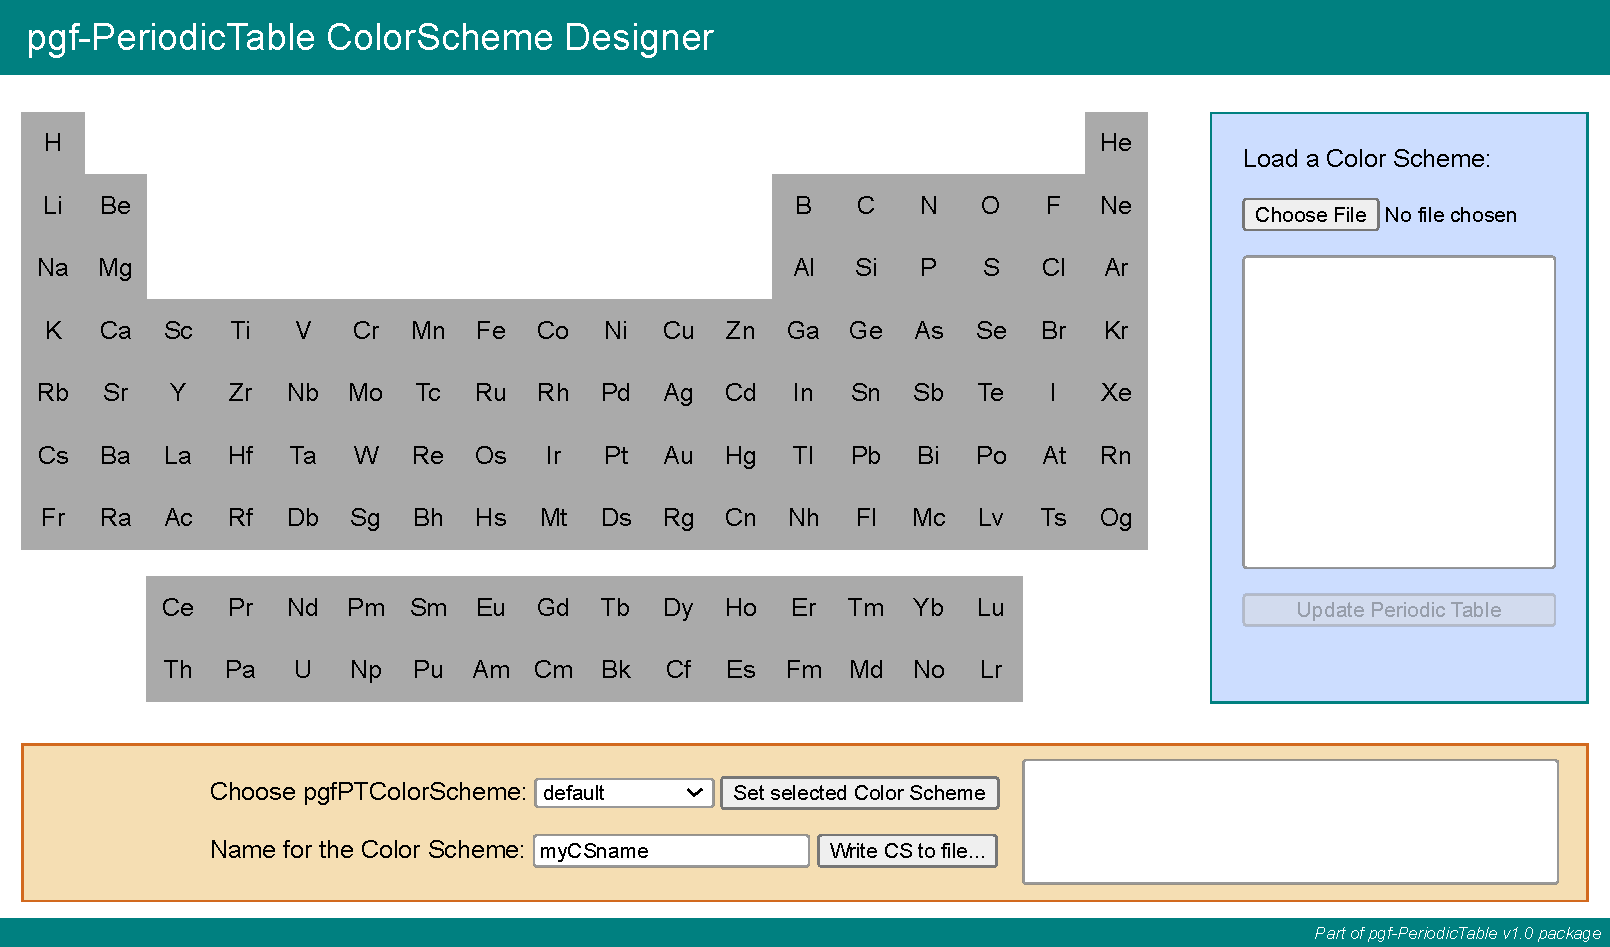
\includegraphics[height=5.2cm]{manualfiles/pgfPTcolorSchemes_html_general.pdf}}
\\ [5pt]\makebox[\linewidth][c]{\href{run:pgfPTcolorSchemes.html}{pgfPTcolorSchemes.html}}
%%%%%%%%%%%%%%%%%%%%%%%%%%%%%%%%%%%%%%%%%%%%%%%%%%%%%%%%%%%%
%\newpage\ \\ [-62pt]
\\ [-32pt]\ %
\def\tmpSection{\bs{pgfPTnewZlist}\lb\red{name}\rb}%
\subsection*{}{\normalfont\large\bfseries\raisebox{1.25pt}{$\mathbf{\blacktriangleright}$}\ Utilization of \tmpSection}%
\index{COMMANDS@\textbf{COMMANDS}!\textbackslash pgfPTnewZlist}%
\label{command:pgfPTnewZlist}\addcontentsline{toc}{subsection}{\texorpdfstring{\tmpSection{}}{\textbackslash pgfPTnewZlist}}%
\\ [4pt]This command makes a user defined atomic numbers' list with the provided \textcolor{red!50!black}{name}. The list can be anything that the {\large\textsf{\textbackslash foreach}} loop, defined in the \txttikz{} package, can understand.
\\ [2pt]{\small For more information on how to use {\normalsize\textsf{\textbackslash foreach}} loop refer to the section \textit{Repeating Things: The Foreach Statement} in the \href{https://www.ctan.org/pkg/pgf}{pgfmanual}}.
\\ [10pt]\pgfPTMnewZlist{myZlist}{1,...,57,72,80,81,...,85}%
\pgfPTnewZlist{myZlist}{1,...,57,72,80,81,...,85}%
\\ [-4pt]\pgfPTMmacrobox{pgfPT}[Z list=myZlist,IUPAC=false]%
\\ [10pt]\makebox[\linewidth][c]{\scalebox{.6}{\pgfPT[Z list=myZlist,IUPAC=false]}}%
\\ [5pt]\pgfPTMline%
\newpage\ \\ [-62pt]
%\\ [-32pt]\ %
\def\tmpSection{\bs{pgfPTsetLanguage}\lb\red{language flag}\rb}%
\subsection*{}{\normalfont\large\bfseries\raisebox{1.25pt}{$\mathbf{\blacktriangleright}$}\ Utilization of \tmpSection}%
\index{COMMANDS@\textbf{COMMANDS}!\textbackslash pgfPTsetLanguage}%
\label{command:pgfPTsetLanguage}\addcontentsline{toc}{subsection}{\texorpdfstring{\tmpSection{}}{\textbackslash pgfPTsetLanguage}}%
\\ [4pt]This command globally changes the default language of the Periodic Table. If a user language has been loaded, the corresponding ISO 639-1 code can also be used as a \red{language flag}.
\\ [10pt]\pgfPTMsetLanguage{pt}%
\pgfPTsetLanguage{pt}%
\\ [-4pt]\pgfPTMmacrobox{pgfPT}[]%
\\ [10pt]\makebox[\linewidth][c]{\scalebox{.6}{\pgfPT[]}}%
\\ [10pt]\pgfPTMsetLanguage{en}%
\pgfPTsetLanguage{en}%
\\ [-4pt]\pgfPTMmacrobox{pgfPT}[]%
\\ [10pt]\makebox[\linewidth][c]{\scalebox{.6}{\pgfPT[]}}%
\\ [5pt]\pgfPTMline%
\newpage
\tikz{\node[text width=\linewidth-8pt,inner xsep=4pt,align=left,fill=black!10,rounded corners=2pt] %
{\small\textcolor{black!50}{\%\ \string\usepackage[userlang=nl]\{pgf-PeriodicTable\}}};}%
\\ [-4pt]\pgfPTMsetLanguage{nl}%
\\ [-4pt]\pgfPTMmacrobox{pgfPT}[]%
\\ [10pt]\makebox[\linewidth][c]{\scalebox{.6}{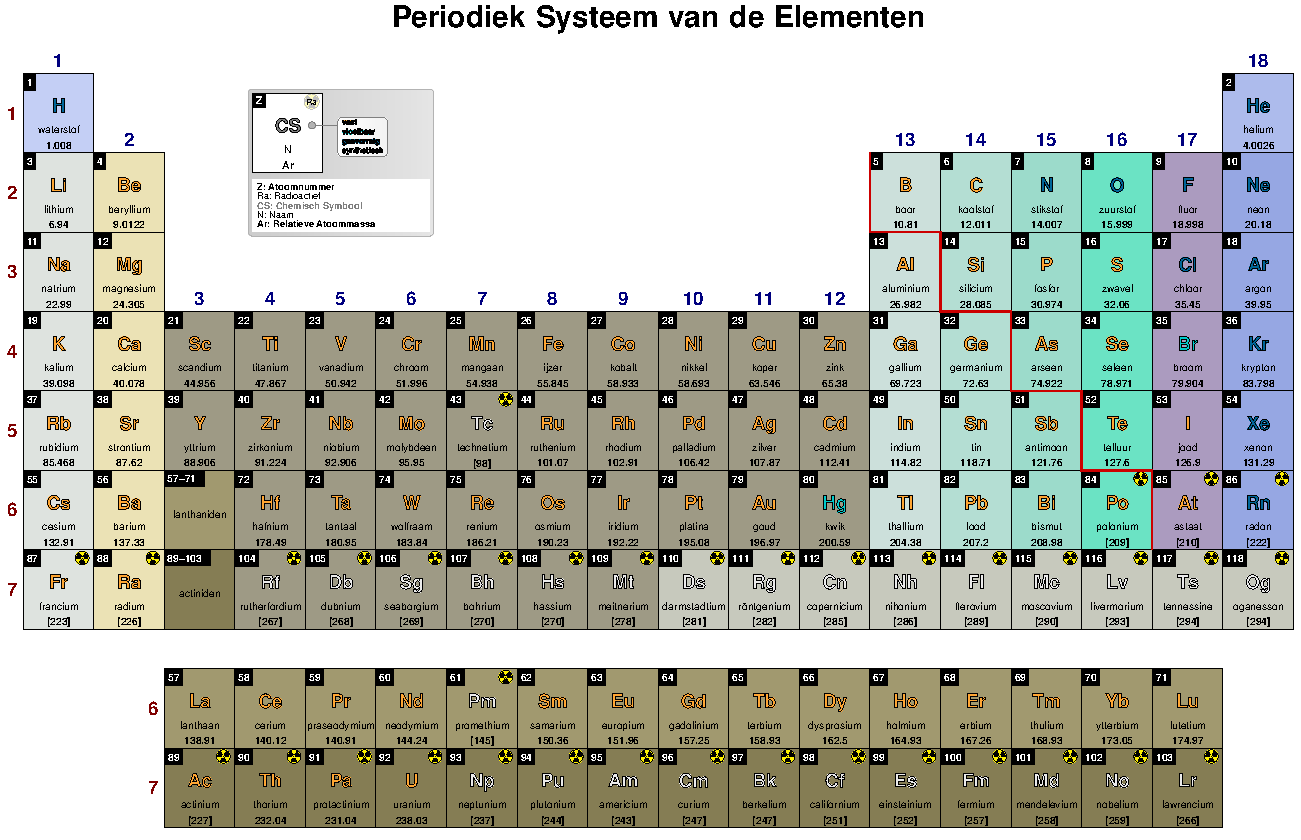
\includegraphics{manualfiles/pgfPT_nl.pdf}}}%
\\ [5pt]\pgfPTMline%
\endinput
%
\newpage%
\def\tmpSection{\bs{pgfPT}}%
\section{\texorpdfstring{Options for \tmpSection: creating a �Periodic Table�}{Options for \textbackslash pgfPT: creating a �Periodic Table�}}
\hypertarget{OPTIONS}{For the commands} \pgfPTMmacro{pgfPT}[] and \pgfPTMmacro{pgfPTstyle}[] there are a set of options available to draw the Periodic Table or any portion of the Periodic Table, as described below.
\\ [6pt]\tikz{\node[text width=\linewidth-6mm,draw=green!70,rounded corners=2pt,fill=black!10!green!10,inner sep=3mm] {%,text justified
\color{green!40!black}The list of options is a comma separated list of any of the following elements:
{\small\begin{itemize}
\item[$\rightsquigarrow$] a \sq{\red{key}} or a \sq{\red{key=value}} pair,
\item[\ding{252}] a \sq{\red{style}} or a \sq{\red{style=value}} pair,
\item[\ding{252}] a \textit{pseudo style} with a proper syntax: \sq{\red{style=\{key 1=value 1, key 2=value 2, \myldots\ , key n=value n\}}}, where none of the \textit{\sq{\red{keys}}} are mandatory.
\end{itemize}}
};}
\\ [3pt]The options \textit{can be divided} in two subsets, one that affects the \textit{appearance} of the \textit{entire} Periodic Table, the other that concerns the \textit{contents} of each cell of the Periodic Table.
\subsection{\texorpdfstring{$\maltese$ Periodic Table options: keys, styles and \itshape pseudo styles}{Periodic Table options}}
The following options and styles are used to \textit{control} the Periodic Table \textit{as a whole} in various aspects, such as the \red{cell width} or \red{cell height}, which elements are displayed (\red{Z list}), whether the title or legend are shown --  \red{show title} or \red{show legend} -- among others.
\label{file:generallayout}%
\subsubsection{\texorpdfstring{\ding{224} General layout}{General layout}}%\vspace{6pt}%
%%%%%%%%%%%%%%%%%%%%%%%%%%%%%%%%%%%%%%%%%%%%%%%%%%%%%%%%%%%%
% Z list
\label{option_Z list}%
\pgfPTMoption[\pgfPTchangedinversion{2.1.5}]{4}{Z list}{all}%
{Set's the list of the elements to display in the Periodic Table. It could be a \lblue{name} or a \lblue{comma sepa\-rated} list of atomic numbers (\hyperlink{Zlistdesc}{see below}), which in turn supports \textit{the dots notation} as explained in the section \textit{Repeating Things: The Foreach Statement} in the \href{https://www.ctan.org/pkg/pgf}{pgfmanual}.\vskip0pt\relax}
\\ [5pt]\pgfPTMmacrobox{pgfPT}[Z list={1,...,36}]%
\\ [5pt]\makebox[\linewidth][c]{\scalebox{.6}{\pgfPT[Z list={1,...,36}]}}%
\\ [5pt]\pgfPTMoptiontxt{%
The possible \lblue{name} is one of the following:
\begin{itembar}
\item\textbf{built-in}:
\begin{itemize}
\item[\raisebox{1pt}{\scriptsize$\vartriangleright\,$}]\sq{all} is equivalent to \green{Z list=\{1,...,118\}}, \ie, all known elements.
\item[\raisebox{1pt}{\scriptsize$\vartriangleright\,$}]\sq{s}, \sq{p}, \sq{d} or \sq{f}, for the elements in the corresponding blocks.
\item[\raisebox{1pt}{\scriptsize$\vartriangleright\,$}]\sq{sp}, \sq{spd}, for the elements resulting from merging the corresponding blocks.
\item[\raisebox{1pt}{\scriptsize$\vartriangleright\,$}]\sq{lanthanoids} or simply \sq{La}, for lanthanoids\red{$\,^\dag$}.
\item[\raisebox{1pt}{\scriptsize$\vartriangleright\,$}]\sq{actinoids} or \sq{Ac}, for actinoids\red{$\,^\dag$}.
\item[\raisebox{1pt}{\scriptsize$\vartriangleright\,$}]\sq{G1*}, \sq{G1}, \myldots\ , \sq{G18}, which are used, respectively, for the elements of \textit{group 1 without hydrogen}, \textit{group 1}, \myldots\ , \textit{group 18}.
\item[\raisebox{1pt}{\scriptsize$\vartriangleright\,$}]\sq{ P1}, \myldots\ , \sq{P7}, \sq{P6*}, \sq{P7*}, which are used, respectively, for the elements of the \textit{1\raisebox{3pt}{\scriptsize st} period}, \myldots\ , \textit{7\raisebox{3pt}{\scriptsize\hspace{.5pt}th} period}, \textit{6\raisebox{3.5pt}{\scriptsize\hspace{.25pt}th} period and lanthanoids}\red{$\,^\dag$}, \textit{7\raisebox{3pt}{\scriptsize\hspace{.5pt}th} period and actinoids}\red{$\,^\dag$}.
\\ [3pt]\makebox[\linewidth][r]{\scriptsize\red{$^\dag\,$}\textit{Depending on the value of the \red{IUPAC} key, the Lanthanum or Actinium are or are not included}.}
\end{itemize}
\item any \textbf{user defined} name via \pgfPTMmacro{pgfPTnewZlist}[]\{name\}\{list\}
\end{itembar}%
}%
\newpage%\vspace{-34pt}\ %
\pgfPTMoptiontxt{%
\hypertarget{Zlistdesc}{Since} \blue{v2.1.5} the \red{Z list} supports a new syntax which makes possible to get \textit{empty} cells \textit{anywhere} in the Periodic Table. The \red{Z list} can be:
\vspace{6pt}
\begin{itembar}
\item a list of numbers -- \green{Z list=\{1,...,118\}} or \green{Z list=\{1,2,3,4,5,6,11,12,13,14,15,16\}}.
\item[]
\item a list of numbers preceded with a star -- \green{Z list=*\{1,...,5,9,10,...,24\}} or \green{Z list=*(\red{options})\{1,...,5,9, 10,...,24\}}.
\begin{itemize}
\item[\raisebox{1pt}{\scriptsize$\vartriangleright\,$}] \red{Z list} preceded only with a star:
\\ It is used to draw the cells skipped in the list without information, but with the atomic number and filling.
\\ [5pt]\pgfPTMmacrobox{pgfPT}[Z list=*{1,...,5,9,10,...,18}]%
\\ [10pt]\makebox[\linewidth][c]{\scalebox{.6}{\pgfPT[Z list=*{1,...,5,9,10,...,18}]}}%
\item[]
\item[\raisebox{1pt}{\scriptsize$\vartriangleright\,$}] \red{Z list} is preceded with a star followed by \red{options}:
\\ It is used to draw the cells skipped in the list without information, with what is shown and how it is shown controlled by the options. There are only two options available -- \red{hide Z} and \red{back color=<color>} -- which can be used separately or as a comma separated pair in any order.
\\ [5pt]\pgfPTMmacrobox{pgfPT}[Z list=*(hide Z){1,...,5,9,10,...,18}]%
\\ [5pt]\makebox[\linewidth][c]{\scalebox{.6}{\pgfPT[Z list=*(hide Z){1,...,5,9,10,...,18}]}}%
\\ [5pt]\pgfPTMmacrobox{pgfPT}[Z list=*({back color=white}){1,...,5,9,10,...,18}]%
\\ [5pt]\makebox[\linewidth][c]{\scalebox{.6}{\pgfPT[Z list=*({back color=white}){1,...,5,9,10,...,18}]}}%
\\ [5pt]\pgfPTMmacrobox{pgfPT}[Z list=*({hide Z,back color=white}){1,...,5,9,10,...,18}]%
\\ [5pt]\makebox[\linewidth][c]{\scalebox{.6}{\pgfPT[Z list=*({hide Z,back color=white}){1,...,5,9,10,...,18}]}}%
\\ [10pt]The \textit{starred} version of the \red{Z list} can be used as an alternative or a complement to the \hyperlink{exMODE}{Exercise layout} mode of the Periodic Table.
\end{itemize}
\end{itembar}%
}%
\\ [-5pt]\pgfPTendoption%
\newpage\vspace{-34pt}\ %
% cell width
\label{option_cell width}%
\pgfPTMoption{4}{cell width}{34pt}%
{Sets the width of each base cell of the Periodic Table.}%
\\ [5pt]\pgfPTMmacrobox{pgfPT}[Z list={1,...,36},cell width=40pt]%
\\ [10pt]\makebox[\linewidth][c]{\scalebox{.6}{\pgfPT[Z list={1,...,36},cell width=40pt]}}%
\\ [5pt]\pgfPTendoption%
% cell height
\label{option_cell height}%
\pgfPTMoption{4}{cell height}{38.25pt}%
{Sets the height of each base cell of the Periodic Table.}%
\\ [5pt]\pgfPTMmacrobox{pgfPT}[Z list={1,...,36},cell height=50pt]%
\\ [10pt]\makebox[\linewidth][c]{\scalebox{.6}{\pgfPT[Z list={1,...,36},cell height=50pt]}}%
\\ [5pt]\pgfPTendoption%
% cell size (style)
\label{style_cell size}%
\pgfPTMstyle{4}{cell size}{38.25pt}%
{Style to set both the width and the height of each base cell of the Periodic Table.}%
\\ [5pt]\pgfPTMmacrobox{pgfPT}[Z list={1,...,36},cell size=40pt]%
\\ [10pt]\makebox[\linewidth][c]{\scalebox{.6}{\pgfPT[Z list={1,...,36},cell size=40pt]}}%
\\ [5pt]\pgfPTendstyle%
\newpage\vspace{-34pt}\ %
% cell line width
\label{option_cell line width}%
\pgfPTMoption{4}{cell line width}{0.4pt}%
{Sets the width of the line surrounding the base cell of the Periodic Table.}%
\\ [5pt]\pgfPTMmacrobox{pgfPT}[Z list={1,...,36},cell line width=2pt]%
\\ [10pt]\makebox[\linewidth][c]{\scalebox{.6}{\pgfPT[Z list={1,...,36},cell line width=2pt]}}%
\\ [5pt]\pgfPTendoption%
% cell line color
\label{option_cell line color}%
\pgfPTMoption{4}{cell line color}{black}%
{Sets the color of the line surrounding the base cell of the Periodic Table.}%
\\ [5pt]\pgfPTMmacrobox{pgfPT}[Z list={1,...,36},cell line color=red]%
\\ [10pt]\makebox[\linewidth][c]{\scalebox{.6}{\pgfPT[Z list={1,...,36},cell line color=red]}}%
\\ [5pt]\pgfPTendoption%
% cell style
\label{option_cell style}%
\pgfPTMoption{4}{cell style}{\{\}}%
{Loads a named cell style, built via \pgfPTMmacro{pgfPTbuildcellstyle}[], to use as a layout for each cell of the Periodic Table.}%
\\ [5pt]\pgfPTMbuildcellstyle{myname}(5,3)[(1;1-2;Z),(1;3;ls),(2-3;1.5-2.5;CS),(4;1-3;name),(5;1-3;eConfignl)]%
\pgfPTbuildcellstyle{myname}(5,3)[(1;1-2;Z),(1;3;ls),(2-3;1.5-2.5;CS),(4;1-3;name),(5;1-3;eConfignl)]%
\\ [-4pt]\pgfPTMmacrobox{pgfPT}[Z list={1,...,36},cell style=myname]%
\\ [10pt]\makebox[\linewidth][c]{\scalebox{.6}{\pgfPT[Z list={1,...,36},cell style=myname]}}%
\\ [5pt]\pgfPTendoption%
% cell={w=??,h=??,s=??,lw=??,lc=??,style=??} (pseudo style)
\newpage\vspace{-34pt}\ %
\label{style_cell}%
\pgfPTMstyle{4}{cell}{\{w=34pt,h=38.25pt,lw=.4pt,lc=black\}}%
{\textit{Pseudo style} to set the cell \textbf{w}idth, the cell \textbf{h}eight, the cell \textbf{s}ize, the cell \textbf{l}ine \textbf{w}idth, the cell \textbf{l}ine \textbf{c}olor and/or the cell \textbf{style}. None of the \textit{keys} -- w, h, s, lw, lc and style -- are mandatory.
\\ [3pt]\makebox[\linewidth][c]{\use{cell=\{w=<length>,h=<length>,s=<length>,lw=<length>,lc=<color>,style=<name>\}}}%
}%
\\ [5pt]\pgfPTMmacrobox{pgfPT}[Z list={1,...,36},cell={w=40pt,h=50pt,lw=.6pt,lc=blue}]%
\\ [10pt]\makebox[\linewidth][c]{\scalebox{.6}{\pgfPT[Z list={1,...,36},cell={w=40pt,h=50pt,lw=.6pt,lc=blue}]}}%
\\ [5pt]\pgfPTendstyle%
% font
\vfill%
\label{option_font}%
\pgfPTMoption[\pgfPTchangedinversion{2.1.5}]{4}{font}{\raisebox{-\baselineskip}{%
\vbox{\hsize=.675\linewidth\hbox{phv (\textrm{pdf\LaTeX}); TeX Gyre Heros (\textrm{Xe\LaTeX} or \textrm{Lua\LaTeX});}%
\hbox{BabelStone Han (for Chinese)}}}%
}%
%phv (\textrm{pdf\LaTeX}); TeX Gyre Heros (\textrm{Xe\LaTeX} or \textrm{Lua\LaTeX});\par BabelStone Han (for Chinese)}%
{\ \\ [8pt]Sets the font family, via the proper \textrm{\LaTeX} \textit{font name}, to use in the Periodic Table.
\\ [2pt]When \textrm{pdf\LaTeX} is used to typeset the Periodic Table the \textit{default} font is \textit{phv}, \ie, the Helvetica font. In this case the value of the \red{font} key can be any \textrm{\LaTeX} \textit{font name} known to the local \textrm{\LaTeX} installation.
\\ [2pt]When \textrm{Xe\LaTeX} or \textrm{Lua\LaTeX} are used to typeset the Periodic Table the \textit{default} font is \textit{TeX Gyre Heros}, a closest alternative to Helvetica font. In this case the value of the \red{font} key can be any \textit{font name known to your Operating System or} \textrm{\LaTeX} \textit{distribuition} and with \textrm{Lua\LaTeX} it can also be any \textit{font name available in your} \textrm{TEXMF} \textit{tree}.
\\ [2pt]If the Chinese language is loaded the default font is BabelStone Han. See \hyperlink{subsec::zhLang}{Chinese} user language for more details.
\\ \hfill\scriptsize See \textit{\textrm{\LaTeX} font names} below or the \href{https://ftp.eq.uc.pt/software/TeX/macros/unicodetex/latex/fontspec/fontspec.pdf\#page=9}{fontspec documentation} for further details.\normalsize\\ \ }%
\\ [10pt]Examples with \textrm{pdf\LaTeX}:
\\ [5pt]\pgfPTMmacrobox{pgfPT}[Z list={1,...,36},font=ptm]%
\\ [10pt]\makebox[\linewidth][c]{\scalebox{.6}{\pgfPT[Z list={1,...,36},font=ptm]}}%
\newpage%
\pgfPTMmacrobox{pgfPT}[Z list={1,...,36},font=RobotoSlab-TLF]%
\\ [10pt]\makebox[\linewidth][c]{\scalebox{.6}{\pgfPT[Z list={1,...,36},font=RobotoSlab-TLF]}}%
\\ [10pt]\pgfPTMoptiontxt{%
\textit{\textrm{\LaTeX} font names}:
\begin{itembar}
\item The \textrm{\LaTeX} font names commonly available in \textrm{\LaTeX} distributions are:
\\ [5pt]\begin{minipage}[t]{.5\linewidth}
-- \textbf{\fontfamily{cmr}\selectfont Serif fonts}
\begin{itemize}
\item[\raisebox{1pt}{\scriptsize$\vartriangleright\,$}] \fnt{cmr}{Computer Modern Roman}
\item[\raisebox{1pt}{\scriptsize$\vartriangleright\,$}] \fnt{lmr}{Latin Modern Roman}
\item[\raisebox{1pt}{\scriptsize$\vartriangleright\,$}] \fnt{pbk}{Bookman}
\item[\raisebox{1pt}{\scriptsize$\vartriangleright\,$}] \fnt{bch}{Charter}
\item[\raisebox{1pt}{\scriptsize$\vartriangleright\,$}] \fnt{pnc}{New Century Schoolbook}
\item[\raisebox{1pt}{\scriptsize$\vartriangleright\,$}] \fnt{ppl}{Palatino}
\item[\raisebox{1pt}{\scriptsize$\vartriangleright\,$}] \fnt{ptm}{Times}
\end{itemize}
\end{minipage}%
\begin{minipage}[t]{.5\linewidth}
-- \textbf{\small\textsf{Sans Serif fonts}}
\begin{itemize}
\item[\raisebox{1pt}{\scriptsize$\vartriangleright\,$}] \fnt{cmss}{Computer Modern Sans Serif}
\item[\raisebox{1pt}{\scriptsize$\vartriangleright\,$}] \fnt{lmss}{Latin Modern Sans Serif}
\item[\raisebox{1pt}{\scriptsize$\vartriangleright\,$}] \fnt{pag}{Avant Garde}
\item[\raisebox{1pt}{\scriptsize$\vartriangleright\,$}] \fnt{phv}{Helvetica}
\end{itemize}
\end{minipage}
\\ \ %
\item There are other fonts available to \textrm{\LaTeX} that require installation of the corresponding packages:
\begin{itemize}
\item[\raisebox{1pt}{\scriptsize$\vartriangleright\,$}] the \href{https://ctan.org/pkg/roboto}{roboto package} provides the following fonts:
\\ \textbullet\ \fnt{Roboto-TLF}{Roboto tabular lining}
\\ \textbullet\ \fnt{Roboto-LF}{Roboto proportional lining}
\\ \textbullet\ \fnt{Roboto-OsF}{Roboto proportional oldstyle}
\\ \textbullet\ \fnt{Roboto-TOsF}{Roboto tabular oldstyle}
\\ \textbullet\ \fnt{RobotoSlab-TLF}{RobotoSlab proportional lining}
\\ \textbullet\ \fnt{RobotoSlab-OsF}{RobotoSlab proportional oldstyle}
\\ \textbullet\ \fnt{RobotoSlab-TOsF}{RobotoSlab tabular oldstyle}
\\ \textbullet\ \fnt{RobotoMono-TLF}{RobotoMono proportional lining}
\item[\raisebox{1pt}{\scriptsize$\vartriangleright\,$}] the \href{https://ctan.org/pkg/frcursive}{frcursive package} provides the \fnt{frc}{French Cursive} font.
\item[\raisebox{1pt}{\scriptsize$\vartriangleright\,$}] the \href{https://ctan.org/pkg/miama}{miama package} provides the \fnt{fmm}{Miama Nueva} font.
\item[\raisebox{1pt}{\scriptsize$\vartriangleright\,$}] \myldots
\end{itemize}
\end{itembar}%
\vspace{10pt}
\makebox[\linewidth][c]{For more information about fonts visit the \href{https://tug.org/FontCatalogue/}{TUG Font Catalogue}}
\\ \ %
}%
\\ [10pt]Examples with \textrm{Xe\LaTeX} or \textrm{Lua\LaTeX}:
\\ [5pt]\pgfPTMmacrobox{pgfPT}[Z list={1,...,36},font=Verdana,CS font=\string\fontspec{Mistral}\string\selectfont]%
\\ [10pt]\makebox[\linewidth][c]{\scalebox{.6}{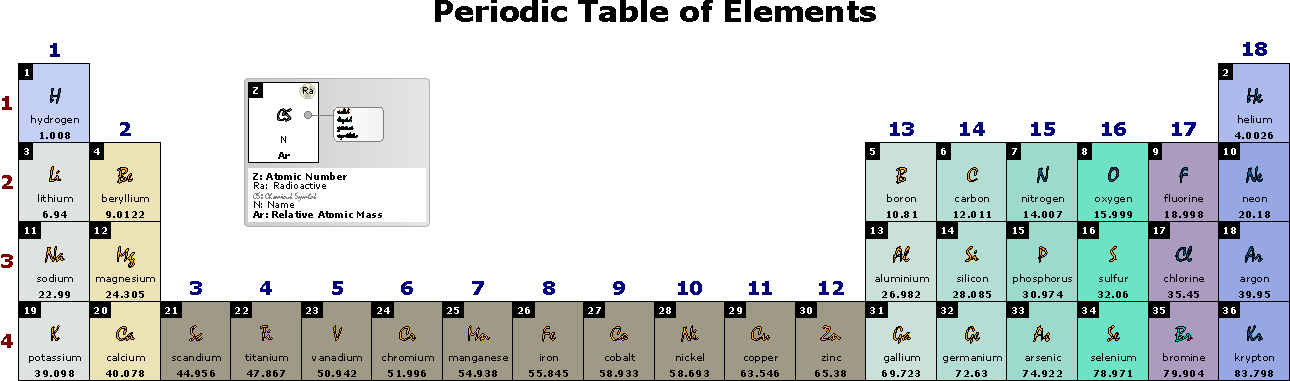
\includegraphics{manualfiles/pgfPTfontLuaXeLaTeX1.pdf}}}%
\newpage
\pgfPTMmacrobox{pgfPT}[Z list={1,...,36},font=Arial,CS font=\string\fontspec{LCALLIG.TTF}\string\selectfont]%
\\ [10pt]\makebox[\linewidth][c]{\scalebox{.6}{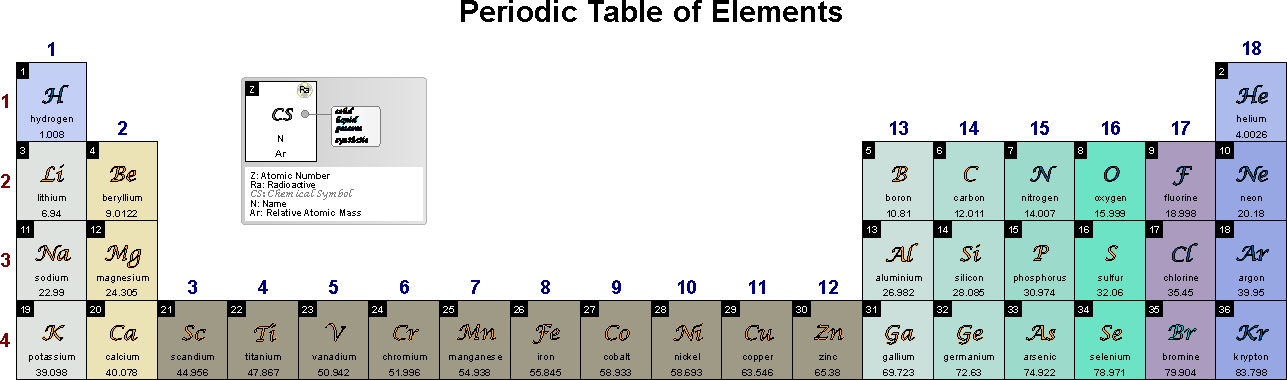
\includegraphics{manualfiles/pgfPTfontLuaXeLaTeX2.pdf}}}%
\\ [5pt]\pgfPTendoption%
\vfill
% back color
\label{option_back color}%
\pgfPTMoption{4}{back color}{white}%
{Sets the background of each cell of the Periodic Table. It only takes effect if the \red{back color scheme} key is set to \red{solid}}%
\\ [5pt]\pgfPTMmacrobox{pgfPT}[Z list={1,...,36},back color=black!15]%
\\ [10pt]\makebox[\linewidth][c]{\scalebox{.6}{\pgfPT[Z list={1,...,36},back color=black!15]}}%
\\ [10pt]\pgfPTMmacrobox{pgfPT}[Z list={1,...,36},back color scheme=solid,back color=black!15]%
\\ [10pt]\makebox[\linewidth][c]{\scalebox{.6}{\pgfPT[Z list={1,...,36},back color scheme=solid,back color=black!15]}}%
\\ [5pt]\pgfPTendoption%
\newpage\vspace{-34pt}\ %
% back color scheme
\label{option_back color scheme}%
\pgfPTMoption{4}{back color scheme}{pgfPTdefault}%
{Sets a \blue{named} back color scheme for the Periodic Table.}%
\\ [2.5pt]\pgfPTMmacrobox{pgfPT}[back color scheme=pgfPTSoft]%
\\ [2.5pt]\makebox[\linewidth][c]{\scalebox{.6}{\pgfPT[back color scheme=pgfPTSoft]}}%
\vfill
\pgfPTMoptiontxt{%
The possible \lblue{name} is one of the following:
\begin{itembar}
\item\textbf{built-in}:
\begin{itemize}
\item[\raisebox{1pt}{\scriptsize$\vartriangleright\,$}]\sq{pgfPTSoft}, a soft color scheme that distinguishes metals, non metals, silicon and germanium, lanthanoids and actinoids.
\item[\raisebox{1pt}{\scriptsize$\vartriangleright\,$}]\sq{pgfPTJmol}, is the color scheme used in the computer software \href{http://jmol.sourceforge.net/}{Jmol}: an open-source Java viewer for chemical structures in 3D.
\item[\raisebox{1pt}{\scriptsize$\vartriangleright\,$}]\sq{pgfPTCPK}, is the color scheme of the popular color convention for distinguishing atoms of different chemical
elements in molecular models. The scheme is named after the CPK molecular models designed by chemists Robert Corey and Linus Pauling, and improved by Walter Koltun.
\item[\raisebox{1pt}{\scriptsize$\vartriangleright\,$}]\sq{pgfPTRasmol}, is the color scheme used in the computer software \href{http://www.rasmol.org/}{RasMol}, a program for molecular graphics visualization originally developed by Roger Sayle.
\item[\raisebox{1pt}{\scriptsize$\vartriangleright\,$}]\sq{pgfPTRasmolNew}, is a color scheme used in RasMol with revision of CPK colors made by C. Chigbo (RasMol 2.7.3).
\item[\raisebox{1pt}{\scriptsize$\vartriangleright\,$}]\sq{pgfPTWikipediaII}, is the color scheme based on the most recent (\href{https://commons.wikimedia.org/wiki/File:Simple_Periodic_Table_Chart-en.svg\#filehistory}{November 2020 to present}) \href{https://en.wikipedia.org/wiki/Periodic_table\#Classification_of_elements}{Wikipedia Periodic Table of Elements}.
\item[\raisebox{1pt}{\scriptsize$\vartriangleright\,$}]\sq{pgfPTWikipediaI}, is the color scheme based on the previous (\href{https://commons.wikimedia.org/wiki/File:Simple_Periodic_Table_Chart-en.svg\#filehistory}{until October 2020}) Wikipedia Periodic Table of Elements.
    \\ [2pt]\tikz{\node[text width=\linewidth-3mm,draw=green!70,rounded corners=2pt,fill=black!10!green!10,inner sep=1.5mm] {%
    The higher the number on Wikipedia, the more recent the color scheme.
    \\ For backwards compatibility (and also for simplicity) pgfPTWikipedia points to pgfPTWikipediaII.% and csWikipedia points to csWikipediaII,
    };}
\item[\raisebox{1pt}{\scriptsize$\vartriangleright\,$}]\sq{pgfPTMNM}, is designed to show \textbf{M}etals and \textbf{N}on \textbf{M}etals in two different colors, showing also the semi-metals in a third color.
\item[\raisebox{1pt}{\scriptsize$\vartriangleright\,$}]\sq{pgfPTPS}, is designed to show the \textbf{P}hysical \textbf{S}tate of the elements at normal temperature and pressure (NTP) in different colors.
\item[\raisebox{1pt}{\scriptsize$\vartriangleright\,$}]\sq{pgfPTRadio}, is designed to show the \textbf{R}adioactive elements in one color and the non radioactive elements in another color.
\item[\raisebox{1pt}{\scriptsize$\vartriangleright\,$}]\sq{pgfPTBlocks}, for showing the elements in each block of the Periodic Table with the same color.
\item[\raisebox{1pt}{\scriptsize$\vartriangleright\,$}]\sq{solid}, to show the background of each cell of the Periodic Table with the same color specified by the key \sq{\red{back color}}.
\end{itemize}
\item any \textbf{user defined} name via \bs{pgfPTnewColorScheme}\lb\red{name}\rb\lb\red{color list}\rb%
\end{itembar}%
}%
\\ [-7.5pt]\pgfPTendoption%
\newpage\ \vfill%
\textit{It is possible to set the \red{back color scheme} key with the built-in names using the following styles}:\vfill%
% STYLES for back color schemes -> csSoft,csJmol,csCPK,csRasmol,csRasmolNew,csWikipedia,csMNM,csPS,csRadio,csBlocks,csSolid
\label{style_CSchemes}%
\pgfPTMstyle{4}{csSolid}{white}%
{A style equivalent to \red{back color scheme=solid,back color=\#1}}%
\\ [5pt]\pgfPTMmacrobox{pgfPT}[csSolid]%
\\ [10pt]\makebox[\linewidth][c]{\scalebox{.6}{\pgfPT[csSolid]}}%
\\ [10pt]\pgfPTMmacrobox{pgfPT}[csSolid=black!15]%
\\ [10pt]\makebox[\linewidth][c]{\scalebox{.6}{\pgfPT[csSolid=black!15]}}%
\\ [5pt]\pgfPTendstyle%
\newpage\vspace{-34pt}\ %
%\foreach \csName/\x in {Soft/0,Jmol/1,CPK/0,Rasmol/1,RasmolNew/0,Wikipedia/1,MNM/0,PS/1,Radio/0,Blocks/1}{%
\foreach \csName/\x\desc in {Soft/0/Soft,Jmol/1/Jmol,CPK/0/CPK,Rasmol/1/Rasmol,RasmolNew/0/RasmolNew,%
Wikipedia/1/WikipediaII,WikipediaI/0/WikipediaI,WikipediaII/1/WikipediaII,MNM/0/MNM,PS/1/PS,Radio/0/Radio,Blocks/1/Blocks}{%
\pgfPTMstyletxt{4}{cs\csName}{no value}%
{A style equivalent to \red{back color scheme=pgfPT\desc}}%
\\ [5pt]\pgfPTMmacrobox{pgfPT}[cs\csName]%
\\ [10pt]\makebox[\linewidth][c]{\scalebox{.6}{\pgfPT[cs\csName]}}%
\\ [0pt]\pgfPTendstyle%
\ifnum\x=1\relax%
\newpage\vspace{-34pt}\ %
\fi%
}%
% paper (style)
\label{style_paper}%
\pgfPTMstyle{4}{background}{\{\}}%
{A style to set the background of the Periodic Table, built with any of the \txttikz\ keys that can be applied to a path construction.}%
\\ [5pt]\pgfPTMmacrobox{pgfPT}[background={draw=red,line width=2pt,fill=red!10}]%
\\ [10pt]\makebox[\linewidth][c]{\scalebox{.6}{\pgfPT[background={draw=red,line width=2pt,fill=red!10}]}}%
\\ [10pt]\tikz{\node[text width=\linewidth-8pt,inner xsep=4pt,fill=black!10,rounded corners=2pt,font=\small] {\textcolor{black!70}{\textbackslash usetikzlibrary\{shadows\}}};}
\\ [-4pt]\pgfPTMmacrobox{pgfPT}[background={left color=red!10,right color=green!10,postaction={drop shadow={left color=red!10,right color=green!10}}}]%
\\ [10pt]\makebox[\linewidth][c]{\scalebox{.6}{\pgfPT[background={left color=red!10,right color=green!10,postaction={drop shadow={left color=red!10,right color=green!10}}}]}}%
\\ [5pt]\pgfPTendstyle%
% IUPAC
\label{option_IUPAC}%
\pgfPTMoption{4}{IUPAC}{true}%
{When set to true draws the periodic table with \textit{lanthanum} and \textit{actinium} appended to block f and the labels \textit{lanthanoids} and \textit{actinoids} are placed at group 3, substituting \textit{lanthanum} and \textit{actinium}. When \red{IUPAC} is set to false, \textit{lanthanum} and \textit{actinium} are shown in group 3 and the labels \textit{lanthanoids} and \textit{actinoids} are place near the \textit{f block} (if the key \red{show label LaAc} is set to true).
}%
\\ [5pt]\pgfPTMmacrobox{pgfPT}[]%
\\ [10pt]\makebox[\linewidth][c]{\scalebox{.6}{\pgfPT}}%
\\ [10pt]\pgfPTMmacrobox{pgfPT}[IUPAC=false]%
\\ [10pt]\makebox[\linewidth][c]{\scalebox{.6}{\pgfPT[IUPAC=false]}}%
\\ [5pt]\pgfPTendoption%
\newpage\vspace{-34pt}\ %
% show label LaAc
\label{option_show label LaAc}%
\pgfPTMoption{4}{show label LaAc}{\{\}}%
{Determines when the labels \sq{lanthanoids} and \sq{actinoids} are shown (\red{true}) or not shown (\red{false}) near the f block. When the \red{IUPAC} key is set to true, the default behavior is to show the labels and when the \red{IUPAC} key is set to false, the default behavior is to hide the labels. This \textit{default behavior} \textbf{can be overridden by this key} setting it to true, to show the labels, or to false to hide them, independently of the value of the \red{IUPAC} key.
}%
\\ [5pt]\pgfPTMnewZlist{myZlist}{55,...,118}%
\pgfPTnewZlist{myZlist}{55,...,118}%
\\ [-4pt]\pgfPTMmacrobox{pgfPTstyle}[show title=false,show legend=false,show group numbers=false]%
\pgfPTstyle[show title=false,show legend=false,show group numbers=false]%
\\ [-4pt]\pgfPTMmacrobox{pgfPT}[Z list=myZlist]%
\\ [5pt]\makebox[\linewidth][c]{\scalebox{.6}{\pgfPT[Z list=myZlist]}}%
\\ [5pt]\pgfPTMmacrobox{pgfPT}[Z list=myZlist,show label LaAc=true]%
\\ [5pt]\makebox[\linewidth][c]{\scalebox{.6}{\pgfPT[Z list=myZlist,show label LaAc=true]}}%
\\ [5pt]\pgfPTMmacrobox{pgfPT}[Z list=myZlist,IUPAC=false]%
\\ [5pt]\makebox[\linewidth][c]{\scalebox{.6}{\pgfPT[Z list=myZlist,IUPAC=false]}}%
\\ [5pt]\pgfPTMmacrobox{pgfPT}[Z list=myZlist,IUPAC=false,show label LaAc=false]%
\\ [5pt]\makebox[\linewidth][c]{\scalebox{.6}{\pgfPT[Z list=myZlist,IUPAC=false,show label LaAc=false]}}%
\\ [5pt]\pgfPTendoption%
\newpage\vspace{-34pt}\ %
% label LaAc font
\label{option_label LaAc font}%
\pgfPTMoption{4}{label LaAc font}{\string\footnotesize\string\itshape}%
{Sets the font for the labels \sq{lanthanoids} and \sq{actinoids}.}%
\\ [5pt]\pgfPTMmacrobox{pgfPT}[label LaAc font=\string\bfseries,Z list=myZlist,IUPAC=false]%
\\ [10pt]\makebox[\linewidth][c]{\scalebox{.6}{\pgfPT[label LaAc font=\bfseries,Z list=myZlist,IUPAC=false]}}%
\\ [5pt]\pgfPTMmacrobox[l]{pgfPTresetstyle}[]%
\pgfPTresetstyle%
\\ [-10pt]\pgfPTendoption%
% languages
\vfill
\label{option_languages}%
\pgfPTMoption[\pgfPTchangedinversion{2.1.0}]{4}{languages}{\{\}}%
{Sets a language list to use in the Periodic Table. It is a comma separated list of language flags: \sq{pt}, \sq{en}, \sq{fr}, \sq{de}, \sq{it}, \sq{es} or \sq{br}. If a user language has been loaded, the corresponding ISO 639-1 code can also be used as a language flag. \textit{This key locally overrides the default language, that is, the language loaded at package inclusion}.\\ \ }%
\\ [5pt]\pgfPTMmacrobox{pgfPT}[Z list={1,...,36},languages=pt]%
\\ [10pt]\makebox[\linewidth][c]{\scalebox{.6}{\pgfPT[Z list={1,...,36},languages=pt]}}%
\\ [10pt]\pgfPTMmacrobox{pgfPT}[Z list={1,...,36},cell style=pgfPT2lang,languages={en,fr}]%
\\ [10pt]\makebox[\linewidth][c]{\scalebox{.6}{\pgfPT[Z list={1,...,36},cell style=pgfPT2lang,languages={en,fr}]}}%
\newpage%\\ [10pt]
\tikz{\node[text width=\linewidth-8pt,inner xsep=4pt,align=left,fill=black!10,rounded corners=2pt] %
{\small\textcolor{black!50}{\%\ \string\usepackage[userlang=nl]\{pgf-PeriodicTable\}}};}%
\\ [-4pt]\pgfPTMmacrobox{pgfPT}[Z list={1,...,36},cell style=pgfPT2lang,languages={nl,en}]%
\\ [10pt]\makebox[\linewidth][c]{\scalebox{.6}{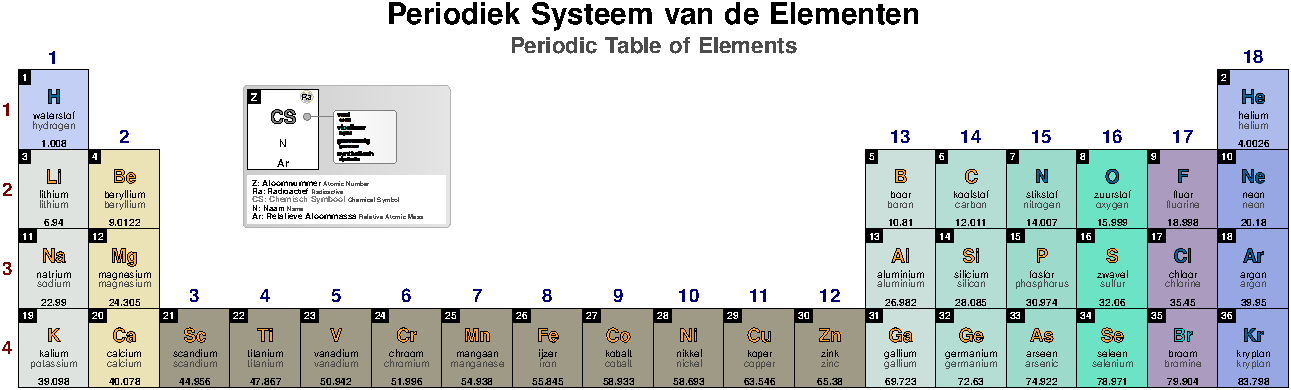
\includegraphics{manualfiles/pgfPT_nl_en.pdf}}}%
\\ [10pt]\pgfPTMmacrobox{pgfPT}[Z list={1,...,36},cell style=pgfPT3lang,languages={pt,fr,it}]%
\\ [10pt]\makebox[\linewidth][c]{\scalebox{.6}{\pgfPT[Z list={1,...,36},cell style=pgfPT3lang,languages={pt,fr,it}]}}%
\\ [10pt]\pgfPTMoptiontxt{%
When using a set of languages, space to accommodate the names in each cell must be provided by building a suitable cell - typically one cell row per language. The cell styles used in the two examples above are built-in and serve this purpose.
\vspace{2.5pt}%
\begin{itembar}
\item\pgfPTpreviewcellstyle[1.5]{pgfPT2lang}\vspace{-10pt}\item\pgfPTpreviewcellstyle[1.5]{pgfPT3lang}
\end{itembar}
\vspace{2.5pt}%
Also, the space for the title should be taken into account -- if using more then three languages, the legend must be \textit{turned off}, otherwise the title overlaps the legend.
}%
\\ [-10pt]\pgfPTendoption%
%\newpage%\vfill%
% other languages font
\label{option_other languages font}%
\pgfPTMoption{4}{other languages font}{\string\tiny}%
{Sets the font used in \textit{other languages}, \ie, the languages started at the second entry of the list provide to the \red{languages} key.}%
\newpage\enlargethispage{\baselineskip}%\\ [5pt]
\pgfPTMmacrobox{pgfPT}[Z list={1,...,36},cell style=pgfPT3lang,languages={en,es,br}, other languages font=\string\tiny\string\bfseries]%
\\ [10pt]\makebox[\linewidth][c]{\scalebox{.6}{\pgfPT[Z list={1,...,36},cell style=pgfPT3lang,languages={en,es,br},other languages font=\tiny\bfseries]}}%
\\ [0pt]\pgfPTendoption%
% other languages color
\label{option_other languages color}%
\pgfPTMoption{4}{other languages color}{black!70}%
{Sets the color of the font used in \textit{other languages}.}%
\\ [5pt]\pgfPTMmacrobox{pgfPT}[Z list={1,...,36},cell style=pgfPT3lang,languages={en,pt,br}, other languages color=purple]%
\\ [10pt]\makebox[\linewidth][c]{\scalebox{.6}{\pgfPT[Z list={1,...,36},cell style=pgfPT3lang,languages={en,pt,br}, other languages color=purple]}}%
\\ [0pt]\pgfPTendoption%
% other lang={f=??,c=??}
\label{style_other lang}%
\pgfPTMstyle{4}{other lang}{\{f=\string\tiny,c=black!70\}}%
{\textit{Pseudo style} to set the keys: other languages \textbf{f}ont and/or other languages \textbf{c}olor. %
None of the \textit{keys} -- f and c -- are mandatory.
\\ [3pt]\makebox[\linewidth][c]{\use{other lang=\{f=<font commands>,c=<color>\}}}%
}%
\\ [5pt]\pgfPTMmacrobox{pgfPT}[Z list={1,...,36},cell style=pgfPT3lang,languages={en,fr,de}, other lang={f=\string\tiny\string\itshape,c=blue}]%
\\ [10pt]\makebox[\linewidth][c]{\scalebox{.6}{\pgfPT[Z list={1,...,36},cell style=pgfPT3lang,languages={en,fr,de}, other lang={f=\tiny\itshape,c=blue}]}}%
\\ [0pt]\pgfPTendstyle%
% show MNM line
\label{option_show MNM line}%
\pgfPTMoption{4}{show MNM line}{true}%
{If set to \red{true} a line separating metals from non metals is shown in the Periodic Table. The line starts at the upper left corner of the cell of boron (2\raisebox{3.5pt}{\footnotesize nd} period, group 13) and ends at the lower right corner of polonium (6\raisebox{3.5pt}{\footnotesize th} period, group 16). If set to \red{false} no line is drawn.
}%
\\ [5pt]\pgfPTMmacrobox{pgfPT}[Z list=spd]%
\\ [10pt]\makebox[\linewidth][c]{\scalebox{.6}{\pgfPT[Z list=spd]}}%
\\ [10pt]\pgfPTMmacrobox{pgfPT}[show MNM line=false]%Z list=spd,
\\ [10pt]\makebox[\linewidth][c]{\scalebox{.6}{\pgfPT[show MNM line=false]}}%Z list=spd,
\\ [10pt]\pgfPTMmacrobox{pgfPT}[Z list={1,...,36}]%
\\ [10pt]\makebox[\linewidth][c]{\scalebox{.6}{\pgfPT[Z list={1,...,36}]}}%Z list=spd,
\\ [0pt]\pgfPTendoption%
%\newpage\vspace{-34pt}\ %
% MNM line color
\label{option_MNM line color}%
\pgfPTMoption{4}{MNM line color}{red!80!black}%
{Sets the color of the \textit{MNM line}.}%
\\ [5pt]\pgfPTMmacrobox{pgfPT}[MNM line color=green]%Z list=spd,
\\ [10pt]\makebox[\linewidth][c]{\scalebox{.6}{\pgfPT[MNM line color=green]}}%Z list=spd,
\\ [0pt]\pgfPTendoption%
% MNM line width
\label{option_MNM line width}%
\pgfPTMoption{4}{MNM line width}{.8pt}%
{Sets the width of the \textit{MNM line}.}%
\\ [5pt]\pgfPTMmacrobox{pgfPT}[MNM line width=1.5pt]%Z list=spd,
\\ [10pt]\makebox[\linewidth][c]{\scalebox{.6}{\pgfPT[MNM line width=1.5pt]}}%Z list=spd,
\\ [0pt]\pgfPTendoption%
% MNM={c=??,w=??} (pseudo style)
\label{style_MNM}%
\pgfPTMstyle{4}{MNM}{\{c=red!80!black,w=.8pt\}}%
{\textit{Pseudo style} to set the \textit{MNM line} \textbf{c}olor and/or \textbf{w}idth. None of the \textit{keys} -- c and w -- are mandatory. The key \red{show MNM line} is set to \red{true}.
\\ [3pt]\makebox[\linewidth][c]{\use{MNM=\{c=<color>,w=<length>\}}}%
}%
\\ [5pt]\pgfPTMmacrobox{pgfPT}[MNM={w=1.5pt,c=red}]%Z list=spd,
\\ [10pt]\makebox[\linewidth][c]{\scalebox{.6}{\pgfPT[MNM={w=1.5pt,c=red}]}}%Z list=spd,
\\ [0pt]\pgfPTendstyle%
\endinput%
%
\label{file:TitleLegend}%
\vfill%
\subsubsection{\texorpdfstring{\ding{224} Title and Legend}{Title and Legend}}\vspace{6pt}
%%%%%%%%%%%%%%%%%%%%%%%%%%%%%%%%%%%%%%%%%%%%%%%%%%%%%%%%%%%%
% show title
\label{option_show title}%
\pgfPTMoption{4}{show title}{true}%
{When set to \red{true} the title is shown, otherwise the title (Periodic Table of elements) is not shown.}%
\\ [5pt]\pgfPTMmacrobox{pgfPT}[Z list={1,...,36}]%
\\ [10pt]\makebox[\linewidth][c]{\scalebox{.6}{\pgfPT[Z list={1,...,36}]}}%
\newpage%\\ [10pt]
\pgfPTMmacrobox{pgfPT}[Z list={1,...,36},show title=false]%
\\ [10pt]\makebox[\linewidth][c]{\scalebox{.6}{\pgfPT[Z list={1,...,36},show title=false]}}%
\\ [0pt]\pgfPTendoption%
% title font
\label{option_title font}%
\pgfPTMoption{4}{title font}{\string\Large\string\bfseries}%
{Sets the font used in the title.}%
\\ [5pt]\pgfPTMmacrobox{pgfPT}[Z list={1,...,36},title font=\string\Huge\string\itshape]%
\\ [10pt]\makebox[\linewidth][c]{\scalebox{.6}{\pgfPT[Z list={1,...,36},title font=\Huge\itshape]}}%
\\ [0pt]\pgfPTendoption%
% title color
\label{option_title color}%
\pgfPTMoption{4}{title color}{black}%
{Sets the title color.}%
\\ [5pt]\pgfPTMmacrobox{pgfPT}[Z list={1,...,36},title color=green!50!black]%
\\ [10pt]\makebox[\linewidth][c]{\scalebox{.6}{\pgfPT[Z list={1,...,36},title color=green!50!black]}}%
\\ [0pt]\pgfPTendoption%
\vfill%
% title (pseudo style)
\label{style_title}%
\pgfPTMstyle{4}{title}{\{f=\string\Large\string\bfseries,c=black\}}%
{\textit{Pseudo style} to set the keys: title \textbf{f}ont and/or title \textbf{c}olor. None of the \textit{keys} -- f and c -- are mandatory.
The key \red{show title} is set to \red{true}.
\\ [3pt]\makebox[\linewidth][c]{\use{title=\{f=<font commands>,c=<color>\}}}%
}%
\vfill%
\newpage%\\ [5pt]
\pgfPTMmacrobox{pgfPT}[Z list={1,...,36},title={f=\string\Huge,c=teal}]%
\\ [10pt]\makebox[\linewidth][c]{\scalebox{.6}{\pgfPT[Z list={1,...,36},title={f=\Huge,c=teal}]}}%
\\ [0pt]\pgfPTendstyle%
% show legend
\label{option_show legend}%
\pgfPTMoption{4}{show legend}{true}%
{When set to \red{true} the legend is shown, otherwise it is not shown.}%
\\ [5pt]\pgfPTMmacrobox{pgfPT}[Z list={1,...,36}]%
\\ [10pt]\makebox[\linewidth][c]{\scalebox{.6}{\pgfPT[Z list={1,...,36}]}}%
\\ [5pt]\pgfPTMmacrobox{pgfPT}[Z list={1,...,36},show legend=false]%
\\ [10pt]\makebox[\linewidth][c]{\scalebox{.6}{\pgfPT[Z list={1,...,36},show legend=false]}}%
\\ [0pt]\pgfPTendoption%
\vfill%
% legend acronyms
\label{option_legend acronyms}%
\pgfPTMoption{4}{legend acronyms}{true}%
{When set to \red{true}, the legend consists of a cell using acronyms for its contents and the corres\-ponding des\-criptions below that cell.
When set to \red{false}, only the cell is displayed with the des\-criptions in place of the acronyms. In the latter case, the description font size is automatically adjusted to the available box, which can \textit{spoil the appearance of the whole caption}, depending on the described content.
}%
\vfill%
\newpage%\\ [5pt]
\pgfPTMmacrobox{pgfPT}[Z list={1,...,36}]%
\\ [10pt]\makebox[\linewidth][c]{\scalebox{.6}{\pgfPT[Z list={1,...,36}]}}%
\\ [5pt]\pgfPTMmacrobox{pgfPT}[Z list={1,...,36},legend acronyms=false]%
\\ [10pt]\makebox[\linewidth][c]{\scalebox{.6}{\pgfPT[Z list={1,...,36},legend acronyms=false]}}%
\\ [0pt]\pgfPTendoption%
% legend acronyms
\label{option_legend_acronyms_font_size}%
\vfill%
\pgfPTMoption[\pgfPTnewinversion{2.1.5}]{4}{legend acronyms font size}{document font size}%
{Sets the font size of the text used in the \red{legend acronyms} description. It must be a valid \TeX\ dimension and \textit{it only works when the key \red{legend acronyms} is set to \red{true}}.
\vskip0pt\relax}%
\\ [5pt]\pgfPTMmacrobox{pgfPT}[Z list={1,...,36},legend acronyms font size=14pt]%
\\ [10pt]\makebox[\linewidth][c]{\scalebox{.6}{\pgfPT[Z list={1,...,36},legend acronyms font size=14pt]}}%
\\ [0pt]\pgfPTendoption%
\vfill%
\newpage\vspace{-34pt}\ %
% legend box (style)
\label{style_legend box}%
\pgfPTMstyle{4}{legend box}{left color=black!20,right color=black!10,draw=black!30}%
{Style to define the appearance of the box around the legend, legend pins and acronym descriptions, built with any of the \txttikz\ keys that can be applied to a path construction.
\textit{It only works when the key \red{legend acronyms} is set to \red{true}}.}%
\\ [5pt]\pgfPTMmacrobox{pgfPT}[Z list={1,...,36}]%
\\ [5pt]\makebox[\linewidth][c]{\scalebox{.6}{\pgfPT[Z list={1,...,36}]}}%
\\ [5pt]\pgfPTMmacrobox{pgfPT}[Z list={1,...,36},legend box={draw=blue!20,fill=blue!10}]%
\\ [5pt]\makebox[\linewidth][c]{\scalebox{.6}{\pgfPT[Z list={1,...,36},legend box={draw=blue!20,fill=blue!10}]}}%
\\ [5pt]\pgfPTMmacrobox{pgfPT}[Z list={1,...,36},legend box={draw=blue!20,fill=blue!10,legend acronyms=false}]%
\\ [5pt]\makebox[\linewidth][c]{\scalebox{.6}{\pgfPT[Z list={1,...,36},legend box={draw=blue!20,fill=blue!10},legend acronyms=false]}}%
\\ [5pt]\pgfPTMmacrobox{pgfPT}[Z list={1,...,36},legend box={}]%
\\ [5pt]\makebox[\linewidth][c]{\scalebox{.6}{\pgfPT[Z list={1,...,36},legend box={}]}}%
\\ [0pt]\pgfPTendstyle%
% legend back color
\label{option_legend back color}%
\pgfPTMoption{4}{legend back color}{white}%
{Sets the legend background color.}%
\\ [5pt]\pgfPTMmacrobox{pgfPT}[Z list={1,...,36}]%
\\ [10pt]\makebox[\linewidth][c]{\scalebox{.6}{\pgfPT[Z list={1,...,36}]}}%
\\ [10pt]\pgfPTMmacrobox{pgfPT}[Z list={1,...,36},legend back color=blue!10]%
\\ [10pt]\makebox[\linewidth][c]{\scalebox{.6}{\pgfPT[Z list={1,...,36},legend back color=blue!10]}}%
\\ [0pt]\pgfPTendoption%
% legend radio color
\label{option_legend radio color}%
\pgfPTMoption{4}{legend radio color}{black}%
{Sets the color of the radioactivity acronym and corresponding description.}%
\\ [5pt]\pgfPTMmacrobox{pgfPT}[Z list={1,...,36}]%
\\ [10pt]\makebox[\linewidth][c]{\scalebox{.6}{\pgfPT[Z list={1,...,36}]}}%
\\ [10pt]\pgfPTMmacrobox{pgfPT}[Z list={1,...,36},legend radio color=red]%
\\ [10pt]\makebox[\linewidth][c]{\scalebox{.6}{\pgfPT[Z list={1,...,36},legend radio color=red]}}%
\\ [10pt]\pgfPTMmacrobox{pgfPT}[Z list={1,...,36},legend radio color=red,legend acronyms=false]%
\\ [10pt]\makebox[\linewidth][c]{\scalebox{.6}{\pgfPT[Z list={1,...,36},legend radio color=red,legend acronyms=false]}}%
\\ [0pt]\pgfPTendoption%
% legend CS color
\vfill%
\label{option_legend CS color}%
\pgfPTMoption{4}{legend CS color}{black!50}%
{Sets the color of the Chemical Symbol acronym and corresponding description.}%
\\ [5pt]\pgfPTMmacrobox{pgfPT}[Z list={1,...,36}]%
\\ [10pt]\makebox[\linewidth][c]{\scalebox{.6}{\pgfPT[Z list={1,...,36}]}}%
\\ [10pt]\pgfPTMmacrobox{pgfPT}[Z list={1,...,36},legend CS color=red]%
\\ [10pt]\makebox[\linewidth][c]{\scalebox{.6}{\pgfPT[Z list={1,...,36},legend CS color=red]}}%
\\ [10pt]\pgfPTMmacrobox{pgfPT}[Z list={1,...,36},legend CS color=red,legend acronyms=false]%
\\ [10pt]\makebox[\linewidth][c]{\scalebox{.6}{\pgfPT[Z list={1,...,36},legend CS color=red,legend acronyms=false]}}%
\\ [0pt]\pgfPTendoption%
\newpage\vspace{-34pt}\ %
% legend Z color
\label{option_legend Z color}%
\pgfPTMoption{4}{legend Z color}{\{\}}%
{Sets the color of the atomic number description (only applies when the key \red{legend acronyms} is set to \red{true}.)}%
\\ [5pt]\pgfPTMmacrobox{pgfPT}[Z list={1,...,36}]%
\\ [5pt]\makebox[\linewidth][c]{\scalebox{.6}{\pgfPT[Z list={1,...,36}]}}%
\\ [10pt]\pgfPTMmacrobox{pgfPT}[Z list={1,...,36},legend Z color=red]%
\\ [5pt]\makebox[\linewidth][c]{\scalebox{.6}{\pgfPT[Z list={1,...,36},legend Z color=red]}}%
\\ [10pt]\pgfPTMmacrobox{pgfPT}[Z list={1,...,36},legend Z color=red,legend acronyms=false]%
\\ [5pt]\makebox[\linewidth][c]{\scalebox{.6}{\pgfPT[Z list={1,...,36},legend Z color=red,legend acronyms=false]}}%
\\ [0pt]\pgfPTendoption%
\newpage\vspace{-34pt}\ %
% show legend pins
\label{option_show legend pins}%
\pgfPTMoption{4}{show legend pins}{true}%
{When set to \red{true} the legend pins are shown, otherwise they are not shown.}%
\\ [5pt]\pgfPTMmacrobox{pgfPT}[Z list={1,...,36}]%
\\ [5pt]\makebox[\linewidth][c]{\scalebox{.6}{\pgfPT[Z list={1,...,36}]}}%
\\ [5pt]\pgfPTMmacrobox{pgfPT}[Z list={1,...,36},show legend pins=false]%
\\ [5pt]\makebox[\linewidth][c]{\scalebox{.6}{\pgfPT[Z list={1,...,36},show legend pins=false]}}%
\\ [-5pt]\pgfPTendoption%
% legend pins (style)
\label{style_legend pins}%
\pgfPTMstyle{4}{legend pins}{\raisebox{-\baselineskip}{%
\vbox{\hsize=.5\linewidth\hbox{\{line width=.05pt,rounded corners=2pt,right color=black!5,}\vskip0pt\hbox{left color=white,draw=black!50\}}}}
}%
{\ \\ [4pt]Style to define the appearance of the legend pins, built with any of the \txttikz\ keys that can be applied to a path construction.}%
\\ [5pt]\pgfPTMmacrobox{pgfPT}[Z list={1,...,36}]%
\\ [5pt]\makebox[\linewidth][c]{\scalebox{.6}{\pgfPT[Z list={1,...,36}]}}%
\\ [5pt]\pgfPTMmacrobox{pgfPT}[Z list={1,...,36},legend pins={draw=red,fill=red!10}]%
\\ [5pt]\makebox[\linewidth][c]{\scalebox{.6}{\pgfPT[Z list={1,...,36},legend pins={draw=red,fill=red!10}]}}%
\newpage%\\ [10pt]
\pgfPTMmacrobox{pgfPT}[Z list={1,...,36},legend pins={draw=red,fill=red!10},legend acronyms=false]%
\\ [5pt]\makebox[\linewidth][c]{\scalebox{.6}{\pgfPT[Z list={1,...,36},legend pins={draw=red,fill=red!10},legend acronyms=false]}}%
\\ [0pt]\pgfPTendstyle%
% show extra legend
\label{option_show extra legend}%
\pgfPTMoption{4}{show extra legend}{true}%
{When set to \red{true} the extra legend is shown, otherwise it is not shown.}%
\\ [10pt]\pgfPTMbuildcellstyle{myname}(6,3)[(1;1-2;Z),(1;3;radio),(2-3;1.5-3.5;CS),(4;1-3;name),(5.25-6.75;1-3;DiscC)]%
\pgfPTbuildcellstyle{myname}(6,3)[(1;1-2;Z),(1;3;radio),(2-3;1.5-3.5;CS),(4;1-3;name),(5.25-6.75;1-3;DiscC)]%
\\ [-4pt]\pgfPTMmacrobox{pgfPT}[Z list={1,...,36},cell style=myname]%
\\ [5pt]\makebox[\linewidth][c]{\scalebox{.6}{\pgfPT[Z list={1,...,36},cell style=myname]}}%
\\ [10pt]\pgfPTMmacrobox{pgfPT}[Z list={1,...,36},cell style=myname,show extra legend=false]%
\\ [5pt]\makebox[\linewidth][c]{\scalebox{.6}{\pgfPT[Z list={1,...,36},cell style=myname,show extra legend=false]}}%
\\ [0pt]\pgfPTendoption%
% extra legend (style)
\vfill%
\label{style_extra legend}%
\pgfPTMstyle{4}{extra legend}{\raisebox{-\baselineskip}{%
\vbox{\hsize=.5\linewidth\hbox{\{draw=black!50,fill=black!10,line width=.05pt,}\hbox{rounded corners=2pt\}}}}
}%
{\ \\ [4pt]Style to define the appearance of the extra legend, built with any of the \txttikz\ keys that can be applied to a path construction.}%
\newpage%\\ [5pt]
\pgfPTMmacrobox{pgfPT}[Z list={1,...,36},cell style=pgfPTdisc]%
\\ [10pt]\makebox[\linewidth][c]{\scalebox{.6}{\pgfPT[Z list={1,...,36},cell style=pgfPTdisc]}}%
\\ [10pt]\pgfPTMmacrobox{pgfPT}[Z list={1,...,36},cell style=pgfPTdisc,extra legend={draw=red,fill=red!10}]%
\\ [10pt]\makebox[\linewidth][c]{\scalebox{.6}{\pgfPT[Z list={1,...,36},cell style=pgfPTdisc,extra legend={draw=red,fill=red!10}]}}%
\\ [10pt]\pgfPTMmacrobox{pgfPT}[Z list={1,...,36},cell style=pgfPTdisc,legend acronyms=false,extra legend={draw=red,fill=red!10}]%
\\ [10pt]\makebox[\linewidth][c]{\scalebox{.6}{\pgfPT[Z list={1,...,36},cell style=pgfPTdisc,legend acronyms=false,extra legend={draw=red,fill=red!10}]}}%
\\ [0pt]\pgfPTendstyle%
% legend (pseudo style)
\vfill%
\label{style_legend}%
\pgfPTMstyle{4}{legend}{\{bc=white,pins=true,extra=true,acro=true\}}%
% {bc=??,pins=??,extra=??,acro=??,radio=??,CS=??,Z=??,pins style=??,extra style=??,box=??}
{\textit{Pseudo style} to set the keys: legend \textbf{b}ack \textbf{c}olor, show legend \textbf{pins}, show \textbf{extra} legend, legend \textbf{acro}nyms, legend \textbf{radio} color, legend \textbf{CS} color, legend \textbf{Z} color, legend \textbf{pins} (\textbf{style}), \textbf{extra} legend (\textbf{style}) and/or legend \textbf{box} (style). None of the \textit{keys} -- bc, pins, extra, acro, radio, CS, Z, pins style, extra style and box -- are mandatory.
The key \red{show legend} is set to \red{true}.
\\ [5pt]\makebox[\linewidth][c]{\use{\tikz{\node[text width=10.15cm] {legend=\{bc=<color>,pins=<true|false>,extra=<true|false>,acro=<true|false>,\\ %
\textcolor{cyan!10!white}{legend=\{}radio=<color>,CS=<color>,Z=<color>,pins style=<tikz path keys>,\\ %
\textcolor{cyan!10!white}{legend=\{}extra style=<tikz path keys>,box=<tikz path keys>\}};}}}%
}%
\newpage%
\pgfPTMmacrobox{pgfPT}[Z list={1,...,36},cell style=myname,legend={bc=black!10,extra=false}]%
\\ [5pt]\makebox[\linewidth][c]{\scalebox{.6}{\pgfPT[Z list={1,...,36},cell style=myname,legend={bc=black!10,extra=false}]}}%
\\ [5pt]\pgfPTMmacrobox{pgfPT}[Z list={1,...,36},cell style=myname,legend={acro=false,extra=false}]%
\\ [5pt]\makebox[\linewidth][c]{\scalebox{.6}{\pgfPT[Z list={1,...,36},cell style=myname,legend={acro=false,extra=false}]}}%
\\ [0pt]\pgfPTendstyle%
\endinput
%
\label{file:periodgroup}%
\subsubsection{\texorpdfstring{\ding{224} Periods and Groups}{Periods and Groups}}%\vspace{6pt}%
%%%%%%%%%%%%%%%%%%%%%%%%%%%%%%%%%%%%%%%%%%%%%%%%%%%%%%%%%%%%
% show period numbers
\label{option_show period numbers}%
\pgfPTMoption{4}{show period numbers}{true}%
{When set to \red{true} the period numbers are shown, otherwise they are not shown.}%
\\ [5pt]\pgfPTMmacrobox{pgfPT}[Z list={1,...,36}]%
\\ [5pt]\makebox[\linewidth][c]{\scalebox{.6}{\pgfPT[Z list={1,...,36}]}}%
\\ [10pt]\pgfPTMmacrobox{pgfPT}[Z list={1,...,36},show period numbers=false]%
\\ [5pt]\makebox[\linewidth][c]{\scalebox{.6}{\pgfPT[Z list={1,...,36},show period numbers=false]}}%
\\ [5pt]\pgfPTendoption%
% show group numbers
\newpage\vspace{-34pt}\ %
\label{option_show group numbers}%
\pgfPTMoption{4}{show group numbers}{true}%
{When set to \red{true} the group numbers are shown, otherwise they are not shown.}%
\\ [5pt]\pgfPTMmacrobox{pgfPT}[Z list={1,...,36}]%
\\ [5pt]\makebox[\linewidth][c]{\scalebox{.6}{\pgfPT[Z list={1,...,36}]}}%
\\ [10pt]\pgfPTMmacrobox{pgfPT}[Z list={1,...,36},show group numbers=false]%
\\ [5pt]\makebox[\linewidth][c]{\scalebox{.6}{\pgfPT[Z list={1,...,36},show group numbers=false]}}%
\\ [0pt]\pgfPTendoption%
\vfill%
% group numbers
\label{option_group numbers}%
\pgfPTMoption[\pgfPTnewinversion{2.1.1}]{4}{group numbers}{arabic}%
{This key controls how group numbering is displayed:
\vspace{4pt}\begin{itemlist}
\item\red{\textbf{arabic}}: group numbers are shown in arabic numerals as recommended by IUPAC since 1988.
\item\red{\textbf{CAS}}: group numbers are shown in Roman numerals and `A' or `B' suffix. This is an older naming scheme, used by the Chemical Abstract Service (CAS), more popular in the United States.
\item\red{\textbf{IUPAC}}: group numbers are shown in Roman numerals and `A' or `B' suffix. This is an older naming scheme, used by IUPAC before 1988, more popular in Europe.
\item\red{\textbf{CAS*}}: combines the option \red{CAS} and \red{arabic}. Roman numerals and `A' or `B' suffix are above the group and the arabic numerals above them.
\item\red{\textbf{IUPAC*}}: combines the option \red{IUPAC} and \red{arabic}. Roman numerals and `A' or `B' suffix are above the group and the arabic numerals above them.
\end{itemlist}
}%
\\ [5pt]\pgfPTMmacrobox{pgfPT}[Z list={1,...,36},group numbers=CAS]%
\\ [5pt]\makebox[\linewidth][c]{\scalebox{.6}{\pgfPT[Z list={1,...,36},group numbers=CAS]}}%
\newpage\vspace{-34pt}\ %\\ [10pt]
\pgfPTMmacrobox{pgfPT}[Z list={1,...,36},group numbers=IUPAC]%
\\ [5pt]\makebox[\linewidth][c]{\scalebox{.6}{\pgfPT[Z list={1,...,36},group numbers=IUPAC]}}%
\\ [10pt]\pgfPTMmacrobox{pgfPT}[Z list={1,...,36},group numbers=CAS*]%
\\ [5pt]\makebox[\linewidth][c]{\scalebox{.6}{\pgfPT[Z list={1,...,36},group numbers=CAS*]}}%
\\ [10pt]\pgfPTMmacrobox{pgfPT}[Z list={1,...,36},group numbers=IUPAC*]%
\\ [5pt]\makebox[\linewidth][c]{\scalebox{.6}{\pgfPT[Z list={1,...,36},group numbers=IUPAC*]}}%
\\ [0pt]\pgfPTendoption%
\vfill%
% period label color
\label{option_period label color}%
\pgfPTMoption{4}{period label color}{red!50!black}%
{Sets the period label color.}%
\\ [5pt]\pgfPTMmacrobox{pgfPT}[Z list={1,...,36},period label color=black]%
\\ [10pt]\makebox[\linewidth][c]{\scalebox{.6}{\pgfPT[Z list={1,...,36},period label color=black]}}%
\\ [0pt]\pgfPTendoption%
\newpage\vspace{-34pt}\ %\vfill%
% group label color
\label{option_group label color}%
\pgfPTMoption{4}{group label color}{blue!50!black}%
{Sets the group label color.}%
\\ [5pt]\pgfPTMmacrobox{pgfPT}[Z list={1,...,36},group label color=black]%
\\ [10pt]\makebox[\linewidth][c]{\scalebox{.6}{\pgfPT[Z list={1,...,36},group label color=black]}}%
\\ [0pt]\pgfPTendoption%
\vfill%
% Roman label color
\label{option_Roman label color}%
\pgfPTMoption[\pgfPTnewinversion{2.1.1}]{4}{Roman label color}{blue!70!black}%
{Sets the Roman group label color.}%
\\ [5pt]\pgfPTMmacrobox{pgfPT}[Z list={1,...,36},group numbers=CAS*,Roman label color=purple]%
\\ [10pt]\makebox[\linewidth][c]{\scalebox{.6}{\pgfPT[Z list={1,...,36},group numbers=CAS*,Roman label color=purple]}}%
\\ [5pt]\pgfPTMmacrobox{pgfPT}[Z list={1,...,36},group numbers=CAS*,Roman label color=purple, group label color=teal]%
\\ [10pt]\makebox[\linewidth][c]{\scalebox{.6}{\pgfPT[Z list={1,...,36},group numbers=CAS*,Roman label color=purple,group label color=teal]}}%
\\ [0pt]\pgfPTendoption%
\vfill%
% label font
\label{option_label font}%
\pgfPTMoption{4}{label font}{\string\small\string\bfseries}%
{Sets the label font.}%
\\ [5pt]\pgfPTMmacrobox{pgfPT}[Z list={1,...,36},label font=\string\itshape]%
\\ [10pt]\makebox[\linewidth][c]{\scalebox{.6}{\pgfPT[Z list={1,...,36},label font=\itshape]}}%
\\ [0pt]\pgfPTendoption%
\vfill%
% per={gr=??,c=??,f=??} -> auto sets 'show period numbers=true'; 'show group numbers' can be set to 'false' by the user
%       per/.default={gr=true,c=red!50!black,f=\small\bfseries}
% legend (pseudo style)
\label{style_per}%
\pgfPTMstyle{4}{per}{\{gr=true,c=red!50!black,f=\string\small\string\bfseries\}}%
{\textit{Pseudo style} to set the keys: show \textbf{gr}oup numbers, period label \textbf{c}olor and/or label \textbf{f}ont. None of the \textit{keys} -- gr, c and f -- are mandatory.
The key \red{show period numbers} is set to \red{true}.
\\ [3pt]\makebox[\linewidth][c]{\use{per=\{gr=<true|false>,c=<color>,f=<font commands>\}}}%
}%
\\ [5pt]\pgfPTMmacrobox{pgfPT}[Z list={1,...,36},per={gr=false,c=green!50!black}]%
\\ [10pt]\makebox[\linewidth][c]{\scalebox{.6}{\pgfPT[Z list={1,...,36},per={gr=false,c=green!50!black}]}}%
\\ [0pt]\pgfPTendstyle%
\vfill%
% gr={per=??,c=??,f=??} -> auto sets 'show groups numbers=true'; 'show period numbers' can be set to 'false' by the user
%       gr/.default={per=true,c=blue!50!black,f=\small\bfseries}
% gr (pseudo style)
\label{style_gr}%
\pgfPTMstyle{4}{gr}{\{per=true,c=blue!50!black,f=\string\small\string\bfseries\}}%
{\textit{Pseudo style} to set the keys: show \textbf{per}iod numbers, group label \textbf{c}olor and/or label \textbf{f}ont. None of the \textit{keys} -- per, c and f -- are mandatory.
The key \red{show group numbers} is set to \red{true}.
\\ [3pt]\makebox[\linewidth][c]{\use{gr=\{per=<true|false>,c=<color>,f=<font commands>\}}}%
}%
\\ [5pt]\pgfPTMmacrobox{pgfPT}[Z list={1,...,36},gr={per=false,c=green!50!black}]%
\\ [10pt]\makebox[\linewidth][c]{\scalebox{.6}{\pgfPT[Z list={1,...,36},gr={per=false,c=green!50!black}]}}%
\\ [0pt]\pgfPTendstyle%
\newpage\vspace{-34pt}\ %%
% per+gr={c=??,pc=??,gc=??,f=??} -> auto sets 'show period numbers=true' & 'show groups numbers=true'
%       per+gr/.default={pc=red!50!black,gc=blue!50!black,f=\small\bfseries}
% per+gr (pseudo style)
\label{style_per+gr}%
\pgfPTMstyle{4}{per+gr}{\{pc=red!50!black,gc=blue!50!black,f=\string\small\string\bfseries\}}%
{\textit{Pseudo style}: use \textbf{c} to set both keys group label color and period label color with the same color; use \textbf{pc} to set period label color, \textbf{gc} to set group label color and/or \textbf{f } to set label \textbf{f}ont. None of the \textit{keys} -- c, pc, gc and f -- are mandatory.
The keys \red{show period numbers} and \red{show group numbers} are set to \red{true}.
\\ [3pt]\makebox[\linewidth][c]{\use{per+gr=\{c=<color>,pc=<color>,gc=<color>,f=<font commands>\}}}%
}%
\\ [5pt]\pgfPTMmacrobox{pgfPT}[Z list={1,...,36},per+gr={c=green!50!black, f=\string\fontfamily{frc}\string\selectfont\string\normalsize\string\bfseries}]%
\\ [10pt]\makebox[\linewidth][c]{\scalebox{.6}{\pgfPT[Z list={1,...,36},per+gr={c=green!50!black,f=\fontfamily{frc}\selectfont\normalsize\bfseries}]}}%
\\ [0pt]\pgfPTendstyle%
\endinput
%
\label{file:blocksfamilies}%
\input{manualfiles/pgf-PeriodicTableManual_blocksfamilies.tex}%
\newpage%
\label{file:variations}%
\input{manualfiles/pgf-PeriodicTableManual_variations.tex}%
\newpage%
\label{file:DarkMode}%
\input{manualfiles/pgf-PeriodicTableManual_DarkMode.tex}%
\label{file:exerciselayout}%
\vfill%
\subsubsection{\texorpdfstring{\ding{224} \itshape Exercise layout}{Exercise layout}}%
%%%%%%%%%%%%%%%%%%%%%%%%%%%%%%%%%%%%%%%%%%%%%%%%%%%%%%%%%%%%
The \red{keys} \hypertarget{exMODE}{described in this} section enable the \textit{exercise layout} of the Periodic Table, \ie, in this mode the \textit{structure} of the Periodic Table is drawn, but there are only a few contents available in the cells.
% only cells=false
\pgfPTMoption{4}{only cells}{false}%
{When set to \red{true} the Periodic Table is drawn with only the cells without any contents.
\\ [10pt]\tikz{\node[text width=\linewidth-.6666em,fill=orange!5!white,draw=orange,rounded corners=2pt] {\textbf{\orange{NOTE}}:
\\ The following \red{keys} are also set: \red{back color scheme=solid, show title=false, show period\\ numbers=false, show group numbers=false, show legend=false, show MNM line=false}};}
}%
\vfill\newpage%\\ [5pt]
\pgfPTMmacrobox{pgfPT}[only cells]%
\\ [10pt]\makebox[\linewidth][c]{\scalebox{.6}{\pgfPT[only cells]}}%
\\ [10pt]\pgfPTMmacrobox{pgfPT}[Z list={1,...,54},only cells]%
\\ [10pt]\makebox[\linewidth][c]{\scalebox{.6}{\pgfPT[Z list={1,...,54},only cells]}}%
\\ [5pt]\pgfPTendoption%
% only cells plus Z=false
\vfill%
\pgfPTMoption{4}{only cells plus Z}{false}%
{When set to \red{true} the Periodic Table is drawn with only the cells without any contents, except the atomic number (Z).
\\ [10pt]\tikz{\node[text width=\linewidth-.6666em,fill=orange!5!white,draw=orange,rounded corners=2pt] {\textbf{\orange{NOTE}}:
\\ The following \red{keys} are also set: \red{back color scheme=solid, show title=false, show period\\ numbers=false, show group numbers=false, show legend=false, show MNM line=false}};}
}%
\vfill\newpage%\\ [5pt]
\pgfPTMmacrobox{pgfPT}[only cells plus Z]%
\\ [10pt]\makebox[\linewidth][c]{\scalebox{.6}{\pgfPT[only cells plus Z]}}%
\\ [10pt]\pgfPTMmacrobox{pgfPT}[only cells plus Z,IUPAC=false]%
\\ [10pt]\makebox[\linewidth][c]{\scalebox{.6}{\pgfPT[only cells plus Z,IUPAC=false]}}%
\\ [5pt]\pgfPTendoption%
\vfill%
% only cells with periods and group numbers=false
\pgfPTMoption{4}{only cells with periods and group numbers}{false}%
{When set to \red{true} the Periodic Table is drawn with only the cells without any contents. The period and group numbers are shown.
\\ [10pt]\tikz{\node[text width=\linewidth-.6666em,fill=orange!5!white,draw=orange,rounded corners=2pt] {\textbf{\orange{NOTE}}:
\\ The following \red{keys} are also set: \red{back color scheme=solid, show title=false, show legend=false, show MNM line=false}};}
}%
\vfill%
\newpage%\\ [5pt]
\pgfPTMmacrobox{pgfPT}[Z list={1,...,36},only cells with periods and group numbers]%
\\ [10pt]\makebox[\linewidth][c]{\scalebox{.6}{\pgfPT[Z list={1,...,36},only cells with periods and group numbers]}}%
\\ [5pt]\pgfPTendoption%
\vfill%
% only cells with periods and group numbers plus Z=false
\pgfPTMoption{4}{only cells with periods and group numbers plus Z}{false}%
{When set to \red{true} the Periodic Table is drawn with only the cells without any contents, except the atomic number (Z). The period and group numbers are shown.
\\ [10pt]\tikz{\node[text width=\linewidth-.6666em,fill=orange!5!white,draw=orange,rounded corners=2pt] {\textbf{\orange{NOTE}}:
\\ The following \red{keys} are also set: \red{back color scheme=solid, show title=false, show legend=false, show MNM line=false}};}
}%
\\ [5pt]\pgfPTMmacrobox{pgfPT}[Z list={1,...,36},only cells with periods and group numbers plus Z]%
\\ [10pt]\makebox[\linewidth][c]{\scalebox{.6}{\pgfPT[Z list={1,...,36},only cells with periods and group numbers plus Z]}}%
\\ [5pt]\pgfPTendoption%
\vfill%
% Z exercise list
\pgfPTMoption{4}{Z exercise list}{\{\}}%
{Sets the list of atomic numbers to display as letters instead of their chemicals symbols.
\\ [10pt]\tikz{\node[text width=\linewidth-.6666em,fill=orange!5!white,draw=orange,rounded corners=2pt] {\textbf{\orange{NOTES}}:
\begin{itembar}
\item When values are provided to the \red{Z exercise list} and none of the above \textit{exercise layout} is set, the \textit{exercise layout} \red{only cells} is used.
\item The line dots -- \myldots\ -- notation is not available in the \textit{Z exercise list}, mainly to avoid \textit{errors} on the desired list. For example \red{\{1,...,4,8,...,16\}} is expanded by the \texttt{\normalsize\textbackslash foreach} statement of \txttikz{} to \red{\{\foreach \n in {1,...,4,8,...,16}{\n\ifnum\n<15,\fi}\}} instead of \red{\{1,2,3,4,8,9,10,11,12,13,14,15,16\}}. For achieving that purpose it must be typed \red{\{1,...,4,8,9,...,16\}}. Since the goal of \textit{Z exercise list} is typing only a list of specific elements, it will often be easier to type element by element.
\end{itembar}
};}
}%
\\ [5pt]\pgfPTMmacrobox{pgfPT}[Z exercise list={1,2,3,4,9,12,17,18,19,20,25,27,32,34,35,49,54,74,86,87}, cell size=3em,Z list={1,...,36}]%
\\ [10pt]\makebox[\linewidth][c]{\scalebox{.6}{\pgfPT[cell size=3em,Z list={1,...,36},%,exercise mode
Z exercise list={1,2,3,4,9,12,17,18,19,20,25,27,32,34,35,49,54,74,86,87}]}}%
\newpage%\\ [10pt]
\pgfPTMmacrobox{pgfPT}[Z exercise list={1,2,3,4,9,12,17,18,19,20,25,27,32,34,35,49,54,74,86,87},
cell size=3em,Z list={1,...,36},only cells with periods and group numbers]%
\\ [10pt]\makebox[\linewidth][c]{\scalebox{.6}{\pgfPT[cell size=3em,Z list={1,...,36},only cells with periods and group numbers,%,exercise mode
Z exercise list={1,2,3,4,9,12,17,18,19,20,25,27,32,34,35,49,54,74,86,87}]}}%
\\ [5pt]\pgfPTendoption%
% exercise list in capitals
\pgfPTMoption{4}{exercise list in capitals}{true}%
{When set to \red{true} the \textit{letters} are typed in capitals, otherwise they are typed as lowercase letters.
}%
\\ [5pt]\pgfPTMmacrobox{pgfPT}[Z exercise list={1,2,3,4,9,12,17,18,19,20,25,27,32,34,35,49,54,74,86,87}, cell size=3em,Z list={1,...,36},exercise list in capitals=false]%
\\ [10pt]\makebox[\linewidth][c]{\scalebox{.6}{\pgfPT[Z exercise list={1,2,3,4,9,12,17,18,19,20,25,27,32,34,35,49,54,74,86,87}, cell size=3em,Z list={1,...,36},exercise list in capitals=false]}}%
\\ [5pt]\pgfPTendoption%
% exercise list color
\pgfPTMoption{4}{exercise list color}{black}%
{Sets the color of the displayed \textit{letters} in the \textit{exercise layout}.
}%
\\ [5pt]\pgfPTMmacrobox{pgfPT}[Z exercise list={1,2,3,4,9,12,17,18,19,20,25,27,32,34,35,49,54,74,86,87}, cell size=3em,Z list={1,...,36},
exercise list color=blue!50!black]%
\\ [10pt]\makebox[\linewidth][c]{\scalebox{.6}{\pgfPT[cell size=3em,Z list={1,...,36},%,exercise mode
Z exercise list={1,2,3,4,9,12,17,18,19,20,25,27,32,34,35,49,54,74,86,87},exercise list color=blue!50!black]}}%
\\ [5pt]\pgfPTendoption%
% exercise list font
\pgfPTMoption{4}{exercise list font}{\string\bfseries\string\large}%
{Sets the font of the displayed \textit{letters} in the \textit{exercise layout}.
}%
\\ [5pt]\pgfPTMmacrobox{pgfPT}[Z exercise list={1,2,3,4,9,12,17,18,19,20,25,27,32,34,35,49,54,74,86,87}, cell size=3em,Z list={1,...,36},
exercise list font=\string\fontfamily{fmm}\string\selectfont]%
\\ [10pt]\makebox[\linewidth][c]{\scalebox{.6}{\pgfPT[cell size=3em,Z list={1,...,36},%,exercise mode
Z exercise list={1,2,3,4,9,12,17,18,19,20,25,27,32,34,35,49,54,74,86,87},exercise list font=\fontfamily{fmm}\selectfont]}}%
\\ [5pt]\pgfPTendoption%
% STYLES:
% cells+Z
\newpage\ \\ [-25pt]%
\pgfPTMstyletxt{4}{cells+Z}{no value}%
{Style to set the key \red{only cells plus Z} to true.
}%
\\ [5pt]\pgfPTMmacrobox{pgfPT}[cells+Z]%
\\ [10pt]\makebox[\linewidth][c]{\scalebox{.6}{\pgfPT[cells+Z]}}%
\\ [5pt]\pgfPTendstyle%
\vfill%
% cells+p+g
\pgfPTMstyletxt{4}{cells+p+g}{no value}%
{Style to set the key \red{only cells with periods and group numbers} to true.
}%
\\ [5pt]\pgfPTMmacrobox{pgfPT}[cells+p+g]%
\\ [10pt]\makebox[\linewidth][c]{\scalebox{.6}{\pgfPT[cells+p+g]}}%
\\ [5pt]\pgfPTendstyle%
% cells+p+g+Z
\newpage\ \\ [-25pt]%
\pgfPTMstyletxt{4}{cells+p+g+Z}{no value}%
{Style to set the key \red{only cells with periods and group numbers plus Z} to true.
}%
\\ [5pt]\pgfPTMmacrobox{pgfPT}[cells+p+g+Z]%
\\ [10pt]\makebox[\linewidth][c]{\scalebox{.6}{\pgfPT[cells+p+g+Z]}}%
\\ [5pt]\pgfPTendstyle%
% exCap
\pgfPTMstyletxt{4}{exnocaps}{no value}%
{Style to set the key \red{exercise list in capitals} to false.
}%
\\ [5pt]\pgfPTMmacrobox{pgfPT}[Z exercise list={1,2,3,4,9,12,17,18,19,20,25,27,32,34,35,49,54,74,86,87}, cell size=3em,Z list={1,...,36},exnocaps]%
\\ [10pt]\makebox[\linewidth][c]{\scalebox{.6}{\pgfPT[Z exercise list={1,2,3,4,9,12,17,18,19,20,25,27,32,34,35,49,54,74,86,87}, cell size=3em,Z list={1,...,36},exnocaps]}}%
\\ [5pt]\pgfPTendstyle%
% exColor
\pgfPTMstyle{4}{exColor}{black}%
{Style to set the key \red{exercise list color}.
}%
\\ [5pt]\pgfPTMmacrobox{pgfPT}[Z exercise list={1,2,3,4,9,12,17,18,19,20,25,27,32,34,35,49,54,74,86,87}, cell size=3em,Z list={1,...,36},exColor=red!50!black]%
\\ [10pt]\makebox[\linewidth][c]{\scalebox{.6}{\pgfPT[Z exercise list={1,2,3,4,9,12,17,18,19,20,25,27,32,34,35,49,54,74,86,87}, cell size=3em,Z list={1,...,36},exColor=red!50!black]}}%
\\ [5pt]\pgfPTendstyle%
% exFont
\newpage\ \\ [-25pt]%
\pgfPTMstyle{4}{exFont}{\string\bfseries\string\large}%
{Style to set the key \red{exercise list font}.
}%
\\ [5pt]\pgfPTMmacrobox{pgfPT}[Z exercise list={1,2,3,4,9,12,17,18,19,20,25,27,32,34,35,49,54,74,86,87}, cell size=3em,Z list={1,...,36},exFont=\string\Large]%
\\ [10pt]\makebox[\linewidth][c]{\scalebox{.6}{\pgfPT[Z exercise list={1,2,3,4,9,12,17,18,19,20,25,27,32,34,35,49,54,74,86,87}, cell size=3em,Z list={1,...,36},exFont=\Large]}}%
\\ [0pt]\pgfPTendstyle%
% ex={caps=??,c=??,f=??}
%       ex/.default={caps=true,c=black,f=\bfseries\large}
\pgfPTMstyle{4}{ex}{\{caps=true,c=black,f=\string\bfseries\string\large\}}%
{\textit{Pseudo style} to set the keys: exercise list in \textbf{cap}ital\textbf{s}, exercise list \textbf{c}olor and/or exercise list \textbf{f}ont. %
None of the \textit{keys} -- caps, c and f -- are mandatory.
\\ [3pt]\makebox[\linewidth][c]{\use{ex=\{caps=<true|false>,c=<color>,f=<font commands>\}}}%
}%
\\ [5pt]\pgfPTMmacrobox{pgfPT}[Z exercise list={1,2,3,4,9,12,17,18,19,20,25,27,32,34,35,49,54,74,86,87}, cell size=3em,Z list={1,...,36},%
ex={c=blue,f=\string\Large\string\bfseries}]%
\\ [10pt]\makebox[\linewidth][c]{\scalebox{.6}{\pgfPT[Z exercise list={1,2,3,4,9,12,17,18,19,20,25,27,32,34,35,49,54,74,86,87}, cell size=3em,Z list={1,...,36},%
ex={c=blue, f=\Large\bfseries}]}}%
\\ [0pt]\pgfPTendstyle%
\endinput
%
\vfill%
\subsection{\texorpdfstring{$\maltese$ Cell contents options: keys, styles and \itshape pseudo styles}{Cell contents options}}
The following options and styles are used for customizing the contents available in each individual cell of the Periodic Table, like the \textit{fonts} or the \textit{colors} used in the shown contents.
\label{file:decSep}%
\subsubsection{\texorpdfstring{\ding{224} \itshape Decimal separator in numbers}{Decimal separator in numbers}}\vspace{6pt}%
%%%%%%%%%%%%%%%%%%%%%%%%%%%%%%%%%%%%%%%%%%%%%%%%%%%%%%%%%%%%
% Decimal separator
\pgfPTMoption[\pgfPTnewinversion{2.1.5}]{4}{decimal separator}{.}{%
Sets the decimal separator in the numeric values of quantities. \textit{If the separator character is a comma it must be provided between curly braces -- \{,\}}. \\ Note that the decimal separator key is used to perform a direct replacement of the dot with the specified character. Therefore, there is no validation and any character can be used as a decimal separator (usually a dot or a comma).
}%
\newpage%\\ [5pt]
\pgfPTMmacrobox{pgfPT}[Z list={1,...,54},decimal separator={,}]%
\\ [10pt]\makebox[\linewidth][c]{\scalebox{.6}{\pgfPT[Z list={1,...,54},decimal separator={,}]}}%
\\ [0pt]\pgfPTendoption%
\\ [5pt]
\pgfPTMstyle[\pgfPTnewinversion{2.1.5}]{4}{comma separator}{no value}%
{A style equivalent to \red{decimal separator=\{,\}}}%
\\ [5pt]\pgfPTMmacrobox{pgfPT}[comma separator]%
\\ [10pt]\makebox[\linewidth][c]{\scalebox{.6}{\pgfPT[comma separator]}}%
\\ [0pt]\pgfPTendstyle%
\\ [5pt]
\pgfPTMstyle[\pgfPTnewinversion{2.1.5}]{4}{dot separator}{no value}%
{A style equivalent to \red{decimal separator=.}}%
\newpage%\\ [5pt]
\pgfPTMmacrobox{pgfPT}[dot separator]%
\\ [10pt]\makebox[\linewidth][c]{\scalebox{.6}{\pgfPT[dot separator]}}%
\\ [0pt]\pgfPTendstyle%
\endinput
%
\label{file:Z}%
\vfill%
\subsubsection{\texorpdfstring{\ding{224} The atomic number}{The atomic number}}%\vspace{6pt}%
%%%%%%%%%%%%%%%%%%%%%%%%%%%%%%%%%%%%%%%%%%%%%%%%%%%%%%%%%%%%
% Z backcolor
\pgfPTMoption{4}{Z backcolor}{black}{%
Sets the background color of the box where the atomic number is displayed.
}
\\ [5pt]\pgfPTMmacrobox{pgfPT}[Z list={1,...,36},Z backcolor=blue!70!black]%
\\ [10pt]\makebox[\linewidth][c]{\scalebox{.6}{\pgfPT[Z list={1,...,36},Z backcolor=blue!70!black]}}%
\\ [0pt]\pgfPTendoption%
\newpage\ \\ [-32pt]%
% Z color
\pgfPTMoption{4}{Z color}{white}{%
Sets the color of the atomic number.
}
\\ [5pt]\pgfPTMmacrobox{pgfPT}[Z list={1,...,36},Z backcolor=black!30,Z color=black]%
\\ [10pt]\makebox[\linewidth][c]{\scalebox{.6}{\pgfPT[Z list={1,...,36},Z backcolor=black!30,Z color=black]}}%
\\ [5pt]\pgfPTendoption%
% Z font
\pgfPTMoption{4}{Z font}{\string\tiny\string\bfseries}{%
Sets the font of the atomic number.
}
\\ [5pt]\pgfPTMmacrobox{pgfPT}[Z list={1,...,36},Z font=\string\fontfamily{pag}\string\selectfont\string\tiny]%
\\ [10pt]\makebox[\linewidth][c]{\scalebox{.6}{\pgfPT[Z list={1,...,36},Z font=\fontfamily{pag}\selectfont\tiny]}}%
\\ [5pt]\pgfPTendoption%
% Z use box width=false
\pgfPTMoption{4}{Z use box width}{false}{%
If true, the width specified in the constructed cell is used, otherwise, the \textit{natural} width of the box containing Z value is used.
}
\\ [5pt]\pgfPTMmacrobox{pgfPT}[Z list={1,...,36},Z use box width]%
\\ [10pt]\makebox[\linewidth][c]{\scalebox{.6}{\pgfPT[Z list={1,...,36},Z use box width]}}%
\\ [5pt]\pgfPTendoption%
% Z align
\pgfPTMoption{4}{Z align}{left}{%
Sets the alignment of the atomic number value to \textit{left}, \textit{center} or \textit{right} with respect to its containing box. It only takes effect when \red{Z use box width} is \red{true}.}
\newpage%\\ [5pt]
\pgfPTMmacrobox{pgfPT}[Z list={1,...,36},Z use box width,Z align=center]%
\\ [10pt]\makebox[\linewidth][c]{\scalebox{.6}{\pgfPT[Z list={1,...,36},Z use box width,Z align=center]}}%
\\ [5pt]\pgfPTendoption%
% Z space
\pgfPTMoption{4}{Z padding}{0.25ex}{%
Sets the padding between the atomic number value and the box that contains it. It only takes effect when \red{Z use box width} is \red{true}.}
\\ [5pt]\pgfPTMmacrobox{pgfPT}[Z list={1,...,36},Z use box width,Z align=right, Z padding=1em]%
\\ [10pt]\makebox[\linewidth][c]{\scalebox{.6}{\pgfPT[Z list={1,...,36},Z use box width,Z align=center,Z padding=1em]}}%
\\ [5pt]\pgfPTendoption%
\vfill%
%  Z box (style)
\pgfPTMstyletxt{4}{Z box}{no value}{%
Style equivalent to \red{Z use box width=true}.
}%
\\ [5pt]\pgfPTMmacrobox{pgfPT}[Z list={1,...,36},Z box]%
\\ [10pt]\makebox[\linewidth][c]{\scalebox{.6}{\pgfPT[Z list={1,...,36},Z box]}}%
\\ [5pt]\pgfPTendstyle%
\vfill%
% Z={bc=??,c=??,f=??,boxwd=??,align=??,space=??} TODO
%       Z/.default={bc=black,c=white,f=\tiny\bfseries,boxwd=false,align=left,space=.25ex}
\pgfPTMstyle{4}{Z}{\{bc=black,c=white,f=\string\tiny\string\bfseries,boxwd=false,align=left,pad=.25ex\}}%
{\ \\ [-3pt]\textit{Pseudo style} to set the keys: Z \textbf{b}ack\textbf{c}olor, Z \textbf{c}olor, Z \textbf{f}ont, Z use \textbf{box w}i\textbf{d}th, Z \textbf{align} and/or Z \textbf{pad}ding.
None of the \textit{keys} -- bc, c, f, boxwd, align and pad -- are mandatory.
%\\ [3pt]\makebox[\linewidth][c]{\use{Z=\{bc=<color>,c=<color>,f=<font commands>,boxwd=<true|false>,align=<left|center|right>,pad=<length>\}}}%
\\ [10pt]\makebox[\linewidth][c]{\use{\tikz{\node[text width=9cm] {Z=\{bc=<color>,c=<color>,f=<font commands>,boxwd=<true|false>,\\ %
\textcolor{cyan!10!white}{Z=\{}align=<left|center|right>,pad=<length>\}};}}}%
}%
\vfill\newpage%\\ [5pt]
\pgfPTMmacrobox{pgfPT}[Z list={1,...,36},Z={bc=blue,f=\string\tiny\string\bfseries\string\itshape}]%
\\ [10pt]\makebox[\linewidth][c]{\scalebox{.6}{\pgfPT[Z list={1,...,36},Z={bc=blue,f=\tiny\bfseries\itshape}]}}%
\\ [0pt]\pgfPTendstyle%
\endinput
%
\label{file:CS}%
\input{manualfiles/pgf-PeriodicTableManual_CS.tex}%
\label{file:name}%
\input{manualfiles/pgf-PeriodicTableManual_name.tex}%
\label{file:Ar}%
\input{manualfiles/pgf-PeriodicTableManual_Ar.tex}%
\label{file:O}%
\input{manualfiles/pgf-PeriodicTableManual_O.tex}%
\label{file:density}%
\input{manualfiles/pgf-PeriodicTableManual_density.tex}%
\label{file:ls}%
\input{manualfiles/pgf-PeriodicTableManual_ls.tex}%
\label{file:DiscY}%
\input{manualfiles/pgf-PeriodicTableManual_DiscY.tex}%
\label{file:eDist}%
\input{manualfiles/pgf-PeriodicTableManual_eDist.tex}%
\label{file:OtherCont}%
\input{manualfiles/pgf-PeriodicTableManual_OtherCont.tex}%
\newpage%
\label{sec:pgfPTbuildcell}
\def\tmpSection{\bs{pgfPTbuildcell}}%
\hypertarget{secBuildCell}{}%
\section{\texorpdfstring{Designing cells with \tmpSection}{Designing cells with \textbackslash pgfPTbuildcell}}
\input{manualfiles/pgf-PeriodicTableManual_buildCelll.tex}%
\newpage%
\section{\texorpdfstring{Designing color schemes}{Designing color schemes}}
\label{file:DesignCS}%
\input{manualfiles/pgf-PeriodicTableManual_DesignCS.tex}%
\newpage\ \vspace{1.6cm}%
\section{Libraries}
In this part the \hypertarget{sec:lib}{library} packages are documented. They provide additional commands to extend the capabilities provided by this package out of the box. The libraries are not loaded by default since many users will not need them.
\\ [1.6cm]%
\input{manualfiles/pgf-PeriodicTableManual_libCS.tex}%
\newpage%
\section{Tips \& Tricks: inspired by user questions}
In this section a list of selected user questions and the corresponding answers can be found, hoping it can be useful to anyone using this package.
\vfill%
\subsection{Control overall width of table}
\tikz{\node[text width=\linewidth-6mm,draw=green!70,rounded corners=2pt,fill=black!10!green!10,inner sep=3mm] {%
Is there a simple way to set the periodic table to text width, column width, etc.?
};}%
\\ [6pt]Yes, there is. It can be done using the \textsf{\large\textbackslash resizebox} command provided by the graphicx package (and also by the graphics package). For example:
\\ [2pt]\tikz{\node[text width=\linewidth-8pt,inner xsep=4pt,align=left,fill=black!10,rounded corners=2pt] %
{\begin{minipage}{\linewidth}%
\begin{verbatim}
\resizebox{\linewidth}{!}{\pgfPT}
\end{verbatim}
\end{minipage}};}%
\\ or
\\ [2pt]\tikz{\node[text width=\linewidth-8pt,inner xsep=4pt,align=left,fill=black!10,rounded corners=2pt] %
{\begin{minipage}{\linewidth}%
\begin{verbatim}
\resizebox{\linewidth}{!}{\pgfPT[show title=false]}
\end{verbatim}
\end{minipage}};}%
\\ [2pt]will produce a Periodic Table with the width of the current \textsf{\large\textbackslash linewidth}, whatever is its value (the text width, the column width, the width of a minipage,\ldots), and with the proper scaling of its height.
\\ There is no need of loading the graphicx package since pgf-PeriodicTable loads the tikz package, which in turn loads the graphicx package.
\\ [2pt]\tikz{\path[draw=green!70,rounded corners=2pt,fill=black!10!green!10,rounded corners=2pt] (0,0) rectangle ++(\textwidth,-4.5pt);}%
\subsection{Compact Periodic Table}
\tikz{\node[text width=\linewidth-6mm,draw=green!70,rounded corners=2pt,fill=black!10!green!10,inner sep=3mm] {%
Is there a way to put groups 1 and 2 really next to group 13 to 18? That would make the whole thing more compact. I sometimes need just the representative elements for teaching purposes.
};}%
\\ [6pt]Although it is not common usage, it can be done:
\\ [2pt]\tikz{\node[text width=\linewidth-8pt,inner xsep=4pt,align=left,fill=black!10,rounded corners=2pt] %
{\begin{minipage}{\linewidth}%
\begin{verbatim}
\documentclass[border=10pt]{standalone}
\usepackage{pgf-PeriodicTable}
\usepgfPTlibrary{colorschemes}
\pgfPTGroupColors{example}{G1=blue!50!white,G2=green!90!white}
\pgfPTsetLanguage{de}
\begin{document}
% \pgfPTstyle[show title=false, back color scheme=example,show legend=false]
% \pgfPT[Z list = G1]\foreach \n in {2,13,14,15,16,17,18} {%
%                               \pgfPT[show period numbers=false,Z list = G\n]%
%                               }% make sure there are no spaces between \pgfPT
% or
% \pgfPTstyle[show title=false,show period numbers=false,back color scheme=example,
%                 show legend=false]
% \pgfPT[show period numbers,Z list = G1]\pgfPT[Z list = G2]\pgfPT[Z list = p]% make
%                                                                 sure there are no spaces between \pgfPT
% or
    \pgfPTstyle[show title=false,show period numbers=false,back color scheme=example,
                    show legend=false]
    \pgfPT[show period numbers,Z list = s]\pgfPT[Z list = p]
\end{document}
\end{verbatim}
\end{minipage}};}%
\newpage%
\begin{center}
\scalebox{.6}{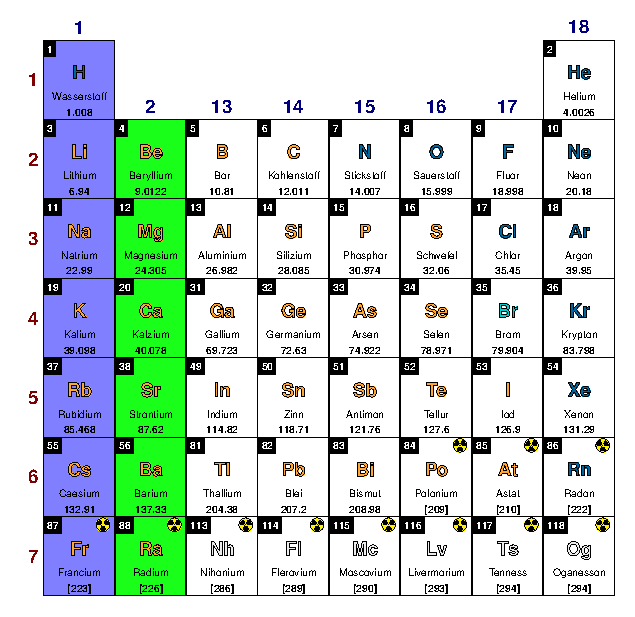
\includegraphics{manualfiles/pgfPT_user_compactPT.pdf}}
\end{center}
\tikz{\path[draw=green!70,rounded corners=2pt,fill=black!10!green!10,rounded corners=2pt] (0,0) rectangle ++(\textwidth,-4.5pt);}%
\endinput

\newpage%
\section{A few more examples}
\input{manualfiles/pgf-PeriodicTableManual_Examples.tex}%
\newpage\small%
\printindex%
\end{document}
